% Publication-ready elsarticle manuscript
% Status: Complete — full formal proofs, verified benchmarks, and literature audit.
\documentclass[preprint,12pt]{elsarticle}
\usepackage[margin=2.5cm]{geometry}
\usepackage[T1]{fontenc}
\usepackage{lmodern}
\usepackage{amsmath,amssymb,amsthm,mathtools}
\usepackage{mathrsfs}
\usepackage{graphicx}
\graphicspath{{../figures/}{figures/}{./}}
\usepackage{booktabs,array,tabularx}
\usepackage{tikz}
\usetikzlibrary{arrows.meta,positioning}
\usepackage{microtype}
\usepackage[hidelinks]{hyperref}
\biboptions{numbers,sort&compress}
\journal{Finite Fields and Their Applications}

\hypersetup{
  pdftitle={Joint Code-Dimension and k-Galois-Hull Enumerators for Repeated-Root Constacyclic Codes over Square-Free Affine Algebras},
  pdfauthor={Arun Kumar Yadav; Vipin Gupta; Pooja Soni; Manju Pruthi},
  pdfsubject={Coding theory}
}
\urlstyle{same}
\setlength{\emergencystretch}{1em}

\newcolumntype{L}[1]{>{\raggedright\arraybackslash}p{#1}}

\newcommand{\F}{\mathbb F}
\newcommand{\K}{\mathbb K}
\newcommand{\Z}{\mathbb Z}
\newcommand{\A}{\mathcal A}
\newcommand{\Fs}{\mathcal F_s}
\newcommand{\Os}{\mathcal O_s}
\newcommand{\Epoly}{\mathscr E}
\newcommand{\Hpoly}{\mathscr H}
\newcommand{\Hull}{\operatorname{Hull}}
\newcommand{\rank}{\operatorname{rank}}
\newcommand{\ord}{\operatorname{ord}}
\newcommand{\lcm}{\operatorname{lcm}}
\newcommand{\tr}{\operatorname{tr}}
\newcommand{\Var}{\operatorname{Var}}
\newcommand{\Cov}{\operatorname{Cov}}
\newcommand{\perpE}{\perp_E}
\newcommand{\Dk}{D_k}

\numberwithin{equation}{section}
\theoremstyle{plain}
\newtheorem{theorem}{Theorem}[section]
\newtheorem{lemma}[theorem]{Lemma}
\newtheorem{proposition}[theorem]{Proposition}
\newtheorem{corollary}[theorem]{Corollary}
\theoremstyle{definition}
\newtheorem{definition}[theorem]{Definition}
\newtheorem{example}[theorem]{Example}
\theoremstyle{remark}
\newtheorem{remark}[theorem]{Remark}

% Mark principal theorem statements visually.
\newenvironment{keyresult}
  {\par\addvspace{3pt}\noindent\rule{\linewidth}{0.4pt}\par\nobreak\addvspace{3pt}}
  {\par\nobreak\addvspace{3pt}\noindent\rule{\linewidth}{0.4pt}\par\addvspace{3pt}}

\begin{document}
\begin{frontmatter}
\title{Joint Code-Dimension and \texorpdfstring{$k$}{k}-Galois-Hull Enumerators for Repeated-Root Constacyclic Codes over Square-Free Affine Algebras}
\author[inst1]{Arun Kumar Yadav\corref{cor1}}
\ead{arunyadav0307@gmail.com}
\cortext[cor1]{Corresponding author}
\author[inst2]{Vipin Gupta}
\author[inst3]{Pooja Soni}
\author[inst4]{Manju Pruthi}

\affiliation[inst1]{organization={School of Basic and Applied Sciences, K.R. Mangalam University}, addressline={Sohna Road}, city={Gurugram}, postcode={122103}, state={Haryana}, country={India}}
\affiliation[inst2]{organization={Department of Mathematics, Gurugram University}, addressline={Sector 51}, city={Gurugram}, postcode={122003}, state={Haryana}, country={India}}
\affiliation[inst3]{organization={Department of Mathematics, Lovely Professional University}, addressline={Jalandhar-Delhi G.T. Road}, city={Phagwara}, postcode={144411}, state={Punjab}, country={India}}
\affiliation[inst4]{organization={Department of Mathematics, Indira Gandhi University}, addressline={Meerpur}, city={Rewari}, postcode={122502}, state={Haryana}, country={India}}

\begin{abstract}
Let $\A\cong\prod_{s=1}^{N}K_s$ be a finite commutative square-free affine
algebra over $\F_q$ ($q=p^e$, $K_s=\F_{q^{m_s}}$ with $m_s\ge 1$), let
$0\le k<e$, let $n=n'p^t\ge 1$ with $\gcd(n',p)=1$ and multiplicity $M=p^t$,
and let $\lambda=(\lambda_s)_{s=1}^{N}\in\A^*$ be any unit with unique $M$-th
roots $\lambda_{s,0}\in K_s^*$. We determine the exact bivariate generating
polynomial $\Epoly^{(M)}(U,Z)=\sum_C U^{\dim_{\F_q}C}Z^{\dim_{\F_q}\Hull_{\A,k}(C)}$
over all $(M+1)^{N_F}$ labeled $\A$-linear $\lambda$-constacyclic codes of
length $n$ without assuming $m_s=1$ or $\gcd(\ord(\lambda_s),n')=1$. Components
failing $\lambda_{s,0}^{\,1+p^{em_s-k}}=1$ have trivial $k$-Galois hulls for
every code, whereas on compatible components $\dim_{K_s}\Hull_k(C_s(e))$ splits
across inverse-Frobenius reciprocal orbits of $x^{n'}-\lambda_{s,0}$ as cyclic
sums of $\min\{e_i,M-e_{i+1}\}$. This yields a universal $(M+1)\times(M+1)$
transfer-matrix trace product for $\Epoly^{(M)}(U,Z)$ evaluating exponentially
large code spaces in polynomial time and recovering the simple-root theory at
$M=1$. From it we prove: (i) $p$-power invariance $2^{\sum_s|\Os|}$ of the
$k$-Galois LCD code count across all $t\ge 0$ for compatible twists; (ii) an
unconditional characterisation of the single-orbit support trapezoid
$\min\{R,M,aM-R\}\le H\le\min\{R,aM-R\}$ and the global Minkowski hull spectrum;
(iii) closed rational formulas for $\mathbb E[\eta_k]$, $\Var(\eta_k)$ across
the correlation regimes $a=1$, $a=2$, and $a\ge 3$, $\Cov(\kappa,\eta_k)=0$, and
conditional moments given $\kappa$; and (iv) exact enumerators for
self-orthogonal, dual-containing, and self-dual codes revealing a sharp
$p=2$ versus odd-$p$ dichotomy. All results are verified independently by
finite-field Gram-rank and raw quotient-polynomial computations across
characteristics $2$, $3$, and $5$.
\end{abstract}
\begin{keyword}
repeated-root constacyclic codes \sep $k$-Galois hulls \sep square-free affine algebras \sep exact enumeration \sep transfer matrices \sep LCD codes \sep self-dual codes
\MSC[2020] 94B05 \sep 94B15 \sep 05A15 \sep 11T71
\end{keyword}
\end{frontmatter}

\section{Introduction}\label{sec:intro}

The \emph{hull} $\Hull(C)=C\cap C^\perp$ of a linear code $C$ governs two
fundamental threads of modern coding theory: at one extreme, linear codes with
complementary duals ($\Hull(C)=\{0\}$, LCD codes) introduced by
Massey~\cite{massey1992,yangMassey1994} satisfy the Gilbert--Varshamov
bound~\cite{sendrier2004} and protect against side-channel and fault-injection
attacks~\cite{huffmanPless2003}; at the opposite and intermediate regimes, the
hull dimension directly determines the algorithmic complexity of
permutation-equivalence and automorphism-group algorithms~\cite{sendrier1997,bouyuklieva2026}
as well as the number of pre-shared maximally entangled ebits required to build
entanglement-assisted quantum error-correcting codes
(EAQECCs)~\cite{brun2006,wildeBrun2008,guendaJitmanGulliver2018,cao2021}.
Over a finite field of characteristic $p$, replacing the Euclidean inner product
by Fan and Zhang's $k$-Galois pairing~\cite{fanZhang2017} interpolates unifiedly
between Euclidean ($k=0$), Hermitian ($k=d/2$ for even degree $d$), and intermediate
Frobenius dualities~\cite{liuPan2020,fuLiu2022}.

For simple-root constacyclic codes ($\gcd(n,p)=1$), hull dimensions, average hull
dimensions, and enumerative counts over finite fields and ambient rings have been
investigated extensively~\cite{skersys2003,sangwisut2015,jitmanSangwisut2018,jitmanZ4,talbi2022,debnathConstacyclic2023,debnathCorrection2023,pathakZ4,gao2023,zhang2026,eldinSole2026,eldinLeroy2026,aliabadi2026}.
Recently, Debnath, Islam, Mart\'{\i}nez-Moro, and Prakash~\cite{debnathAffine2026}
studied $k$-Galois hulls of $\lambda$-constacyclic codes over square-free
commutative affine algebras $\A$ in the split case ($m_s=1$ on every simple
component), deriving a repeated-root hull-dimension formula under the cyclotomic
hypothesis $\gcd(\ord(\lambda),n')=1$ and $\ord(\lambda)\mid(1+p^{e-k})$
\cite[Theorem~8]{debnathAffine2026}, determining the cardinality of the hull-dimension
set in two special cases~\cite[Corollary~3.5]{debnathAffine2026}, and explicitly
posing in their Conclusion~\cite[p.~23]{debnathAffine2026} the open problem of
\emph{counting the number of constacyclic codes over $\A$ having each given
$k$-Galois hull dimension}. Related recent works examine first moments (average
Galois hull dimensions) over $\F_q$ and split rings $R_{m,q}=\F_q[u]/\langle
u^m-u\rangle$~\cite{debnathAverage2025} and existence criteria for hull dimensions
$1$ and $2$ over $\F_q$~\cite{debnathSmall2026}, while classical repeated-root
classifications treat restricted coprime parts $n'\in\{1,2,2\ell^m\}$ or Euclidean
LCD counts~\cite{castagnoli1991,vanLint1991,dinhLopezPermouth2004,dinh2010,dinh2012,chenDinhLiu2015,pangZhuLi2018}.

In the simple-root regime $\gcd(n,p)=1$ ($M=1$), each component quotient
$K_s[x]/\langle x^n-\lambda_s\rangle$ is semisimple, every constacyclic code
corresponds to a binary factor selection in $\{0,1\}^{\Fs}$, and the $k$-Galois
hull dimension reduces to a weighted count of circular $0\to 1$ boundaries in
$\{0,1\}^{a_O}$ governed by a $2\times 2$ transfer matrix (recovered here as the
$M=1$ specialisation in Corollary~\ref{cor:short-orbits}\textup{(c)}). When
$p\mid n$, writing $n=n'p^t$ with $\gcd(n',p)=1$ and $M=p^t\ge p$ changes the
algebraic and combinatorial picture qualitatively:
\begin{enumerate}
\item Ambient component rings $K_s[x]/\langle x^n-\lambda_s\rangle\cong
\prod_{f\in\Fs}K_s[x]/\langle f(x)^M\rangle$ are no longer semisimple products of
fields, but products of non-semisimple principal chain rings in which generator
exponents vary across the $(M+1)$-element alphabet $\{0,1,\dots,M\}$.
\item The base polynomial whose distinct irreducible factors $\Fs$ index ideals
is $x^{n'}-\lambda_{s,0}$ rather than $x^{n'}-\lambda_s$, where
$\lambda_{s,0}\in K_s^*$ is the unique $p^t$-th root of $\lambda_s$.
\item Simple-root circular run combinatorics on $\{0,1\}^{a_O}$ breaks down and
is replaced by cyclic sums of pairwise coupled edge minima
$\min\{e_i,M-e_{i+1}\}$, creating flat nonzero hull floors at height $w_O M$,
three distinct variance regimes ($a_O=1$, $a_O=2$, $a_O\ge 3$), and new self-dual
codes on odd-length orbits in characteristic $p=2$.
\end{enumerate}

\subsection*{Main contributions}

Figure~\ref{fig:workflow} summarises our end-to-end algebraic and enumerative
pipeline, and Table~\ref{tab:literature} contrasts our scope and results against
the closest existing literature. Specifically, for arbitrary $n=n'p^t$ ($t\ge 0$,
$M=p^t$), arbitrary non-split component degrees $m_s\ge 1$, arbitrary Galois
twists $0\le k<e$, and arbitrary units $\lambda\in\A^*$ (with zero coprimality
assumption between $\ord(\lambda_s)$ and $n'$):

\begin{figure}[htbp]
\centering
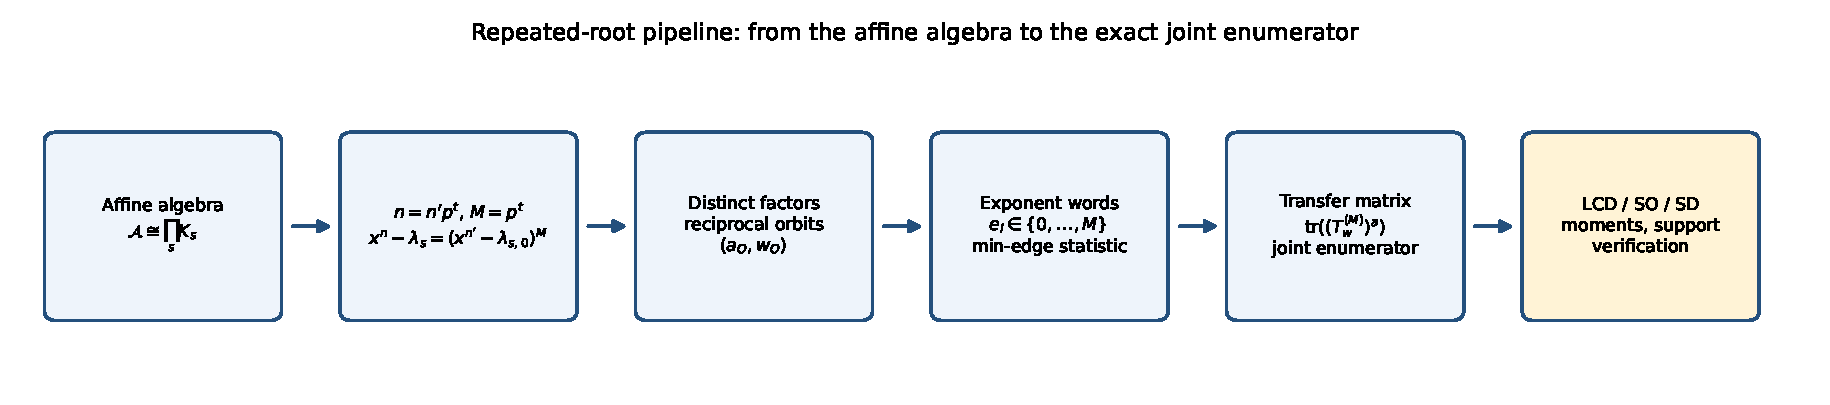
\includegraphics[width=0.96\textwidth]{fig1_workflow.pdf}
\caption{Overview of the exact repeated-root framework: CRT decomposition of the
square-free affine algebra $\A\cong\prod_{s=1}^{N}K_s$, pure-power reduction
$x^n-\lambda_s=(x^{n'}-\lambda_{s,0})^M$, partition into $\tau_{s,k}$-orbits
$(a_O,w_O)$, cyclic edge-minimum hull statistic on $\{0,\dots,M\}^{a_O}$,
$(M+1)\times(M+1)$ transfer-matrix trace product, and exact structural/statistical
consequences.}
\label{fig:workflow}
\end{figure}

\begin{enumerate}
\item \textbf{Repeated-root $k$-Galois duality and general twists
(Section~\ref{sec:duality}).} We prove directly, without any square-freeness or
order-coprimality hypothesis, that $\Dk(C_s(e))=\langle h_e^{\#_{s,k}}(x)\rangle$
(Theorem~\ref{thm:dual-generator}), prove that twist compatibility is invariant
under $p^t$-th roots ($\lambda_{s,0}^{\,1+p^{d_s-k}}=1\iff\lambda_s^{\,1+p^{d_s-k}}=1$,
Proposition~\ref{prop:compatibility}), completely resolve incompatible components
and mixed units $\lambda\in\A^*$ (Proposition~\ref{prop:incompatible}), and
establish full convention invariance of all dimension enumerators
(Remark~\ref{rem:conventions}).
\item \textbf{Single-code cyclic edge minimum and exact joint transfer-matrix
enumerator (Section~\ref{sec:enumerator}).} On every compatible component, we
express $\Hull_k(C_s(e))$ and $\dim_{K_s}\Hull_k(C_s(e))$ via cyclic sums of
$\min\{e_{O,i},M-e_{O,i+1}\}$ (Theorem~\ref{thm:hull-dimension}, reconciling and
strictly extending~\cite[Theorem~8]{debnathAffine2026}), and prove the universal
trace formula $\Epoly^{(M)}(U,Z)=\prod_{s,O}\tr(T_{w_O}^{(M)}(U,Z)^{a_O})\cdot
\prod_{s\in S_{\mathrm{inc}},f}\frac{1-U^{(M+1)m_s\deg f}}{1-U^{m_s\deg f}}$
(Theorem~\ref{thm:main}), answering the open enumeration problem of
\cite[p.~23]{debnathAffine2026} jointly with code dimension $\kappa(C)$ and
reducing at $M=1$ to an explicit circular-run binomial formula for the
simple-root regime (Corollary~\ref{cor:short-orbits}\textup{(c)}).
\item \textbf{LCD $p$-power invariance, exact support trapezoid, closed moments,
and extremal classes (Section~\ref{sec:consequences}).} We prove that $T_1^{(M)}(1,0)$
is a rank-$2$ matrix with unipotent Jordan block $\bigl(\begin{smallmatrix}1 & M\\
0 & 1\end{smallmatrix}\bigr)$, locking the compatible $k$-Galois LCD count at
$2^{\sum_s|\Os|}$ independently of $t=v_p(n)$ (Theorem~\ref{thm:lcd-invariance});
prove unconditionally that each single-orbit support is the exact lattice
trapezoid $\min\{R,M,aM-R\}\le H\le\min\{R,aM-R\}$ of cardinality
$aM+1+\lfloor(a-2)^2 M^2/4\rfloor$ ($a\ge 2$), yielding the global Minkowski hull
spectrum (Theorem~\ref{thm:support-trapezoid} and Corollary~\ref{cor:hull-spectrum});
derive exact rational formulas for $\mathbb E[\eta_k]$ (recovering the repeated-root
first moments of~\cite{debnathAverage2025} as a one-line special case; e.g.\ for
$q=2^6$, $n=28=7\cdot 4$, $k=3$, \eqref{eq:eta-mean} immediately gives
$\frac{4}{5}+6\cdot\frac{6}{5}=8$), $\Var(\eta_k)$ across all three regimes $a=1$
(even/odd $M$), $a=2$, and $a\ge 3$, $\Cov(\kappa,\eta_k)=0$, and conditional
moments $\mathbb E[\eta_k\mid\kappa]$, $\Var(\eta_k\mid\kappa)$
(Theorem~\ref{thm:moments} and Proposition~\ref{prop:conditional}); and give
exact enumerators for self-orthogonal, dual-containing, and self-dual codes
(Theorem~\ref{thm:extremal}).
\item \textbf{Polynomial-time algorithms and first-principles verification
(Section~\ref{sec:examples}).} Proposition~\ref{prop:algorithm} evaluates spaces
of size $5^{31}\approx 4.66\times 10^{21}$ in $<0.3\,\mathrm{s}$, while every
formula is verified independently by finite-field Gram-rank and raw
quotient-polynomial linear algebra across characteristics $2$, $3$, and $5$.
\end{enumerate}

\begin{table}[htbp]
\centering
\caption{Comparison of scope and results with closest existing works on hulls of constacyclic codes.}
\label{tab:literature}
\scriptsize
\setlength{\tabcolsep}{3.5pt}
\begin{tabular}{@{}L{2.8cm}L{1.7cm}L{1.3cm}L{1.5cm}L{2.3cm}L{2.1cm}L{2.5cm}@{}}
\toprule
Reference & Ambient ring & Length $n$ & Pairing & Twist $\lambda$ & Hull distribution & Moments, support \& extremal counts \\
\midrule
Sangwisut et al.~\cite{sangwisut2015} & $\F_q$ & $p\nmid n$ & Euclidean, Hermitian & $\lambda\in\{\pm 1\}$ & Marginal counts per $\eta$ & Mean only \\
Pang--Zhu--Li~\cite{pangZhuLi2018}; Chen et al.~\cite{chenDinhLiu2015} & $\F_q$ & $n'p^t$; $2\ell^m p^t$ & Euclidean ($k=0$) & $\lambda=1$ or restricted & LCD ($\eta=0$) only & LCD / SD counts \\
Debnath et al.~\cite{debnathConstacyclic2023,debnathCorrection2023} & $\F_q$ & $p\nmid n$ & $k$-Galois & Compatible $\lambda\in\F_q^*$ ($q$ restricted) & Marginal counts per $\eta$ & None \\
Debnath--Prakash~\cite{debnathAverage2025} & $\F_q$ and split $R_{m,q}$ & General $n$ & $k$-Galois & $\lambda\in\F_q^*$ / split & None & Unconditional mean $\mathbb E[\eta_k]$ only \\
Debnath et al.~\cite{debnathAffine2026} & Split $\A$ ($m_s=1$) & $n'p^t$ & $k$-Galois & $\gcd(\ord(\lambda),n')=1$, compatible & Open problem \cite[p.~23]{debnathAffine2026} & $|\operatorname{Spec}|$ in $2$ cases; LCD criterion \\
\textbf{Present work} & \textbf{General sq.-free $\A$ ($m_s\ge 1$)} & \textbf{All $n=n'p^t$ ($M=p^t\ge 1$)} & \textbf{$k$-Galois ($0\le k<e$)} & \textbf{Arbitrary $\lambda\in\A^*$ (comp.\ \& inc.)} & \textbf{Exact $(M+1)\!\times\!(M+1)$ trace product $\Epoly^{(M)}(U,Z)$} & \textbf{LCD invariance, support trapezoid, $\mathbb E$, $\Var$, cond.\ law, SO/DC/SD} \\
\bottomrule
\end{tabular}
\end{table}

\subsection*{Organisation of the paper}
Section~\ref{sec:setting} establishes the CRT structure, pure-power factorisation,
and global exponent-selection bijection. Section~\ref{sec:duality} proves the
repeated-root $k$-Galois dual generator, twist compatibility, incompatible-twist
collapse, and convention invariance. Section~\ref{sec:enumerator} proves the
single-code cyclic min-formula and the main transfer-matrix Theorem~\ref{thm:main}.
Section~\ref{sec:consequences} derives marginals, $p$-power LCD invariance, the
support trapezoid Theorem~\ref{thm:support-trapezoid}, exact moments, and extremal
code counts. Section~\ref{sec:examples} presents polynomial-time algorithms,
independent verification, and worked families, and Section~\ref{sec:conclusions}
records open directions.

\section{The repeated-root setting}\label{sec:setting}

This section fixes the algebraic framework used throughout the paper: the
square-free affine coefficient algebra and its fixed labeled finite-field
decomposition (\S\ref{sec:setup}), the pure-power factorisation of
repeated-root constacyclic moduli over each component field
(\S\ref{sec:factorisation}), the component and global exponent-selection
bijections generalising simple-root binary factor selections
(\S\ref{sec:selections}), and our standing assumptions and notation
(\S\ref{sec:assumptions}).

\subsection{Square-free affine algebras and CRT decomposition}\label{sec:setup}

Throughout the paper, $p$ is a prime and
\[
q=p^e,\qquad e\ge 1,
\]
is the order of the base field $\F_q$. Consider a multivariate commutative
affine $\F_q$-algebra presented as
\begin{equation}\label{eq:algebra}
\A=\F_q[X_1,\dots,X_\ell]\big/\langle t_1(X_1),\dots,t_\ell(X_\ell)\rangle,
\qquad \ell\ge 1,
\end{equation}
where each $t_i(X_i)\in\F_q[X_i]$ is monic, square-free over $\F_q$, and of
positive degree. This hypothesis makes $\A$ a reduced finite \'etale
$\F_q$-algebra and yields a canonical product decomposition once the component
labels are fixed.

\begin{proposition}[Square-free component decomposition]\label{prop:decomposition}
The affine algebra $\A$ in \eqref{eq:algebra} admits a fixed labeled $\F_q$-algebra
isomorphism
\begin{equation}\label{eq:decomp}
\A\cong\prod_{s=1}^{N} K_s,
\qquad
K_s=\F_{q^{m_s}}=\F_{p^{d_s}},
\qquad
d_s=e m_s,\quad m_s=[K_s:\F_q]\ge 1,
\end{equation}
together with pairwise orthogonal primitive idempotents $e_1,\dots,e_N\in\A$
satisfying $e_s e_{s'}=\delta_{s,s'}e_s$, $\sum_{s=1}^{N}e_s=1_\A$, and
$e_s\A\cong K_s$ for every $1\le s\le N$.
\end{proposition}

\begin{proof}
Because each $t_i$ is monic of positive degree and square-free over the perfect
field $\F_q$, each univariate quotient $\F_q[X_i]/\langle t_i(X_i)\rangle$
decomposes by the Chinese remainder theorem into a finite non-empty product of
finite extensions of $\F_q$ and is therefore finite \'etale over $\F_q$. The
presentation \eqref{eq:algebra} is the $\F_q$-tensor product of these factors,
so $\A$ is itself a non-zero finite \'etale $\F_q$-algebra and hence isomorphic
to a finite product of finite extensions $K_1,\dots,K_N$ of $\F_q$. Ordering the
factors fixes the isomorphism \eqref{eq:decomp} and identifies $e_s$ with the
tuple having $1_{K_s}$ in coordinate $s$ and $0$ elsewhere.
\end{proof}

We fix the labeled decomposition \eqref{eq:decomp} once and for all and write
elements of $\A$ in tuple coordinates as $a=(a_s)_{s=1}^{N}$ with $a_s\in K_s$.
Notice carefully the scope of the adjective \emph{square-free}: throughout this
paper, square-freeness is imposed solely on the defining polynomials
$t_1,\dots,t_\ell$ of the coefficient algebra $\A$ (so that $\A$ has no
nilpotent elements), whereas the constacyclic polynomial $x^n-\lambda_s$ in the
code length $n$ is allowed to have repeated roots whenever $p\mid n$.

\subsection{Repeated-root moduli and pure-power factorisation}\label{sec:factorisation}

Let $n\ge 1$ be an arbitrary integer and write
\begin{equation}\label{eq:length-decomp}
n=n'p^t,\qquad \gcd(n',p)=1,\qquad t=v_p(n)\ge 0,\qquad M:=p^t.
\end{equation}
The simple-root regime $\gcd(n,p)=1$ corresponds
to $t=0$ ($M=1$, $n=n'$) and is included uniformly in every statement below.

Fix a global shift unit $\lambda=(\lambda_s)_{s=1}^{N}\in\A^*=\prod_{s=1}^{N}K_s^*$.
For each component $1\le s\le N$, define the component constacyclic modulus
\begin{equation}\label{eq:modulus}
P_s(x):=x^n-\lambda_s\in K_s[x].
\end{equation}
Because the absolute Frobenius map $\operatorname{Frob}_s:a\mapsto a^p$ is a
field automorphism of $K_s=\F_{p^{d_s}}$, its $t$-fold iterate
$a\mapsto a^{p^t}=a^M$ is also an automorphism of $K_s$ (explicitly inverted by
$a\mapsto a^{p^{(-t)\bmod d_s}}$). Every component twist $\lambda_s\in K_s^*$
therefore admits a unique $M$-th root
\begin{equation}\label{eq:lambda0}
\lambda_{s,0}:=\operatorname{Frob}_s^{-t}(\lambda_s)\in K_s^*
\qquad\text{such that}\qquad
\lambda_{s,0}^M=\lambda_s.
\end{equation}

\begin{lemma}[Repeated-root factorisation]\label{lem:factorisation}
Let $n=n'p^t$ with $\gcd(n',p)=1$ and $M=p^t$, let $\lambda_s\in K_s^*$, and let
$\lambda_{s,0}\in K_s^*$ be defined by \eqref{eq:lambda0}. Denote by $\Fs$ the
set of distinct monic irreducible factors of the base polynomial
$P_{s,0}(x):=x^{n'}-\lambda_{s,0}$ in $K_s[x]$. Then $P_{s,0}(x)$ is square-free
over $K_s$, every $f\in\Fs$ satisfies $f(0)\neq 0$,
$\sum_{f\in\Fs}\deg f=n'$, and
\begin{equation}\label{eq:pure-power}
P_s(x)=x^n-\lambda_s=\bigl(x^{n'}-\lambda_{s,0}\bigr)^M
      =\prod_{f\in\Fs} f(x)^M.
\end{equation}
In particular, $\Fs$ is also the set of distinct monic irreducible factors of
$P_s(x)$ in $K_s[x]$, and each $f\in\Fs$ occurs in $P_s(x)$ with multiplicity
exactly $M$.
\end{lemma}

\begin{proof}
Existence and uniqueness of $\lambda_{s,0}\in K_s^*$ follow from bijectivity of
$a\mapsto a^{p^t}$ on the finite field $K_s$. Since $K_s[x]$ has characteristic
$p$, the map $g(x)\mapsto g(x)^p$ is a ring endomorphism of $K_s[x]$ sending $x$
to $x^p$ and each constant $c\in K_s$ to $c^p$; iterating it $t$ times gives
\[
\bigl(x^{n'}-\lambda_{s,0}\bigr)^M
 =\bigl(x^{n'}-\lambda_{s,0}\bigr)^{p^t}
 =x^{n'p^t}-\lambda_{s,0}^{p^t}
 =x^n-\lambda_s=P_s(x),
\]
as in the classical repeated-root reduction \cite{castagnoli1991,vanLint1991}.

Next, the formal derivative of $P_{s,0}(x)=x^{n'}-\lambda_{s,0}$ in $K_s[x]$ is
$P'_{s,0}(x)=n'x^{n'-1}$, with $n'\neq 0$ in $K_s$ because $\gcd(n',p)=1$. In an
algebraic closure $\overline{K}_s$, the only possible root of $x^{n'-1}$ is $0$,
whereas $P_{s,0}(0)=-\lambda_{s,0}\neq 0$. Thus $\gcd(P_{s,0},P'_{s,0})=1$, so
$P_{s,0}$ has no repeated roots in $\overline{K}_s$ and factors in the unique
factorisation domain $K_s[x]$ into pairwise distinct monic irreducibles
$P_{s,0}(x)=\prod_{f\in\Fs}f(x)$. Comparing degrees and constant terms gives
$\sum_{f\in\Fs}\deg f=\deg P_{s,0}=n'$ and
$\prod_{f\in\Fs}f(0)=-\lambda_{s,0}\neq 0$, whence $f(0)\neq 0$ for every
$f\in\Fs$. Raising $P_{s,0}(x)=\prod_{f\in\Fs}f(x)$ to the $M$-th power gives
\eqref{eq:pure-power}; unique factorisation in $K_s[x]$ identifies $\Fs$ with
the set of distinct monic irreducible factors of $P_s(x)$ and shows that each
occurs to exact power $M$.
\end{proof}

\begin{remark}\label{rem:no-ord-condition}
Lemma~\ref{lem:factorisation} is the entire factorisation input required in this
paper. Unlike explicit cyclotomic factorisation formulas over $\F_q$ such as
\cite[Section~2.4 and Theorem~8]{debnathAffine2026}, which impose $m_s=1$ and
$\gcd(\ord(\lambda),n')=1$, or explicit generator classifications for restricted
coprime parts $n'\in\{1,2,2\ell^m\}$ \cite{dinh2010,dinh2012,chenDinhLiu2015},
\eqref{eq:pure-power} holds for arbitrary $\lambda_s\in K_s^*$, arbitrary
extension degrees $m_s\ge 1$, and arbitrary coprime part $n'$. One bookkeeping
point is essential throughout: a code of length $n$ is an ideal modulo
$P_s(x)=x^n-\lambda_s$, whereas the distinct irreducible factors $\Fs$ are
determined by the base polynomial $x^{n'}-\lambda_{s,0}$, and in general
$\lambda_{s,0}\neq\lambda_s$ whenever $\lambda_s^{M-1}\neq 1$. Every concrete
example below therefore records both $\lambda_{s,0}$ and $\lambda_s=\lambda_{s,0}^M$.
\end{remark}

\subsection{Constacyclic codes and the exponent-selection bijection}\label{sec:selections}

Under the tuple identification $\A^n\cong\prod_{s=1}^{N}K_s^n$ induced by
\eqref{eq:decomp}, the ambient polynomial module for $\lambda$-constacyclic
codes is
\begin{equation}\label{eq:ambient}
\mathcal M_\lambda:=\A[x]/\langle x^n-\lambda\rangle
 \cong\prod_{s=1}^{N}K_s[x]/\langle P_s(x)\rangle
 \cong\prod_{s=1}^{N}K_s^n,
\end{equation}
where the second isomorphism sends a residue class $\sum_{i=0}^{n-1}c_ix^i$ to
its coefficient vector $(c_0,c_1,\dots,c_{n-1})$.

\begin{definition}\label{def:constacyclic-A}
For $\lambda\in\A^*$ and $n\ge 1$, the \emph{$\lambda$-constacyclic shift} on
$\A^n$ is the $\A$-linear map
\[
T_\lambda(c_0,c_1,\dots,c_{n-1}):=(\lambda c_{n-1},c_0,\dots,c_{n-2}).
\]
A \emph{$\lambda$-constacyclic code of length $n$ over $\A$} is an
$\A$-submodule $C\subseteq\A^n$ satisfying $T_\lambda(C)\subseteq C$. Under the
identification $\A^n\cong\mathcal M_\lambda$ in \eqref{eq:ambient}, $T_\lambda$
acts as multiplication by $x$, so the $\lambda$-constacyclic codes of length $n$
over $\A$ are precisely the ideals of $\mathcal M_\lambda$.
\end{definition}

\begin{remark}\label{rem:A-linear}
Neither Definition~\ref{def:constacyclic-A} nor \eqref{eq:ambient} requires
$\gcd(n,p)=1$. Throughout this paper, codes are required to be
$\A$-submodules of $\A^n$; $\F_q$-linear subspaces closed under $T_\lambda$ that
are not closed under scalar multiplication by $\A$ are outside the scope of our
enumeration.
\end{remark}

On each component $1\le s\le N$, an \emph{exponent selection} is a function
\[
e^{(s)}=(e_f)_{f\in\Fs}\in\{0,1,\dots,M\}^{\Fs};
\]
when the component index $s$ is clear from context we write $e=(e_f)_{f\in\Fs}$.
Associate to $e\in\{0,\dots,M\}^{\Fs}$ the monic generator polynomial, the monic
parity-check polynomial, and the component code
\begin{equation}\label{eq:gen-check}
g_e(x):=\prod_{f\in\Fs} f(x)^{e_f},\quad
h_e(x):=\frac{P_s(x)}{g_e(x)}=\prod_{f\in\Fs} f(x)^{M-e_f},\quad
C_s(e):=\langle g_e(x)\rangle\subseteq K_s[x]/\langle P_s(x)\rangle.
\end{equation}

\begin{lemma}[Component exponent-selection bijection]\label{lem:component-bijection}
For each $1\le s\le N$, the assignment $e\mapsto C_s(e)=\langle g_e(x)\rangle$
is a bijection from $\{0,\dots,M\}^{\Fs}$ onto the set of $\lambda_s$-constacyclic
codes of length $n$ over $K_s$. Moreover,
\begin{equation}\label{eq:comp-dim}
\dim_{K_s} C_s(e)=n-\sum_{f\in\Fs} e_f\deg f
                 =\sum_{f\in\Fs}(M-e_f)\deg f.
\end{equation}
\end{lemma}

\begin{proof}
Because $K_s[x]$ is a principal ideal domain, the lattice isomorphism theorem
puts the ideals of the quotient ring $K_s[x]/\langle P_s(x)\rangle$ in bijection
with the ideals of $K_s[x]$ containing $\langle P_s(x)\rangle$, and each such
ideal has a unique monic generator dividing $P_s(x)$. Indeed, if $g_1\mid P_s$
and $g_2\mid P_s$ are monic and generate the same ideal modulo $\langle P_s\rangle$,
then in $K_s[x]$ we have
\[
\langle g_1\rangle=\langle g_1,P_s\rangle=\langle g_2,P_s\rangle=\langle g_2\rangle,
\]
whence $g_1=g_2$ by monicity. By Lemma~\ref{lem:factorisation}, unique
factorisation in $K_s[x]$ puts the monic divisors of
$P_s(x)=\prod_{f\in\Fs}f(x)^M$ in bijection with tuples
$e=(e_f)_{f\in\Fs}\in\{0,\dots,M\}^{\Fs}$ via $e\mapsto g_e$.

Finally, $K_s[x]/\langle P_s\rangle\big/\langle g_e\rangle\cong K_s[x]/\langle g_e\rangle$
has $K_s$-dimension $\deg g_e=\sum_{f\in\Fs}e_f\deg f$, so
$\dim_{K_s}C_s(e)=n-\deg g_e$. Since $n=Mn'=M\sum_{f\in\Fs}\deg f$ by
Lemma~\ref{lem:factorisation}, subtracting $\sum_{f\in\Fs}e_f\deg f$ yields the
second expression in \eqref{eq:comp-dim}.
\end{proof}

Define the global exponent-selection space, total distinct-factor count, and
ambient $\F_q$-dimension by
\begin{equation}\label{eq:selection-space}
\mathscr C^{(M)}:=\prod_{s=1}^{N}\{0,1,\dots,M\}^{\Fs},
\qquad
N_F:=\sum_{s=1}^{N}|\Fs|,
\qquad
W:=n\sum_{s=1}^{N}m_s.
\end{equation}
For $e=(e^{(s)})_{s=1}^{N}\in\mathscr C^{(M)}$, define the global product code
\begin{equation}\label{eq:global-code}
C(e):=\prod_{s=1}^{N} C_s\bigl(e^{(s)}\bigr)
     \subseteq\prod_{s=1}^{N}K_s^n\cong\A^n,
\end{equation}
generated in $\mathcal M_\lambda$ by the tuple element $g_e:=(g_{e^{(s)}})_{s=1}^{N}$.

\begin{lemma}[Global exponent-selection bijection]\label{lem:global-bijection}
Every $\lambda$-constacyclic code $C\subseteq\A^n$ decomposes uniquely as
$C=\bigoplus_{s=1}^{N}e_s C$, where each $e_s C$ is an ideal of
$e_s\mathcal M_\lambda\cong K_s[x]/\langle P_s(x)\rangle$. Consequently, the map
\[
\mathscr C^{(M)}\longrightarrow
\{\lambda\text{-constacyclic codes of length }n\text{ over }\A\},
\qquad
e\longmapsto C(e),
\]
is a bijection. In particular, the total number of labeled $\lambda$-constacyclic
codes of length $n$ over $\A$ is
\begin{equation}\label{eq:total-codes-setting}
\bigl|\mathscr C^{(M)}\bigr|=(M+1)^{N_F},
\end{equation}
and the global $\F_q$-dimension of $C(e)$ is
\begin{equation}\label{eq:global-dim}
\kappa\bigl(C(e)\bigr):=\dim_{\F_q}C(e)
 =\sum_{s=1}^{N}m_s\dim_{K_s}C_s\bigl(e^{(s)}\bigr)
 =\sum_{s=1}^{N}\sum_{f\in\Fs} m_s(\deg f)\,(M-e_f).
\end{equation}
\end{lemma}

\begin{proof}
Let $e_1,\dots,e_N\in\A$ be the orthogonal primitive idempotents of
Proposition~\ref{prop:decomposition}. For any ideal $C\subseteq\mathcal M_\lambda$,
$\A$-linearity gives $e_s C\subseteq C$, and $\sum_{s=1}^{N}e_s=1_\A$ with
$e_s e_{s'}=\delta_{s,s'}e_s$ gives the internal direct sum
$C=\bigoplus_{s=1}^{N}e_s C$. Multiplication by $e_s$ projects $\mathcal M_\lambda$
surjectively onto
\[
e_s\mathcal M_\lambda
 =e_s\A[x]\big/\langle e_s(x^n-\lambda)\rangle
 \cong K_s[x]/\langle P_s(x)\rangle,
\]
carrying the $\A[x]$-submodule $C$ to a $K_s[x]$-ideal $e_s C$; none of these
idempotent steps uses square-freeness of $P_s(x)$
(where each component ring
$K_s[x]/\langle P_s(x)\rangle\cong\prod_{f\in\Fs}K_s[x]/\langle f(x)^M\rangle$
is a product of local principal chain rings rather than fields whenever $M>1$).

Applying Lemma~\ref{lem:component-bijection} to each component ideal $e_s C$
produces a unique $e^{(s)}\in\{0,\dots,M\}^{\Fs}$ with $e_s C=C_s(e^{(s)})$,
proving surjectivity. Conversely, each $C(e)$ in \eqref{eq:global-code} is an
ideal of $\prod_{s=1}^{N}K_s[x]/\langle P_s(x)\rangle\cong\mathcal M_\lambda$,
and if $C(e)=C(e')$ then multiplying by $e_s$ yields
$C_s(e^{(s)})=C_s(e'^{(s)})$ and hence $e^{(s)}=e'^{(s)}$ for all $s$ by
Lemma~\ref{lem:component-bijection}. Thus $e\mapsto C(e)$ is bijective, so
$|\mathscr C^{(M)}|=\prod_{s=1}^{N}(M+1)^{|\Fs|}=(M+1)^{N_F}$. Since
$[K_s:\F_q]=m_s$, summing the $\F_q$-dimensions of the direct summands and
substituting \eqref{eq:comp-dim} gives \eqref{eq:global-dim}.
\end{proof}

\subsection{Standing assumptions and notation}\label{sec:assumptions}

For ease of reference, we collect our standing conventions in one place:
\begin{enumerate}
\item[\textbf{A1.}] $\A$ is square-free over $\F_q$ ($q=p^e$, $e\ge 1$) with fixed
labeled decomposition $\A\cong\prod_{s=1}^{N}K_s$, $K_s=\F_{q^{m_s}}=\F_{p^{d_s}}$,
$d_s=em_s$; only the constacyclic modulus $P_s(x)=x^n-\lambda_s$ may have
repeated roots.
\item[\textbf{A2.}] $n=n'p^t\ge 1$ with $\gcd(n',p)=1$, $t=v_p(n)\ge 0$, and
multiplicity $M=p^t$ ($t=0$, i.e.\ $M=1$, is the simple-root case).
\item[\textbf{A3.}] $\lambda=(\lambda_s)_{s=1}^{N}\in\A^*$ is an arbitrary unit,
with unique component $M$-th roots $\lambda_{s,0}\in K_s^*$ satisfying
$\lambda_{s,0}^M=\lambda_s$. The reciprocal-orbit product is formulated for
compatible components (\S\ref{sec:compatibility}), while incompatible components
are resolved completely by Proposition~\ref{prop:incompatible}.
\item[\textbf{A4.}] Codes are $\A$-linear $\lambda$-constacyclic codes of length
$n$ in the sense of Definition~\ref{def:constacyclic-A}.
\item[\textbf{A5.}] Global dimensions ($\kappa$, $\eta_k$, $W$) are taken over
$\F_q$; component dimensions over $K_s$ multiply by $m_s=[K_s:\F_q]$.
\item[\textbf{A6.}] Counting is labeled: distinct exponent selections
$e\neq e'$ in $\mathscr C^{(M)}$ count as distinct codes in $\A^n$, without
quotienting by monomial, Galois, or ring automorphisms.
\item[\textbf{A7.}] The $k$-Galois pairing ($0\le k<e$) is code-first,
$\langle x,y\rangle_{s,k}=\sum_{i=0}^{n-1}x_i y_i^{p^k}$
(see Remark~\ref{rem:conventions} for the candidate-first convention).
\item[\textbf{A8.}] Probabilistic expectations, variances, and conditional laws
refer to the uniform measure $\mathbb P(C(e))=(M+1)^{-N_F}$ on $\mathscr C^{(M)}$.
\end{enumerate}

The symbols used throughout the manuscript are summarised in
Table~\ref{tab:nomenclature}; none is overloaded elsewhere in the text.

\begin{table}[htbp]
\centering
\caption{Master notation and dimension conventions used throughout the paper.}
\label{tab:nomenclature}
\small
\begin{tabularx}{\textwidth}{@{}lX@{}}
\toprule
Symbol & Meaning \\
\midrule
$p$, $q=p^e$, $k$ & prime characteristic, base-field order ($e\ge 1$), and Galois twist exponent ($0\le k<e$) \\
$s\in\{1,\dots,N\}$ & fixed component index in $\A\cong\prod_{s=1}^{N}K_s$ \\
$K_s=\F_{q^{m_s}}=\F_{p^{d_s}}$ & $s$-th component field, with $m_s=[K_s:\F_q]$ and $d_s=em_s$ \\
$n=n'p^t$, $M=p^t$ & code length with $\gcd(n',p)=1$, $t=v_p(n)\ge 0$, and factor multiplicity $M$ \\
$\lambda_s$, $\lambda_{s,0}\in K_s^*$ & component twist and its unique $M$-th root satisfying $\lambda_{s,0}^M=\lambda_s$ \\
$P_s(x)=x^n-\lambda_s$ & component constacyclic modulus, equal to $(x^{n'}-\lambda_{s,0})^M$ \\
$\Fs$ & set of distinct monic irreducible factors of $x^{n'}-\lambda_{s,0}$ over $K_s$ \\
$e=(e_f)_{f\in\Fs}$, $\mathscr C^{(M)}$ & exponent selection with $0\le e_f\le M$, and global selection space $\prod_s\{0,\dots,M\}^{\Fs}$ \\
$g_e(x)$, $h_e(x)$ & generator $\prod_{f\in\Fs}f^{e_f}$ and parity-check polynomial $P_s/g_e=\prod_{f\in\Fs}f^{M-e_f}$ \\
$C_s(e)$, $C(e)$ & component code $\langle g_e\rangle\subseteq K_s[x]/\langle P_s\rangle$ and global code $\prod_s C_s(e^{(s)})\subseteq\A^n$ \\
$\sigma_{s,k}$, $\rho_{s,k}$ & $k$-Frobenius $a\mapsto a^{p^k}$ on $K_s$ and its inverse $a\mapsto a^{p^{d_s-k}}$ \\
$f^{\#_{s,k}}$, $\tau_{s,k}$ & normalised inverse-Frobenius reciprocal \eqref{eq:reciprocal} and induced permutation of $\Fs$ \\
$\Os$, $O$, $a_O$, $d_O$, $w_O$ & orbit set of $\tau_{s,k}$, an orbit $O\in\Os$, length $|O|$, factor degree, and $\F_q$-weight $m_s d_O$ \\
$e_{O,i}$ ($i\in\Z/a_O\Z$) & cyclic exponent word along $O$, ordered by $\tau_{s,k}(f_{O,i})=f_{O,i+1}$ \\
$D_k(\cdot)$, $\Hull_k(\cdot)$ & component $k$-Galois dual and hull; globally $D_{\A,k}(\cdot)$ and $\Hull_{\A,k}(\cdot)$ \\
$\kappa(C)$, $\eta_k(C)$ & $\F_q$-dimensions $\dim_{\F_q}C$ and $\dim_{\F_q}\Hull_{\A,k}(C)$ \\
$N_F$, $W$ & total distinct-factor count $\sum_s|\Fs|$ and ambient $\F_q$-dimension $n\sum_s m_s$ \\
$U$, $Z$ & formal variables marking $\kappa(C)$ and $\eta_k(C)$ in generating polynomials \\
$\Epoly^{(M)}(U,Z)$, $\Hpoly^{(M)}(Z)$ & exact joint enumerator and marginal hull polynomial $\Epoly^{(M)}(1,Z)$ \\
$T^{(M)}_w(U,Z)$ & $(M+1)\times(M+1)$ transfer matrix on state set $\{0,\dots,M\}$ \\
$\Phi_j(\kappa)$ & factorial-moment coefficient $[U^\kappa]\,\partial_Z^j\Epoly^{(M)}(U,Z)\big|_{Z=1}$ ($j=0,1,2$) \\
\bottomrule
\end{tabularx}
\end{table}

\section{\texorpdfstring{$k$}{k}-Galois duality}\label{sec:duality}

We next determine the $k$-Galois dual of an arbitrary repeated-root constacyclic
code over $\A$ and classify twist compatibility across all units $\lambda\in\A^*$.
We recall the componentwise and global $k$-Galois pairings (\S\ref{sec:pairing})
and the normalised inverse-Frobenius reciprocal (\S\ref{sec:reciprocal}), recheck
the Euclidean dual of a constacyclic ideal directly without any square-freeness
assumption and deduce the repeated-root $k$-Galois dual generator
(\S\ref{sec:duals}), and establish the unchanged compatibility criterion together
with the exact behaviour of incompatible twists and dual conventions
(\S\ref{sec:compatibility}).

\subsection{Component and global \texorpdfstring{$k$}{k}-Galois pairings}\label{sec:pairing}

Fix an integer $k$ with $0\le k<e$. On each component field
$K_s=\F_{q^{m_s}}=\F_{p^{d_s}}$ ($d_s=em_s>k$), define the field automorphisms
\begin{equation}\label{eq:frobenius}
\sigma_{s,k}(a):=a^{p^k},
\qquad
\rho_{s,k}(a):=\sigma_{s,k}^{-1}(a)=a^{p^{d_s-k}}
\qquad(a\in K_s).
\end{equation}
For vectors $x=(x_0,\dots,x_{n-1})$ and $y=(y_0,\dots,y_{n-1})$ in $K_s^n$, the
code-first $k$-Galois pairing \cite{fanZhang2017} is
\begin{equation}\label{eq:pairing}
\langle x,y\rangle_{s,k}:=\sum_{i=0}^{n-1}x_i\sigma_{s,k}(y_i)
 =\sum_{i=0}^{n-1}x_i y_i^{p^k},
\end{equation}
and the component $k$-Galois dual and $k$-Galois hull of a $K_s$-linear code
$C\subseteq K_s^n$ are
\[
\Dk(C):=\{y\in K_s^n:\langle c,y\rangle_{s,k}=0\text{ for all }c\in C\},
\qquad
\Hull_k(C):=C\cap\Dk(C).
\]
When $k=0$, \eqref{eq:pairing} is the standard Euclidean inner product on every
component $K_s^n$; we write $C^{\perpE}:=D_0(C)$ for the Euclidean dual. On
$K_s=\F_{p^{d_s}}$, the pairing \eqref{eq:pairing} is Hermitian if and only if
$d_s$ is even and $k=d_s/2$; in particular, when $e$ is even, the choice $k=e/2$
is Hermitian on components with $m_s=1$ and never Hermitian on components with
$m_s>1$.

Globally on $\A\cong\prod_{s=1}^{N}K_s$, set
$\sigma_{\A,k}((a_s)_s):=(\sigma_{s,k}(a_s))_s$ and
$\rho_{\A,k}((a_s)_s):=(\rho_{s,k}(a_s))_s$, and define the $\A$-valued pairing
on $\A^n$ by
\begin{equation}\label{eq:global-pairing}
\langle x,y\rangle_{\A,k}:=\sum_{i=0}^{n-1}x_i\sigma_{\A,k}(y_i)
 =\bigl(\langle x_s,y_s\rangle_{s,k}\bigr)_{s=1}^{N},
\end{equation}
with global dual and hull
\[
D_{\A,k}(C):=\{y\in\A^n:\langle c,y\rangle_{\A,k}=0_\A\text{ for all }c\in C\},
\qquad
\Hull_{\A,k}(C):=C\cap D_{\A,k}(C).
\]

\begin{lemma}[Dual translation and product decomposition]\label{lem:global-duality}
Let $n\ge 1$ be arbitrary.
\begin{enumerate}
\item[\textup{(a)}] For every $K_s$-linear subspace $C\subseteq K_s^n$, applying
$\rho_{s,k}$ coordinatewise gives
\begin{equation}\label{eq:dual-translation}
\Dk(C)=\rho_{s,k}\bigl(C^{\perpE}\bigr),
\qquad\text{so}\qquad
\dim_{K_s}\Dk(C)=n-\dim_{K_s}C.
\end{equation}
\item[\textup{(b)}] For every global exponent selection
$e=(e^{(s)})_{s=1}^{N}\in\mathscr C^{(M)}$,
\begin{equation}\label{eq:global-dual-hull}
D_{\A,k}\bigl(C(e)\bigr)=\prod_{s=1}^{N}\Dk\bigl(C_s(e^{(s)})\bigr),
\qquad
\Hull_{\A,k}\bigl(C(e)\bigr)=\prod_{s=1}^{N}\Hull_k\bigl(C_s(e^{(s)})\bigr),
\end{equation}
and the global $\F_q$-hull dimension is
\begin{equation}\label{eq:global-hull-dim}
\eta_k\bigl(C(e)\bigr):=\dim_{\F_q}\Hull_{\A,k}\bigl(C(e)\bigr)
 =\sum_{s=1}^{N} m_s\dim_{K_s}\Hull_k\bigl(C_s(e^{(s)})\bigr).
\end{equation}
\end{enumerate}
\end{lemma}

\begin{proof}
For \textup{(a)}, a vector $y\in K_s^n$ satisfies
$\sum_{i=0}^{n-1}c_i\sigma_{s,k}(y_i)=0$ for all $c\in C$ if and only if
$z:=\sigma_{s,k}(y)\in C^{\perpE}$, i.e.\ $y=\rho_{s,k}(z)$ with
$z\in C^{\perpE}$. Since $\rho_{s,k}:K_s^n\to K_s^n$ is a bijection of finite
sets and a $\rho_{s,k}$-semilinear vector-space isomorphism,
$\dim_{K_s}\Dk(C)=\dim_{K_s}C^{\perpE}=n-\dim_{K_s}C$.

For \textup{(b)}, testing $\langle c,y\rangle_{\A,k}=0_\A$ in
\eqref{eq:global-pairing} against vectors $c\in C(e)$ supported solely in
coordinate $s$ shows $y_s\in\Dk(C_s(e^{(s)}))$ for each $s$, and the converse
inclusion is immediate componentwise. Intersecting with
$C(e)=\prod_{s=1}^{N}C_s(e^{(s)})$ gives the hull decomposition in
\eqref{eq:global-dual-hull}, and summing $\F_q$-dimensions with $[K_s:\F_q]=m_s$
gives \eqref{eq:global-hull-dim}. None of these vector-space arguments depends
on $\gcd(n,p)$.
\end{proof}

\subsection{The inverse-Frobenius reciprocal}\label{sec:reciprocal}

For a monic polynomial $f(x)=\sum_{i=0}^{r}f_i x^i\in K_s[x]$ of degree $r\ge 0$
with $f_0\neq 0$, define its normalised inverse-Frobenius reciprocal by
\begin{equation}\label{eq:reciprocal}
f^{\#_{s,k}}(x):=\rho_{s,k}(f_0)^{-1}\sum_{i=0}^{r}\rho_{s,k}(f_i)\,x^{r-i}.
\end{equation}

\begin{lemma}[Properties of the twisted reciprocal]\label{lem:reciprocal-props}
Let $f,g\in K_s[x]$ be monic polynomials with nonzero constant terms.
\begin{enumerate}
\item[\textup{(a)}] $f^{\#_{s,k}}$ is monic of degree $\deg f$ with constant term
$\rho_{s,k}(f_0)^{-1}\neq 0$, and the map $f\mapsto f^{\#_{s,k}}$ is a bijection
on the set of monic polynomials in $K_s[x]$ with nonzero constant term, inverted
by $h(x)\mapsto \sigma_{s,k}(h_0)^{-1}\sum_{i=0}^{\deg h}\sigma_{s,k}(h_i)x^{\deg h-i}$.
\item[\textup{(b)}] $(fg)^{\#_{s,k}}=f^{\#_{s,k}}g^{\#_{s,k}}$; in particular,
\begin{equation}\label{eq:reciprocal-power}
(f^m)^{\#_{s,k}}=\bigl(f^{\#_{s,k}}\bigr)^m
\qquad\text{for every integer }m\ge 0.
\end{equation}
\item[\textup{(c)}] $f^{\#_{s,k}}$ is irreducible in $K_s[x]$ if and only if $f$
is irreducible in $K_s[x]$. Moreover, if $L/K_s$ is a finite extension and
$\alpha\in L^*$ satisfies $f(\alpha)=0$, then
$f^{\#_{s,k}}\bigl(\alpha^{-p^{d_s-k}}\bigr)=0$.
\end{enumerate}
\end{lemma}

\begin{proof}
In \eqref{eq:reciprocal} the coefficient of $x^r$ is
$\rho_{s,k}(f_0)^{-1}\rho_{s,k}(f_0)=1$ and the constant term is
$\rho_{s,k}(f_0)^{-1}\rho_{s,k}(1)=\rho_{s,k}(f_0)^{-1}\neq 0$; applying the
displayed $\sigma_{s,k}$-reciprocal directly returns $f$, proving \textup{(a)}.
Writing \eqref{eq:reciprocal} in $K_s[x,x^{-1}]$ as
\begin{equation}\label{eq:reciprocal-laurent}
f^{\#_{s,k}}(x)=\rho_{s,k}(f_0)^{-1}x^{\deg f}\,(\widetilde{\rho}_{s,k}f)(x^{-1}),
\end{equation}
where $\widetilde{\rho}_{s,k}:K_s[x]\to K_s[x]$ applies $\rho_{s,k}$
coefficientwise, yields $(fg)^{\#_{s,k}}=f^{\#_{s,k}}g^{\#_{s,k}}$ and hence
\eqref{eq:reciprocal-power} by induction on $m$ (with $1^{\#_{s,k}}=1$ at $m=0$).
By \textup{(a)} and \textup{(b)}, non-trivial monic factorisations of $f$ correspond
bijectively to non-trivial monic factorisations of $f^{\#_{s,k}}$, so
irreducibility is preserved. Finally, extend $\alpha\mapsto\alpha^{p^{d_s-k}}$ to
$L$; if $f(\alpha)=0$, evaluating \eqref{eq:reciprocal-laurent} at
$\beta=\alpha^{-p^{d_s-k}}\in L^*$ gives
\[
\bigl(\widetilde{\rho}_{s,k}f\bigr)(\beta^{-1})
 =\sum_{i=0}^{r}f_i^{p^{d_s-k}}\bigl(\alpha^{p^{d_s-k}}\bigr)^i
 =\bigl(f(\alpha)\bigr)^{p^{d_s-k}}=0,
\]
whence $f^{\#_{s,k}}(\beta)=0$, establishing \textup{(c)}.
\end{proof}

\subsection{Euclidean and \texorpdfstring{$k$}{k}-Galois dual generators}\label{sec:duals}

The bridge from Euclidean duality to $k$-Galois duality in
Lemma~\ref{lem:global-duality}\textup{(a)} requires the generator polynomial of
the Euclidean dual of a constacyclic code of arbitrary length $n$. We verify this
directly line by line so it is transparent that repeated roots cause no
obstruction.

\begin{lemma}[Euclidean dual without square-freeness]\label{lem:euclidean-dual}
Let $K$ be a finite field, $a\in K^*$, and $n\ge 1$ be arbitrary. Let
$G(x)\in K[x]$ be a monic divisor of $x^n-a$, set $H(x):=(x^n-a)/G(x)$, and write
\[
H^*(x):=H(0)^{-1}\sum_{v=0}^{\deg H} H_v x^{\deg H-v}
\]
for the normalised ordinary reciprocal of $H(x)=\sum_{v=0}^{\deg H}H_v x^v$.
Under the coefficient-vector identification $K[x]/\langle x^n-a\rangle\cong K^n$,
the Euclidean dual $\langle G(x)\rangle^{\perpE}$ is the $a^{-1}$-constacyclic
ideal generated by $H^*(x)$ in $K[x]/\langle x^n-a^{-1}\rangle$.
\end{lemma}

\begin{proof}
Put $r:=\deg G$ and $h:=\deg H$, so $0\le r,h\le n$, $r+h=n$, and both $G$ and
$H$ are monic with $G(0)H(0)=(GH)(0)=-a\neq 0$. Thus $G^*(x)=G(0)^{-1}x^r G(x^{-1})$
and $H^*(x)=H(0)^{-1}x^h H(x^{-1})$ are well-defined monic polynomials of degrees
$r$ and $h$ in $K[x]$, and in $K[x,x^{-1}]$ (hence in $K[x]$) we have
\begin{equation}\label{eq:reciprocal-product}
G^*(x)\,H^*(x)
 =\bigl(G(0)H(0)\bigr)^{-1}x^{r+h}G(x^{-1})H(x^{-1})
 =(-a)^{-1}x^n(x^{-n}-a)
 =x^n-a^{-1}.
\end{equation}
In particular, $H^*(x)$ is a monic divisor of $x^n-a^{-1}$, so
$\langle H^*(x)\rangle$ is an ideal of $K[x]/\langle x^n-a^{-1}\rangle$ of
$K$-dimension $n-h=r$ spanned by the non-wrapped shifts $\{x^j H^*(x):0\le j<r\}$,
while $\langle G(x)\rangle\subseteq K[x]/\langle x^n-a\rangle$ has $K$-dimension
$n-r=h$ spanned by $\{x^i G(x):0\le i<h\}$ (an empty spanning set having span
$\{0\}$ when $r=0$ or $h=0$).

Write $G(x)=\sum_{u=0}^{r}G_u x^u$. For any $0\le i<h$ and $0\le j<r$, every
term in $x^i G(x)$ and $x^j H^*(x)$ has degree strictly less than $n$, so the
Euclidean inner product of their coefficient vectors in $K^n$ is
\begin{align*}
\langle x^i G,\,x^j H^*\rangle_{s,0}
 &=H(0)^{-1}\sum_{\substack{0\le u\le r,\;0\le v\le h\\ i+u=j+h-v}} G_u H_v \\
 &=H(0)^{-1}[x^{h-i+j}]\bigl(G(x)H(x)\bigr)
  =H(0)^{-1}[x^{h-i+j}](x^n-a)=0,
\end{align*}
because $0\le i\le h-1$ and $0\le j\le r-1$ imply $1\le h-i+j\le h+r-1=n-1$.
Hence $\langle H^*(x)\rangle\subseteq\langle G(x)\rangle^{\perpE}$, and equality
follows from $\dim_K\langle H^*(x)\rangle=r=n-h=\dim_K\langle G(x)\rangle^{\perpE}$.
No step uses that $x^n-a$ is square-free; multiplicities are carried along by $H$.
\end{proof}

\begin{theorem}[\texorpdfstring{$k$}{k}-Galois dual generator]\label{thm:dual-generator}
Let $e\in\{0,\dots,M\}^{\Fs}$, let $C_s(e)=\langle g_e(x)\rangle\subseteq K_s[x]/\langle P_s(x)\rangle$,
and let $h_e(x)=P_s(x)/g_e(x)=\prod_{f\in\Fs}f(x)^{M-e_f}$ be as in
\eqref{eq:gen-check}. Then the $k$-Galois dual $\Dk(C_s(e))$ is the
$\lambda_s^{-p^{d_s-k}}$-constacyclic ideal in
$K_s[x]/\langle x^n-\lambda_s^{-p^{d_s-k}}\rangle$ generated by the monic
polynomial
\begin{equation}\label{eq:dual-gen-general}
h_e^{\#_{s,k}}(x)=\prod_{f\in\Fs}\bigl(f^{\#_{s,k}}(x)\bigr)^{M-e_f}.
\end{equation}
If, in addition, $f\mapsto f^{\#_{s,k}}$ restricts to a bijection
$\tau_{s,k}:\Fs\to\Fs$, then
\begin{equation}\label{eq:dual-gen-compatible}
h_e^{\#_{s,k}}(x)=\prod_{f\in\Fs} f(x)^{\,M-e_{\tau_{s,k}^{-1}(f)}},
\end{equation}
so the multiplicity of $f\in\Fs$ in the dual generator is $M-e_{\tau_{s,k}^{-1}(f)}$.
\end{theorem}

\begin{proof}
By Lemma~\ref{lem:euclidean-dual} with $K=K_s$, $a=\lambda_s$, $G=g_e$, and
$H=h_e$, the Euclidean dual $C_s(e)^{\perpE}$ is the $\lambda_s^{-1}$-constacyclic
ideal $\langle h_e^*(x)\rangle\subseteq K_s[x]/\langle x^n-\lambda_s^{-1}\rangle$.
Coefficientwise application of $\rho_{s,k}$ defines a ring automorphism
$\widetilde{\rho}_{s,k}:K_s[x]\to K_s[x]$ that sends $x^n-\lambda_s^{-1}$ to
$x^n-\rho_{s,k}(\lambda_s^{-1})=x^n-\lambda_s^{-p^{d_s-k}}$ and sends $h_e^*(x)$
to
\[
\widetilde{\rho}_{s,k}\bigl(h_e^*(x)\bigr)
 =\rho_{s,k}\bigl(h_e(0)\bigr)^{-1}
   \sum_{v=0}^{\deg h_e}\rho_{s,k}(h_{e,v})x^{\deg h_e-v}
 =h_e^{\#_{s,k}}(x).
\]
Under the coefficient-vector identification $K_s[x]/\langle x^n-\mu\rangle\cong K_s^n$,
$\widetilde{\rho}_{s,k}$ acts on $K_s^n$ coordinatewise as $\rho_{s,k}$.
Combining this with $\Dk(C_s(e))=\rho_{s,k}(C_s(e)^{\perpE})$ from
Lemma~\ref{lem:global-duality}\textup{(a)} shows that $\Dk(C_s(e))$ is the
$\lambda_s^{-p^{d_s-k}}$-constacyclic ideal generated by $h_e^{\#_{s,k}}(x)$.

Applying Lemma~\ref{lem:reciprocal-props}\textup{(b)} to
$h_e=\prod_{f\in\Fs}f^{M-e_f}$ gives \eqref{eq:dual-gen-general}. When
$\tau_{s,k}(f)=f^{\#_{s,k}}$ permutes $\Fs$, reindexing the product in
\eqref{eq:dual-gen-general} via $f'=\tau_{s,k}(f)$ (so $f=\tau_{s,k}^{-1}(f')$)
yields \eqref{eq:dual-gen-compatible}.
\end{proof}

\subsection{Compatibility, general twists, and dual conventions}\label{sec:compatibility}

We now show that passing from the length-$n$ twist $\lambda_s$ to its unique
$M$-th root $\lambda_{s,0}$ leaves the simple-root twist-compatibility criterion
completely unchanged.

\begin{proposition}[Compatibility in the repeated-root setting]\label{prop:compatibility}
For each component $1\le s\le N$, the following conditions are equivalent:
\begin{enumerate}
\item[\textup{(a)}] $\lambda_{s,0}^{\,1+p^{d_s-k}}=1$;
\item[\textup{(b)}] $\lambda_s^{\,1+p^{d_s-k}}=1$;
\item[\textup{(c)}] the dual twist $\lambda_s^{-p^{d_s-k}}$ equals $\lambda_s$;
\item[\textup{(d)}] the map $f\mapsto f^{\#_{s,k}}$ maps $\Fs$ into $\Fs$, and
hence restricts to a degree-preserving permutation
$\tau_{s,k}:\Fs\to\Fs$, $\tau_{s,k}(f):=f^{\#_{s,k}}$.
\end{enumerate}
\end{proposition}

\begin{proof}
Put $c:=1+p^{d_s-k}$. Using $\lambda_s=\lambda_{s,0}^M$ from \eqref{eq:lambda0},
\[
\lambda_s^c=\bigl(\lambda_{s,0}^M\bigr)^c=\bigl(\lambda_{s,0}^c\bigr)^M.
\]
Since $y\mapsto y^M=y^{p^t}$ is an automorphism of $K_s^*$, we have
$(\lambda_{s,0}^c)^M=1$ if and only if $\lambda_{s,0}^c=1$, proving
\textup{(a)}$\iff$\textup{(b)}. Multiplying $\lambda_s^{-p^{d_s-k}}=\lambda_s$ by
$\lambda_s^{p^{d_s-k}}\in K_s^*$ gives \textup{(b)}$\iff$\textup{(c)}.

Suppose \textup{(a)} holds and let $f\in\Fs$. Choose a finite extension $L/K_s$
and a root $\alpha\in L^*$ of $f$, so $\alpha^{n'}=\lambda_{s,0}$. By
Lemma~\ref{lem:reciprocal-props}\textup{(c)}, $\beta:=\alpha^{-p^{d_s-k}}\in L^*$
is a root of the monic $K_s$-irreducible polynomial $f^{\#_{s,k}}$, and
\[
\beta^{n'}=\bigl(\alpha^{n'}\bigr)^{-p^{d_s-k}}
          =\lambda_{s,0}^{-p^{d_s-k}}=\lambda_{s,0}
\]
by \textup{(a)}. Thus $f^{\#_{s,k}}$ shares a root in $L$ with
$x^{n'}-\lambda_{s,0}\in K_s[x]$, so $f^{\#_{s,k}}\mid(x^{n'}-\lambda_{s,0})$ in
$K_s[x]$, i.e.\ $f^{\#_{s,k}}\in\Fs$. Because $f\mapsto f^{\#_{s,k}}$ is
injective and preserves degrees by
Lemma~\ref{lem:reciprocal-props}\textup{(a)}, restriction to the finite set $\Fs$
yields a degree-preserving permutation $\tau_{s,k}:\Fs\to\Fs$, proving
\textup{(a)}$\implies$\textup{(d)}.

Conversely, suppose \textup{(d)} holds. Since $n'\ge 1$, $\Fs$ is non-empty; choose
$f\in\Fs$ and a root $\alpha\in L^*$ of $f$. Because $f^{\#_{s,k}}\in\Fs$, its
root $\alpha^{-p^{d_s-k}}$ also satisfies
$(\alpha^{-p^{d_s-k}})^{n'}=\lambda_{s,0}$, whence
$\lambda_{s,0}^{-p^{d_s-k}}=\lambda_{s,0}$ and therefore
$\lambda_{s,0}^{\,1+p^{d_s-k}}=1$.
\end{proof}

\begin{remark}[Cyclic and negacyclic codes]\label{rem:cyclic-negacyclic}
Both $\lambda_s=1$ (cyclic codes, with $\lambda_{s,0}=1$) and $\lambda_s=-1$
(negacyclic codes, with $\lambda_{s,0}=-1$ since $(-1)^{p^t}=-1$ in every
characteristic $p$) satisfy condition~\textup{(b)} of
Proposition~\ref{prop:compatibility} for all $p$, $d_s$, $k$, and $n$: if $p=2$
then $-1=1$, while if $p$ is odd then $1+p^{d_s-k}$ is even so
$(-1)^{1+p^{d_s-k}}=1$.
\end{remark}

\begin{example}[Non-cyclic compatible dual generator]\label{ex:gate-g1-compatible}
Let $q=4$ ($p=2$, $e=2$), $N=1$, $K_1=\F_4=\F_2(\omega)$ with
$\omega^2+\omega+1=0$ ($m_1=1$, $d_1=2$), $k=1$, and $n=10=5\cdot 2^1$ ($n'=5$,
$t=1$, $M=2$). Take $\lambda_{1,0}=\omega$, so the constacyclic shift at length
$n=10$ is $\lambda_1=\lambda_{1,0}^2=\omega^2\neq\lambda_{1,0}$. Since
$\lambda_{1,0}^{1+2^{2-1}}=\omega^3=1$ (equivalently $\lambda_1^3=\omega^6=1$),
Proposition~\ref{prop:compatibility} applies. Over $\F_4$, the base polynomial
$x^5-\omega$ factors into pairwise distinct monic irreducibles as
\[
x^5-\omega=(x+\omega^2)(x^2+\omega x+\omega)(x^2+x+\omega)
          =:f_1(x)f_2(x)f_3(x),
\]
so $P_1(x)=x^{10}-\omega^2=f_1(x)^2 f_2(x)^2 f_3(x)^2$. With $\rho_{1,1}(a)=a^2$
on $\F_4$, \eqref{eq:reciprocal} gives
\begin{align*}
f_1^{\#_{1,1}}(x)&=\omega^{-4}(\omega^4+x)=x+\omega^2=f_1(x),\\
f_2^{\#_{1,1}}(x)&=\omega^{-2}(\omega^2+\omega^2 x^1+x^2)=x^2+x+\omega=f_3(x),
\end{align*}
and hence $f_3^{\#_{1,1}}(x)=f_2(x)$, so $\tau_{1,1}$ has orbits $(f_1)$ of
length $1$ (degree $1$) and $(f_2,f_3)$ of length $2$ (degree $2$). For the
exponent selection $e=(e_{f_1},e_{f_2},e_{f_3})=(2,1,0)$,
Theorem~\ref{thm:dual-generator} gives $g_e=f_1^2 f_2$, parity-check polynomial
$h_e=f_2 f_3^2$, and $1$-Galois dual generator
\[
h_e^{\#_{1,1}}=f_1^{\,2-e_{f_1}} f_2^{\,2-e_{f_3}} f_3^{\,2-e_{f_2}}
              =f_2^2 f_3,
\]
with $\dim_{\F_4}C_1(e)=10-4=6$, hull ideal
$\Hull_1(C_1(e))=\langle\lcm(g_e,h_e^{\#_{1,1}})\rangle=\langle f_1^2 f_2^2 f_3\rangle$,
and $\dim_{\F_4}\Hull_1(C_1(e))=10-8=2$.
\end{example}

Components violating Proposition~\ref{prop:compatibility} require no orbit
machinery: every code on such a component has trivial $k$-Galois hull.

\begin{proposition}[Incompatible twists and mixed algebras]\label{prop:incompatible}
Suppose component $s\in\{1,\dots,N\}$ fails compatibility, i.e.\
$\lambda_{s,0}^{\,1+p^{d_s-k}}\neq 1$ (equivalently
$\mu_s:=\lambda_s^{-p^{d_s-k}}\neq\lambda_s$).
\begin{enumerate}
\item[\textup{(a)}] For every exponent selection $e\in\{0,\dots,M\}^{\Fs}$,
\[
\Hull_k\bigl(C_s(e)\bigr)=\{0\};
\]
thus all $(M+1)^{|\Fs|}$ $\lambda_s$-constacyclic codes on component $s$ are
$k$-Galois LCD.
\item[\textup{(b)}] On component $s$, the unique $k$-Galois self-orthogonal
($C\subseteq\Dk(C)$) code is $\{0\}$ ($e_f=M$ for all $f\in\Fs$), the unique
$k$-Galois dual-containing ($\Dk(C)\subseteq C$) code is $K_s^n$ ($e_f=0$ for
all $f\in\Fs$), and there is no $k$-Galois self-dual ($C=\Dk(C)$)
$\lambda_s$-constacyclic code.
\item[\textup{(c)}] For an arbitrary global unit $\lambda=(\lambda_s)_{s=1}^{N}\in\A^*$,
partition $\{1,\dots,N\}=S_{\mathrm{comp}}\sqcup S_{\mathrm{inc}}$ into
compatible and incompatible components. Then
\begin{equation}\label{eq:mixed-twists}
\begin{aligned}
\sum_{e\in\mathscr C^{(M)}} U^{\kappa(C(e))}Z^{\eta_k(C(e))}
 &=\Biggl(\prod_{s\in S_{\mathrm{comp}}}\sum_{e^{(s)}\in\{0,\dots,M\}^{\Fs}}
    U^{m_s\dim_{K_s}C_s(e^{(s)})}
    Z^{m_s\dim_{K_s}\Hull_k(C_s(e^{(s)}))}\Biggr) \\
 &\quad\times\prod_{s\in S_{\mathrm{inc}}}\prod_{f\in\Fs}
    \Biggl(\sum_{r=0}^{M}U^{r m_s\deg f}\Biggr).
\end{aligned}
\end{equation}
\end{enumerate}
\end{proposition}

\begin{proof}
For \textup{(a)}, Theorem~\ref{thm:dual-generator} gives $g_e\mid(x^n-\lambda_s)$
and $h_e^{\#_{s,k}}\mid(x^n-\mu_s)$ in $K_s[x]$, with $\mu_s\neq\lambda_s$ by
Proposition~\ref{prop:compatibility}\textup{(c)}. Since
$(x^n-\lambda_s)-(x^n-\mu_s)=\mu_s-\lambda_s\in K_s^*$, the polynomials
$x^n-\lambda_s$ and $x^n-\mu_s$ are coprime in $K_s[x]$, and hence so are their
divisors $g_e$ and $h_e^{\#_{s,k}}$. Let $v=(v_0,\dots,v_{n-1})\in
C_s(e)\cap\Dk(C_s(e))$ and put $v(x):=\sum_{i=0}^{n-1}v_i x^i\in K_s[x]$. Because
$v\in C_s(e)=\langle g_e\rangle\subseteq K_s[x]/\langle x^n-\lambda_s\rangle$ and
$g_e\mid(x^n-\lambda_s)$, we have $v(x)\in\langle g_e,\,x^n-\lambda_s\rangle
=\langle g_e\rangle$ in $K_s[x]$, so $g_e\mid v(x)$ in $K_s[x]$. For the same
reason, $v\in\Dk(C_s(e))=\langle h_e^{\#_{s,k}}\rangle\subseteq
K_s[x]/\langle x^n-\mu_s\rangle$ and $h_e^{\#_{s,k}}\mid(x^n-\mu_s)$ imply
$h_e^{\#_{s,k}}\mid v(x)$ in $K_s[x]$. Coprimality in $K_s[x]$ gives
$g_e h_e^{\#_{s,k}}\mid v(x)$, whereas
$\deg(g_e h_e^{\#_{s,k}})=\deg g_e+\deg h_e=n>\deg v(x)$; hence $v(x)=0$.

For \textup{(b)}, if $C\subseteq\Dk(C)$ then $C=C\cap\Dk(C)=\Hull_k(C)=\{0\}$ by
\textup{(a)}; if $\Dk(C)\subseteq C$ then $\Dk(C)=C\cap\Dk(C)=\{0\}$, so
$\dim_{K_s}C=n-\dim_{K_s}\Dk(C)=n$ by Lemma~\ref{lem:global-duality}\textup{(a)}
and therefore $C=K_s^n$; if $C=\Dk(C)$ both hold, forcing $\{0\}=K_s^n$,
impossible since $n\ge 1$.

For \textup{(c)}, combine Lemma~\ref{lem:global-bijection},
Lemma~\ref{lem:global-duality}\textup{(b)}, and \textup{(a)}: on each
$s\in S_{\mathrm{inc}}$ every selection has $\Hull_k(C_s(e^{(s)}))=\{0\}$ and
contributes $\sum_{f\in\Fs}(M-e_f)m_s\deg f$ to $\kappa(C(e))$, and setting
$r_f=M-e_f\in\{0,\dots,M\}$ factors the sum over $e^{(s)}$ into the product over
$f\in\Fs$ displayed in \eqref{eq:mixed-twists}.
\end{proof}

\begin{example}[Incompatible repeated-root twist]\label{ex:incompatible-F5}
Take $q=5$ ($p=5$, $e=1$), $N=1$, $K_1=\F_5$, $k=0$, and $n=10=2\cdot 5^1$
($n'=2$, $t=1$, $M=5$), with $\lambda_{1,0}=2$ and
$\lambda_1=\lambda_{1,0}^5=2\in\F_5^*$. Here
$\lambda_{1,0}^{1+5^{1-0}}=2^6\equiv 4\not\equiv 1\pmod 5$, so compatibility
fails and $\mu_{1,0}=\mu_1=2^{-1}=3\in\F_5^*$. Because $2$ is a non-square in
$\F_5$, $x^2-2$ is irreducible over $\F_5$ and $P_1(x)=x^{10}-2=(x^2-2)^5$,
whereas the Euclidean dual modulus is $x^{10}-3=(x^2-3)^5$. For each exponent
$e\in\{0,1,2,3,4,5\}$, the code $C_1(e)=\langle(x^2-2)^e\rangle$ has Euclidean
dual $D_0(C_1(e))=\langle(x^2-3)^{5-e}\rangle$ and exact parameters
\[
(\kappa,\eta_0)=(10,0),\;(8,0),\;(6,0),\;(4,0),\;(2,0),\;(0,0),
\]
with enumerator $(1+U^2+U^4+U^6+U^8+U^{10})Z^0$, unique self-orthogonal code
$\{0\}$ ($e=5$), unique dual-containing code $\F_5^{10}$ ($e=0$), and no
self-dual code, in complete agreement with Proposition~\ref{prop:incompatible}.
\end{example}

\begin{remark}[Code-first versus candidate-first dual conventions]\label{rem:conventions}
Some authors (for instance \cite{debnathConstacyclic2023,debnathAffine2026})
define the $k$-Galois dual of $C\subseteq K_s^n$ by the candidate-first condition
\[
D_{\mathrm{cand}}(C):=\Bigl\{y\in K_s^n:
 \sum_{i=0}^{n-1} y_i\,\sigma_{s,k}(c_i)=0\text{ for all }c\in C\Bigr\}.
\]
For arbitrary $n\ge 1$ and arbitrary
$K_s$-linear subspaces $C\subseteq K_s^n$, substituting $y=\sigma_{s,k}(z)$
gives $D_{\mathrm{cand}}(C)=\sigma_{s,k}(C^{\perpE})=\sigma_{s,k}^2(\Dk(C))$.
Although $D_{\mathrm{cand}}(C)$ and $\Dk(C)$ are generally distinct subspaces of
$K_s^n$, if $B$ is any $(\dim_{K_s}C)\times n$ generator matrix of $C$ over $K_s$
and $G:=B\,\sigma_{s,k}(B)^{\mathsf T}$, then a codeword $vB$ lies in $\Dk(C)$
if and only if $G\,\sigma_{s,k}(v)^{\mathsf T}=0$ and lies in
$D_{\mathrm{cand}}(C)$ if and only if $vG=0$. Both nullspaces have dimension
$\dim_{K_s}C-\rank(G)$, so
\begin{equation}\label{eq:gram-rank}
\dim_{K_s}\bigl(C\cap\Dk(C)\bigr)
 =\dim_{K_s}C-\rank\bigl(B\,\sigma_{s,k}(B)^{\mathsf T}\bigr)
 =\dim_{K_s}\bigl(C\cap D_{\mathrm{cand}}(C)\bigr).
\end{equation}
Consequently: \textup{(i)} every dimension statement and every enumerative
quantity in this paper — including $\Epoly^{(M)}(U,Z)$, $\Hpoly^{(M)}(Z)$, all
moments, and the counts of LCD ($\eta_k=0$), self-orthogonal ($\eta_k=\kappa$),
dual-containing ($\eta_k=W-\kappa$), and self-dual ($\eta_k=\kappa=W/2$) codes —
is invariant between the code-first and candidate-first conventions;
\textup{(ii)} explicit dual and hull generator polynomials in
Theorem~\ref{thm:dual-generator} and Section~\ref{sec:enumerator} refer to the
code-first pairing \eqref{eq:pairing}; and \textup{(iii)} the Gram-rank identity
\eqref{eq:gram-rank} gives an independent linear-algebraic test of the hull
formulas requiring no factorisation or orbit input (Section~\ref{sec:examples}).
\end{remark}

\section{Hull statistic and the joint enumerator}\label{sec:enumerator}

Having established the repeated-root $k$-Galois dual generator in
Theorem~\ref{thm:dual-generator} and resolved incompatible components completely
in Proposition~\ref{prop:incompatible}, we now express $\Hull_k(C_s(e))$ on every
compatible component as an explicit cyclic sum of edge minima along each
$\tau_{s,k}$-orbit (\S\ref{sec:min-formula}) and lift this local statistic to an
exact $(M+1)\times(M+1)$ transfer-matrix trace product for the bivariate
enumerator $\Epoly^{(M)}(U,Z)$ (\S\ref{sec:transfer}).

\subsection{Hull generators, cyclic edge minima, and orbit factorisation}\label{sec:min-formula}

\begin{lemma}[Intersection of principal ideals modulo $P_s$]\label{lem:hull-lcm}
Let $A(x)$ and $B(x)$ be monic divisors of $P_s(x)=x^n-\lambda_s$ in $K_s[x]$.
In the quotient ring $R_s:=K_s[x]/\langle P_s(x)\rangle$, we have
\[
\langle A(x)\rangle\cap\langle B(x)\rangle
 =\bigl\langle\lcm\bigl(A(x),B(x)\bigr)\bigr\rangle,
\]
where $\lcm(A,B)\in K_s[x]$ is the unique monic least common multiple of $A$ and
$B$, and $\lcm(A,B)$ divides $P_s(x)$ in $K_s[x]$.
\end{lemma}

\begin{proof}
Since $P_s$ is a common multiple of $A$ and $B$ in the principal ideal domain
$K_s[x]$, $\lcm(A,B)$ divides $P_s$. Because $A\mid\lcm(A,B)$ and
$B\mid\lcm(A,B)$, we have $\langle\lcm(A,B)\rangle\subseteq\langle A\rangle\cap
\langle B\rangle$ in $R_s$. Conversely, let $u(x)+\langle P_s\rangle\in\langle
A\rangle\cap\langle B\rangle$ with $u(x)\in K_s[x]$. Then $u=Aq_1+P_s r_1$ and
$u=Bq_2+P_s r_2$ for some $q_1,q_2,r_1,r_2\in K_s[x]$. Since $A\mid P_s$ and
$B\mid P_s$, both $A$ and $B$ divide $u(x)$ in $K_s[x]$, so $\lcm(A,B)\mid u(x)$
in $K_s[x]$ and hence $u(x)+\langle P_s\rangle\in\langle\lcm(A,B)\rangle$.
\end{proof}

Now suppose component $s\in\{1,\dots,N\}$ satisfies the compatibility condition
of Proposition~\ref{prop:compatibility}, so that $\tau_{s,k}(f)=f^{\#_{s,k}}$ is
a degree-preserving permutation of $\Fs$. Decompose $\Fs$ into disjoint cycles
(orbits) of $\tau_{s,k}$,
\[
\Fs=\bigsqcup_{O\in\Os} O,
\]
and for each orbit $O\in\Os$ write $a_O:=|O|\ge 1$ for its length, $d_O:=\deg f$
($f\in O$) for the common $K_s$-degree of its factors, and $w_O:=m_s d_O$ for the
associated $\F_q$-block weight. Fix a base point $f_{O,0}\in O$ and index the
elements of $O$ cyclically by $f_{O,i}:=\tau_{s,k}^{\,i}(f_{O,0})$ for
$i\in\Z/a_O\Z$, writing $e_{O,i}:=e_{f_{O,i}}\in\{0,1,\dots,M\}$ for the
restriction of an exponent selection $e\in\{0,\dots,M\}^{\Fs}$ to $O$. Note that
rechoosing the base point $f_{O,0}\in O$ shifts the cyclic word
$(e_{O,0},\dots,e_{O,a_O-1})$ rotationally without changing any cyclic sum below.

\begin{theorem}[Single-code repeated-root hull generator and dimension]\label{thm:hull-dimension}
Suppose component $s\in\{1,\dots,N\}$ satisfies
$\lambda_{s,0}^{\,1+p^{d_s-k}}=1$. For every exponent selection
$e\in\{0,\dots,M\}^{\Fs}$:
\begin{enumerate}
\item[\textup{(a)}] The $k$-Galois hull $\Hull_k(C_s(e))\subseteq K_s[x]/\langle
P_s(x)\rangle$ is the ideal generated by the monic divisor
\begin{equation}\label{eq:hull-generator}
g_{\Hull}(e;x):=\prod_{f\in\Fs} f(x)^{\,\max\{e_f,\,M-e_{\tau_{s,k}^{-1}(f)}\}}
              =\prod_{O\in\Os}\prod_{i=0}^{a_O-1}
                f_{O,i}(x)^{\,\max\{e_{O,i},\,M-e_{O,i-1}\}}.
\end{equation}
\item[\textup{(b)}] The $K_s$-dimension of $\Hull_k(C_s(e))$ is
\begin{equation}\label{eq:hull-min-component}
\dim_{K_s}\Hull_k\bigl(C_s(e)\bigr)
 =\sum_{O\in\Os} d_O\sum_{i=0}^{a_O-1}\min\bigl\{e_{O,i},\,M-e_{O,i+1}\bigr\}.
\end{equation}
\item[\textup{(c)}] Globally, for any $\lambda\in\A^*$ with partition
$\{1,\dots,N\}=S_{\mathrm{comp}}\sqcup S_{\mathrm{inc}}$ and any
$e=(e^{(s)})_{s=1}^{N}\in\mathscr C^{(M)}$,
\begin{equation}\label{eq:global-code-hull-orbit}
\kappa\bigl(C(e)\bigr)
 =\sum_{s\in S_{\mathrm{comp}}}\sum_{O\in\Os} w_O\sum_{i=0}^{a_O-1}(M-e_{O,i})
  +\sum_{s\in S_{\mathrm{inc}}}\sum_{f\in\Fs} m_s(\deg f)(M-e_f),
\end{equation}
and
\begin{equation}\label{eq:global-hull-orbit}
\eta_k\bigl(C(e)\bigr)
 =\sum_{s\in S_{\mathrm{comp}}}\sum_{O\in\Os} w_O
   \sum_{i=0}^{a_O-1}\min\bigl\{e_{O,i},\,M-e_{O,i+1}\bigr\}.
\end{equation}
\end{enumerate}
\end{theorem}

\begin{proof}
By Proposition~\ref{prop:compatibility}\textup{(c)}, the dual modulus
$x^n-\lambda_s^{-p^{d_s-k}}$ equals $P_s(x)=x^n-\lambda_s$, so both
$C_s(e)=\langle g_e\rangle$ and $\Dk(C_s(e))=\langle h_e^{\#_{s,k}}\rangle$ are
ideals of the same ring $K_s[x]/\langle P_s(x)\rangle$. Combining
\eqref{eq:gen-check}, \eqref{eq:dual-gen-compatible}, Lemma~\ref{lem:hull-lcm},
and unique factorisation of pairwise distinct monic irreducibles $f\in\Fs$ gives
\[
\lcm\bigl(g_e,\,h_e^{\#_{s,k}}\bigr)
 =\prod_{f\in\Fs} f(x)^{\,\max\{e_f,\,M-e_{\tau_{s,k}^{-1}(f)}\}},
\]
which rearranges orbit by orbit (since $\tau_{s,k}^{-1}(f_{O,i})=f_{O,i-1}$) into
\eqref{eq:hull-generator}.

Applying \eqref{eq:comp-dim} to the monic divisor $g_{\Hull}(e;x)\mid P_s(x)$
gives
\[
\dim_{K_s}\Hull_k\bigl(C_s(e)\bigr)
 =\sum_{O\in\Os} d_O\sum_{i=0}^{a_O-1}
   \Bigl(M-\max\bigl\{e_{O,i},\,M-e_{O,i-1}\bigr\}\Bigr).
\]
For all integers $A,B,M$ one has $M-\max\{A,M-B\}=\min\{M-A,B\}$; applying this
identity with $A=e_{O,i}$ and $B=e_{O,i-1}$ and shifting the cyclic index via
$j=i-1\in\Z/a_O\Z$ yields
\begin{equation}\label{eq:max-to-min}
\sum_{i=0}^{a_O-1}\Bigl(M-\max\bigl\{e_{O,i},\,M-e_{O,i-1}\bigr\}\Bigr)
 =\sum_{i=0}^{a_O-1}\min\bigl\{M-e_{O,i},\,e_{O,i-1}\bigr\}
 =\sum_{j=0}^{a_O-1}\min\bigl\{e_{O,j},\,M-e_{O,j+1}\bigr\},
\end{equation}
establishing \eqref{eq:hull-min-component}. Part~\textup{(c)} follows from
\eqref{eq:global-dim}, \eqref{eq:global-hull-dim},
Proposition~\ref{prop:incompatible}\textup{(a)}, and \eqref{eq:hull-min-component}.
\end{proof}

\begin{figure}[htbp]
\centering
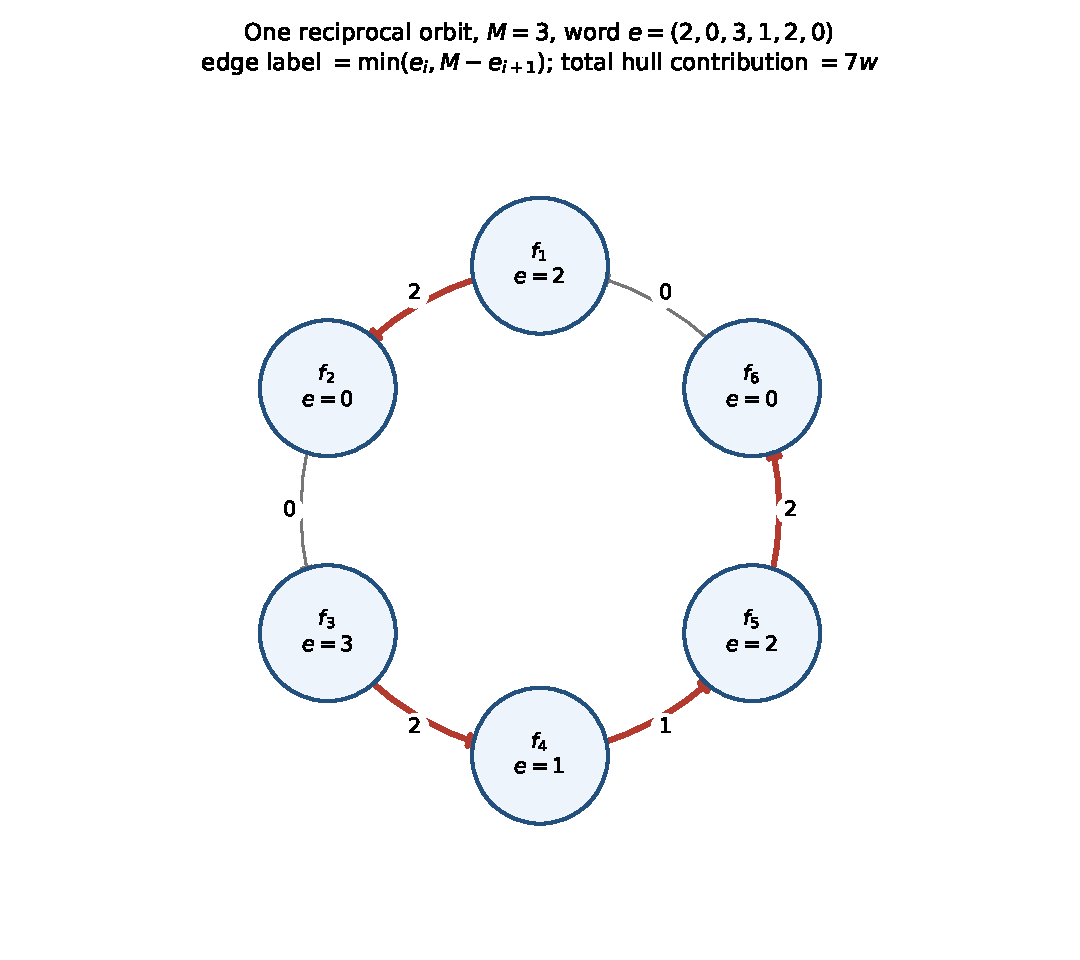
\includegraphics[width=0.72\textwidth]{fig2_orbit_exponent_word.pdf}
\caption{Local cyclic edge-minimum mechanism along a single $\tau_{s,k}$-orbit of
length $a=6$ at multiplicity $M=3$ for the exponent word $e=(2,0,3,1,2,0)$: each
directed edge $f_i\to f_{i+1}$ contributes $w\min\{e_i,M-e_{i+1}\}$, giving total
orbit hull contribution $7w$.}
\label{fig:orbit-word}
\end{figure}

\begin{remark}[Reconciliation with Debnath et al.\ {\cite[Theorem~8]{debnathAffine2026}}]\label{rem:debnath-hull}
In the special case where every component is split over $\F_q$ ($m_s=1$),
$\gcd(\ord(\lambda_s),n')=1$, and every component is compatible
($\ord(\lambda_s)\mid(1+p^{e-k})$), the unshifted identity
$M-\max\{e_{O,i},M-e_{O,i-1}\}=\min\{e_{O,i-1},M-e_{O,i}\}$ in
\eqref{eq:max-to-min} agrees term for term with \cite[Theorem~8]{debnathAffine2026}
(see also Remark~\ref{rem:conventions} regarding their candidate-first pairing).
Writing each summand in the cyclic nearest-neighbour form
$\min\{e_{O,i},M-e_{O,i+1}\}$ has two decisive advantages for enumeration: first,
it holds without any restriction on $m_s\ge 1$ or $\gcd(\ord(\lambda_s),n')$;
second, each term depends only on a directed edge $(e_{O,i},e_{O,i+1})$ along the
cycle $\Z/a_O\Z$, enabling exact transfer-matrix summation over all
$(M+1)^{N_F}$ codes simultaneously.
\end{remark}

\subsection{Transfer matrices and the exact joint enumerator}\label{sec:transfer}

For any unit $\lambda\in\A^*$ and $0\le k<e$, define the exact bivariate
code-dimension and $k$-Galois-hull enumerator and its marginal hull polynomial in
$\Z[U,Z]$ and $\Z[Z]$ by
\begin{equation}\label{eq:enumerator-def}
\Epoly^{(M)}(U,Z):=\sum_{e\in\mathscr C^{(M)}} U^{\kappa(C(e))}\,Z^{\eta_k(C(e))},
\qquad
\Hpoly^{(M)}(Z):=\Epoly^{(M)}(1,Z)=\sum_{e\in\mathscr C^{(M)}} Z^{\eta_k(C(e))}.
\end{equation}
Because $\mathscr C^{(M)}=\prod_{s\in S_{\mathrm{comp}}}\prod_{O\in\Os}
\{0,\dots,M\}^O\times\prod_{s\in S_{\mathrm{inc}}}\{0,\dots,M\}^{\Fs}$ is a
Cartesian product on which both $\kappa(C(e))$ and $\eta_k(C(e))$ in
\eqref{eq:global-code-hull-orbit}--\eqref{eq:global-hull-orbit} decompose
additively with zero cross-terms, the generating sum \eqref{eq:enumerator-def}
factors over all orbits and incompatible factors into independent local sums.

\begin{definition}[Repeated-root transfer matrix]\label{def:transfer-matrix}
For an integer multiplicity $M\ge 1$ and weight $w\ge 1$, the \emph{repeated-root
transfer matrix} $T_w^{(M)}(U,Z)\in\Z[U,Z]^{(M+1)\times(M+1)}$ has rows and
columns indexed by $\alpha,\beta\in\{0,1,\dots,M\}$ in increasing order and
entries
\begin{equation}\label{eq:transfer-entry}
\bigl(T_w^{(M)}(U,Z)\bigr)_{\alpha,\beta}
 :=U^{w(M-\beta)}\,Z^{w\min\{\alpha,\,M-\beta\}}
 \qquad(0\le\alpha,\beta\le M),
\end{equation}
so that $T_w^{(M)}(U,Z)=T_1^{(M)}(U^w,Z^w)$. For $M=1$ and $M=2$ at unit weight
$w=1$, \eqref{eq:transfer-entry} reads explicitly
\begin{equation}\label{eq:T1-T2}
T_1^{(1)}(U,Z)=
\begin{pmatrix}
U & 1 \\
UZ & 1
\end{pmatrix},
\qquad
T_1^{(2)}(U,Z)=
\begin{pmatrix}
U^2 & U & 1 \\
U^2 Z & UZ & 1 \\
U^2 Z^2 & UZ & 1
\end{pmatrix}.
\end{equation}
Figure~\ref{fig:transfer-M2} displays the state-transition entries of
$T_w^{(2)}(U,Z)$ coloured by the edge hull exponent $\min\{\alpha,M-\beta\}$.
\end{definition}

\begin{figure}[htbp]
\centering
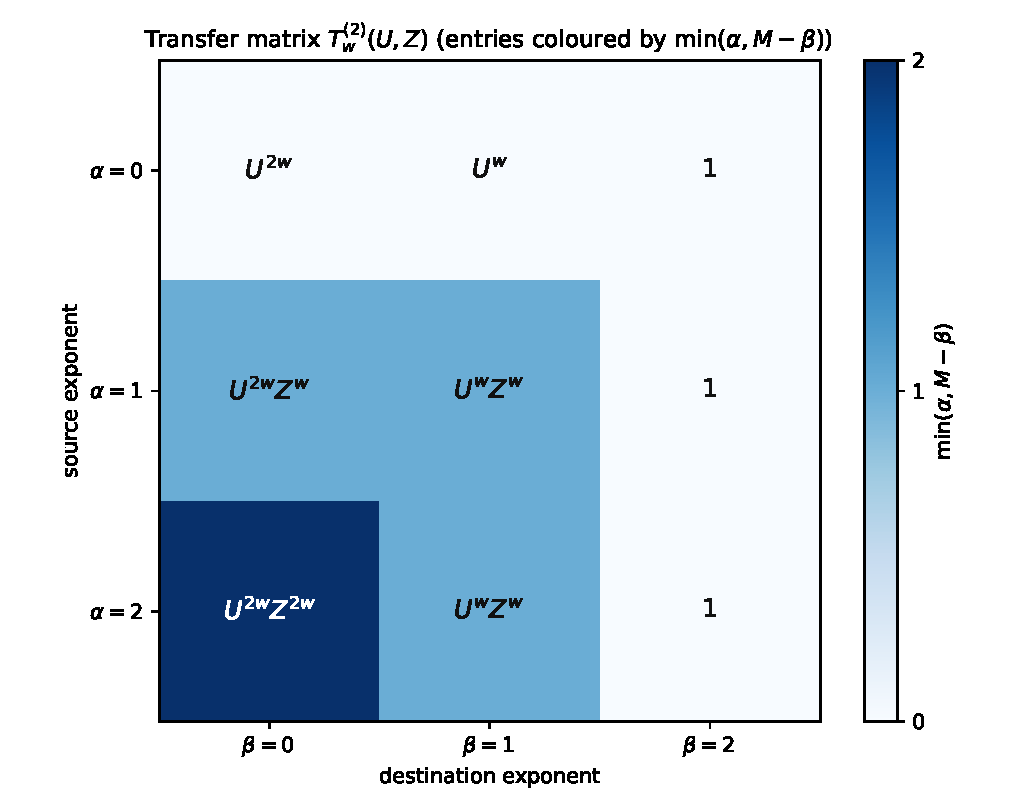
\includegraphics[width=0.68\textwidth]{fig4_transfer_matrix_M2.pdf}
\caption{Structure of the $(M+1)\times(M+1)$ repeated-root transfer matrix
$T_w^{(2)}(U,Z)$ on states $\alpha,\beta\in\{0,1,2\}$, shaded according to the
local hull exponent $\min\{\alpha,2-\beta\}\in\{0,1,2\}$.}
\label{fig:transfer-M2}
\end{figure}

\begin{lemma}[Single-orbit trace formula]\label{lem:orbit-trace}
For every integer $M\ge 1$, orbit length $a\ge 1$, and weight $w\ge 1$, the
single-orbit bivariate enumerator
\[
E_{a,w}^{(M)}(U,Z):=
 \sum_{(e_0,\dots,e_{a-1})\in\{0,\dots,M\}^a}
   U^{w\sum_{i=0}^{a-1}(M-e_i)}\,
   Z^{w\sum_{i=0}^{a-1}\min\{e_i,\,M-e_{i+1}\}}
\]
(with indices taken modulo $a$) satisfies
\begin{equation}\label{eq:orbit-trace}
E_{a,w}^{(M)}(U,Z)=\tr\!\Bigl(T_w^{(M)}(U,Z)^a\Bigr).
\end{equation}
\end{lemma}

\begin{proof}
Expanding the $a$-fold matrix product in $\Z[U,Z]^{(M+1)\times(M+1)}$ and taking
the trace over closed walks $(e_0,e_1,\dots,e_{a-1})\in\{0,\dots,M\}^a$ (with
$e_a:=e_0$) gives
\begin{align*}
\tr\!\Bigl(T_w^{(M)}(U,Z)^a\Bigr)
 &=\sum_{e_0=0}^{M}\sum_{e_1=0}^{M}\cdots\sum_{e_{a-1}=0}^{M}
    \prod_{i=0}^{a-1}\bigl(T_w^{(M)}(U,Z)\bigr)_{e_i,e_{i+1}} \\
 &=\sum_{(e_0,\dots,e_{a-1})\in\{0,\dots,M\}^a}
    U^{w\sum_{i=0}^{a-1}(M-e_{i+1})}\,
    Z^{w\sum_{i=0}^{a-1}\min\{e_i,\,M-e_{i+1}\}}.
\end{align*}
Since $\sum_{i=0}^{a-1}(M-e_{i+1})=\sum_{i=0}^{a-1}(M-e_i)$ around the closed
cycle $e_a=e_0$, this coincides identically with $E_{a,w}^{(M)}(U,Z)$.
\end{proof}

\begin{keyresult}
\begin{theorem}[Exact joint code-dimension and $k$-Galois-hull enumerator]\label{thm:main}
Let $\A\cong\prod_{s=1}^{N}K_s$ be a finite commutative square-free affine
algebra over $\F_q$ ($q=p^e$, $K_s=\F_{q^{m_s}}=\F_{p^{d_s}}$), let $0\le k<e$,
let $n=n'p^t\ge 1$ with $\gcd(n',p)=1$ and $M=p^t$, and let
$\lambda=(\lambda_s)_{s=1}^{N}\in\A^*$ with $M$-th roots $\lambda_{s,0}\in K_s^*$.
Partition $\{1,\dots,N\}=S_{\mathrm{comp}}\sqcup S_{\mathrm{inc}}$ into components
satisfying $\lambda_{s,0}^{\,1+p^{d_s-k}}=1$ and components failing it. Then:
\begin{enumerate}
\item[\textup{(a)}] The exact bivariate enumerator \eqref{eq:enumerator-def} of all
$(M+1)^{N_F}$ labeled $\lambda$-constacyclic codes of length $n$ over $\A$ is
\begin{equation}\label{eq:main-enumerator}
\Epoly^{(M)}(U,Z)
 =\Biggl(\prod_{s\in S_{\mathrm{comp}}}\prod_{O\in\Os}
    \tr\!\Bigl(T_{w_O}^{(M)}(U,Z)^{a_O}\Bigr)\Biggr)
  \Biggl(\prod_{s\in S_{\mathrm{inc}}}\prod_{f\in\Fs}
    \frac{1-U^{(M+1)m_s\deg f}}{1-U^{m_s\deg f}}\Biggr),
\end{equation}
where $a_O=|O|$ and $w_O=m_s\deg f_{O,0}$ for each $\tau_{s,k}$-orbit $O\in\Os$.
\item[\textup{(b)}] When every component is compatible ($S_{\mathrm{inc}}=\emptyset$,
in particular for all cyclic and negacyclic codes), \eqref{eq:main-enumerator}
simplifies to the pure trace product
\begin{equation}\label{eq:main-compatible}
\Epoly^{(M)}(U,Z)=\prod_{s=1}^{N}\prod_{O\in\Os}
 \tr\!\Bigl(T_{w_O}^{(M)}(U,Z)^{a_O}\Bigr),
\qquad
\Hpoly^{(M)}(Z)=\prod_{s=1}^{N}\prod_{O\in\Os}
 \tr\!\Bigl(T_{w_O}^{(M)}(1,Z)^{a_O}\Bigr).
\end{equation}
\end{enumerate}
\end{theorem}
\end{keyresult}

\begin{proof}
Start from Proposition~\ref{prop:incompatible}\textup{(c)}, equation
\eqref{eq:mixed-twists}. On each incompatible component $s\in S_{\mathrm{inc}}$
and each $f\in\Fs$, summing the finite geometric series
$\sum_{r=0}^{M}U^{r m_s\deg f}=(1-U^{(M+1)m_s\deg f})/(1-U^{m_s\deg f})$ yields
the second factor in \eqref{eq:main-enumerator}. On each compatible component
$s\in S_{\mathrm{comp}}$, identify $\{0,\dots,M\}^{\Fs}$ with
$\prod_{O\in\Os}\{0,\dots,M\}^{a_O}$ via $e^{(s)}\mapsto
\bigl((e_{O,0},\dots,e_{O,a_O-1})\bigr)_{O\in\Os}$. Substituting
\eqref{eq:comp-dim} and \eqref{eq:hull-min-component} factors the component sum as
\begin{align*}
\sum_{e^{(s)}\in\{0,\dots,M\}^{\Fs}}
 U^{m_s\dim_{K_s}C_s(e^{(s)})}\,Z^{m_s\dim_{K_s}\Hull_k(C_s(e^{(s)}))}
 &=\prod_{O\in\Os} E_{a_O,w_O}^{(M)}(U,Z) \\
 &=\prod_{O\in\Os}\tr\!\Bigl(T_{w_O}^{(M)}(U,Z)^{a_O}\Bigr),
\end{align*}
where the last equality is Lemma~\ref{lem:orbit-trace}. Specialising
$S_{\mathrm{inc}}=\emptyset$ and $U=1$ gives \eqref{eq:main-compatible}.
\end{proof}

\begin{corollary}[Short orbits and recovery of the simple-root enumerator]\label{cor:short-orbits}
Let $M\ge 1$ and $w\ge 1$.
\begin{enumerate}
\item[\textup{(a)}] \emph{(Self-reciprocal orbits, $a=1$.)}
\begin{equation}\label{eq:orbit-a1}
\tr\!\bigl(T_w^{(M)}(U,Z)\bigr)
 =\sum_{\alpha=0}^{M} U^{w(M-\alpha)}\,Z^{w\min\{\alpha,\,M-\alpha\}}.
\end{equation}
\item[\textup{(b)}] \emph{(Reciprocal pairs, $a=2$.)}
\begin{equation}\label{eq:orbit-a2}
\tr\!\bigl(T_w^{(M)}(U,Z)^2\bigr)
 =\sum_{\alpha=0}^{M}\sum_{\beta=0}^{M}
   U^{w(2M-\alpha-\beta)}\,
   Z^{w\bigl(\min\{\alpha,M-\beta\}+\min\{\beta,M-\alpha\}\bigr)}.
\end{equation}
In particular, writing $x_0:=M-\alpha$ and $x_1:=M-\beta$, every pair with
$x_0+x_1\le M$ satisfies $\min\{\alpha,M-\beta\}+\min\{\beta,M-\alpha\}=x_0+x_1$
(self-orthogonal), while every pair with $x_0+x_1\ge M$ satisfies
$\min\{\alpha,M-\beta\}+\min\{\beta,M-\alpha\}=2M-x_0-x_1$ (dual-containing);
thus on orbits of length $a\in\{1,2\}$ every code attains the upper boundary
$\eta=\min\{\kappa,awM-\kappa\}$.
\item[\textup{(c)}] \emph{(Simple-root specialisation, $M=1$.)} When $t=0$
($\gcd(n,p)=1$, $M=1$), the matrix $T_w^{(1)}(U,Z)=\bigl(\begin{smallmatrix}U^w & 1\\ U^wZ^w & 1\end{smallmatrix}\bigr)$
has trace $1+U^w$ and determinant $U^w(1-Z^w)$, and for every $a\ge 1$,
\begin{equation}\label{eq:M1-binomial}
\tr\!\Bigl(T_w^{(1)}(U,Z)^a\Bigr)=
\begin{cases}
1+U^w, & a=1,\\[4pt]
1+U^{aw}+\displaystyle\sum_{r=1}^{\lfloor a/2\rfloor}\sum_{c=r}^{a-r}
 \frac{a}{r}\binom{c-1}{r-1}\binom{a-c-1}{r-1}U^{wc}Z^{wr}, & a\ge 2.
\end{cases}
\end{equation}
\end{enumerate}
\end{corollary}

\begin{proof}
Parts \textup{(a)} and \textup{(b)} read off the diagonal sums of
$T_w^{(M)}(U,Z)$ and $T_w^{(M)}(U,Z)^2$ directly from \eqref{eq:transfer-entry};
if $x_0+x_1\le M$ then $\alpha=M-x_0\ge x_1=M-\beta$ and $\beta=M-x_1\ge x_0=M-\alpha$,
giving $\min\{\alpha,M-\beta\}+\min\{\beta,M-\alpha\}=x_1+x_0$, and similarly for
$x_0+x_1\ge M$. For \textup{(c)}, setting $M=1$ and $x_i:=1-e_i\in\{0,1\}$ in
Lemma~\ref{lem:orbit-trace} turns $\min\{e_i,1-e_{i+1}\}=\min\{1-x_i,x_{i+1}\}$
into the indicator of a cyclic $0\to 1$ transition $x_i=0,\,x_{i+1}=1$. Around a
cycle of length $a$, the number of $0\to 1$ transitions equals $0$ when $x$ is
constant ($x=0^a$ or $x=1^a$, contributing $1+U^{aw}$) and equals the number
$r\in\{1,\dots,\lfloor a/2\rfloor\}$ of maximal circular runs of $1$s otherwise.
Counting circular binary words of length $a$ with $c$ ones arranged into $r$
circular runs gives $\frac{a}{r}\binom{c-1}{r-1}\binom{a-c-1}{r-1}$~\cite{vanLintWilson2001},
establishing \eqref{eq:M1-binomial}.
\end{proof}

\begin{example}[Full bivariate enumerator for Example~\ref{ex:gate-g1-compatible}]\label{ex:gate-g1-enumerator}
Return to Example~\ref{ex:gate-g1-compatible}: $K_1=\F_4=\F_2(\omega)$, $k=1$,
$n=10=5\cdot 2^1$ ($n'=5$, $M=2$), $\lambda_{1,0}=\omega$, $\lambda_1=\omega^2$,
where $\tau_{1,1}$ has one self-reciprocal orbit $O_1=(f_1)$ with $(a_1,w_1)=(1,1)$
and one reciprocal pair $O_2=(f_2,f_3)$ with $(a_2,w_2)=(2,2)$. By
Corollary~\ref{cor:short-orbits}\textup{(a)}--\textup{(b)},
\[
\tr\!\bigl(T_1^{(2)}(U,Z)\bigr)=1+UZ+U^2,
\qquad
\tr\!\bigl(T_2^{(2)}(U,Z)^2\bigr)=1+2U^2Z^2+3U^4Z^4+2U^6Z^2+U^8.
\]
Multiplying these two local traces as in Theorem~\ref{thm:main}\textup{(b)} gives
all $3^3=27$ constacyclic codes in $15$ distinct $(\kappa,\eta_1)$ classes:
\begin{align*}
\Epoly^{(2)}(U,Z)
 &=1+UZ+U^2+2U^2Z^2+2U^3Z^3+2U^4Z^2+3U^4Z^4+3U^5Z^5 \\
 &\quad +2U^6Z^2+3U^6Z^4+2U^7Z^3+U^8+2U^8Z^2+U^9Z+U^{10}.
\end{align*}
Setting $Z=0$ leaves $1+U^2+U^8+U^{10}$ ($4$ $1$-Galois LCD codes, equal to
$2^{|\mathcal O_1|}=2^2$), while the central term $3U^5Z^5$ counts three
$1$-Galois self-dual codes arising from the midpoint exponent $e_{f_1}=M/2=1$ on
$O_1$ paired with the three solutions of $e_{f_2}+e_{f_3}=2$ on $O_2$ — a
strictly repeated-root phenomenon absent at simple-root length $n'=5$, where odd
ambient dimension precludes self-dual codes altogether.
\end{example}

\section{Consequences}\label{sec:consequences}

Theorem~\ref{thm:main} reduces global questions across all $(M+1)^{N_F}$
repeated-root constacyclic codes to explicit algebraic operations on the local
$(M+1)\times(M+1)$ transfer matrices $T_w^{(M)}(U,Z)$. We derive in turn the
univariate marginals and global duality symmetry (\S\ref{sec:marginals}), the
multiplicity invariance of $k$-Galois LCD codes (\S\ref{sec:lcd}), the exact
single-orbit support trapezoid and attainable hull spectrum (\S\ref{sec:support}),
exact unconditional and conditional moments (\S\ref{sec:moments}), and closed
enumerators for self-orthogonal, dual-containing, and self-dual codes
(\S\ref{sec:extremal}).

\subsection{Marginals and global duality symmetry}\label{sec:marginals}

\begin{proposition}[Marginals and duality reflection]\label{prop:marginals}
Let $\lambda\in\A^*$ be any unit, $0\le k<e$, $n=n'p^t$, $M=p^t$, and
$W=n\sum_{s=1}^{N}m_s$.
\begin{enumerate}
\item[\textup{(a)}] Setting $Z=1$ eliminates all $k$-dependence: each row of
$T_w^{(M)}(U,1)$ is $(U^{wM},U^{w(M-1)},\dots,1)$, a rank-$1$ matrix of
trace $\sum_{r=0}^{M}U^{rw}$, and
\begin{equation}\label{eq:code-marginal}
\Epoly^{(M)}(U,1)
 =\prod_{s=1}^{N}\prod_{f\in\Fs}\frac{1-U^{(M+1)m_s\deg f}}{1-U^{m_s\deg f}},
\qquad
\Epoly^{(M)}(1,1)=\Hpoly^{(M)}(1)=(M+1)^{N_F}.
\end{equation}
\item[\textup{(b)}] The bivariate enumerator satisfies the global functional equation
\begin{equation}\label{eq:duality-symmetry}
U^W\,\Epoly^{(M)}\!\bigl(U^{-1},Z\bigr)=\Epoly^{(M)}(U,Z),
\end{equation}
so $[U^\kappa Z^\eta]\Epoly^{(M)}(U,Z)=[U^{W-\kappa}Z^\eta]\Epoly^{(M)}(U,Z)$ for
all $0\le\kappa\le W$ and all $\eta\ge 0$.
\end{enumerate}
\end{proposition}

\begin{proof}
At $Z=1$, $\tr(T_w^{(M)}(U,1)^a)=(\tr T_w^{(M)}(U,1))^a=(\sum_{r=0}^{M}U^{rw})^a$,
and substituting this into \eqref{eq:main-enumerator} combines $S_{\mathrm{comp}}$
and $S_{\mathrm{inc}}$ into \eqref{eq:code-marginal}; setting $U=1$ evaluates each
factor at $M+1$, yielding $(M+1)^{\sum_s|\Fs|}=(M+1)^{N_F}$.

For \textup{(b)}, on each orbit $O\in\Os$ of length $a=a_O$, define the involution
$\iota:\{0,\dots,M\}^a\to\{0,\dots,M\}^a$ by cyclic reversal and complementation,
$(\iota(e))_i:=M-e_{-i}$ ($i\in\Z/a\Z$). Then
$\sum_{i=0}^{a-1}(M-(\iota(e))_i)=\sum_{i=0}^{a-1}e_{-i}=aM-\sum_{i=0}^{a-1}(M-e_i)$,
while the hull statistic is preserved termwise up to reversal:
\[
\sum_{i=0}^{a-1}\min\bigl\{(\iota(e))_i,\,M-(\iota(e))_{i+1}\bigr\}
 =\sum_{i=0}^{a-1}\min\{M-e_{-i},\,e_{-i-1}\}
 =\sum_{j=0}^{a-1}\min\{e_j,\,M-e_{j+1}\}
\]
via $j=-i-1\in\Z/a\Z$. Thus $U^{awM}E_{a,w}^{(M)}(U^{-1},Z)=E_{a,w}^{(M)}(U,Z)$.
On each $f\in\Fs$ with $s\in S_{\mathrm{inc}}$, substituting $r'=M-r$ gives
$U^{Mm_s\deg f}\sum_{r=0}^{M}U^{-rm_s\deg f}=\sum_{r'=0}^{M}U^{r'm_s\deg f}$.
Multiplying across all orbits and incompatible factors and noting
$\sum_{s\in S_{\mathrm{comp}}}\sum_{O\in\Os}a_O w_O M
+\sum_{s\in S_{\mathrm{inc}}}\sum_{f\in\Fs}m_s(\deg f)M=W$ yields
\eqref{eq:duality-symmetry}.
\end{proof}

\subsection{Multiplicity invariance of \texorpdfstring{$k$}{k}-Galois LCD codes}\label{sec:lcd}

\begin{keyresult}
\begin{theorem}[Characterisation and $p$-power invariance of $k$-Galois LCD codes]\label{thm:lcd-invariance}
Let $\lambda\in\A^*$ have partition $\{1,\dots,N\}=S_{\mathrm{comp}}\sqcup
S_{\mathrm{inc}}$, and let $n=n'p^t$ with $\gcd(n',p)=1$ and $M=p^t\ge 1$.
\begin{enumerate}
\item[\textup{(a)}] \emph{(Generator characterisation.)} An exponent selection
$e=(e^{(s)})_{s=1}^{N}\in\mathscr C^{(M)}$ defines a $k$-Galois LCD code
($\Hull_{\A,k}(C(e))=\{0\}$) if and only if for every compatible component
$s\in S_{\mathrm{comp}}$ and every $\tau_{s,k}$-orbit $O\in\Os$, the restriction
of $e^{(s)}$ to $O$ is constant at an extreme value:
\[
\text{either }\; e_f=0\text{ for all }f\in O
\quad\text{or}\quad
e_f=M\text{ for all }f\in O,
\]
equivalently $g_{e^{(s)}}(x)=g_{s,0}(x)^M$ where $\langle g_{s,0}(x)\rangle$ is a
simple-root $k$-Galois LCD $\lambda_{s,0}$-constacyclic code of length $n'$ over
$K_s$, while $e^{(s)}\in\{0,\dots,M\}^{\Fs}$ is arbitrary for $s\in S_{\mathrm{inc}}$.
\item[\textup{(b)}] \emph{(LCD generating polynomial and Jordan structure.)} The
code-dimension enumerator of all $k$-Galois LCD $\lambda$-constacyclic codes is
\begin{equation}\label{eq:lcd-enumerator}
\Epoly^{(M)}(U,0)
 =\Biggl(\prod_{s\in S_{\mathrm{comp}}}\prod_{O\in\Os}\bigl(1+U^{Ma_Ow_O}\bigr)\Biggr)
  \Biggl(\prod_{s\in S_{\mathrm{inc}}}\prod_{f\in\Fs}
    \frac{1-U^{(M+1)m_s\deg f}}{1-U^{m_s\deg f}}\Biggr).
\end{equation}
Moreover, the unweighted $(M+1)\times(M+1)$ LCD transition matrix
$L_M:=T_1^{(M)}(1,0)$ with entries $(L_M)_{\alpha,\beta}=\mathbf 1_{\{\alpha=0
\text{ or }\beta=M\}}$ has rank $2$ for every $M\ge 1$, characteristic polynomial
$\det(tI_{M+1}-L_M)=t^{M-1}(t-1)^2$, Jordan block
$\bigl(\begin{smallmatrix}1 & M\\ 0 & 1\end{smallmatrix}\bigr)$ on its
$2$-dimensional image, and $\tr(L_M^a)=2$ for all $M\ge 1$ and $a\ge 1$.
\item[\textup{(c)}] \emph{(Purely compatible $p$-power invariance.)} Whenever
$S_{\mathrm{inc}}=\emptyset$ (in particular for all cyclic and negacyclic codes
over $\A$), the total number of $k$-Galois LCD $\lambda$-constacyclic codes of
length $n=n'p^t$ over $\A$ is
\begin{equation}\label{eq:lcd-count}
\Hpoly^{(M)}(0)=\Epoly^{(M)}(1,0)=2^{\sum_{s=1}^{N}|\Os|},
\end{equation}
completely independent of $t=v_p(n)\ge 0$, whereas the uniform probability that a
random $\lambda$-constacyclic code is $k$-Galois LCD equals
$2^{\sum_{s=1}^{N}|\Os|}(p^t+1)^{-N_F}$.
\end{enumerate}
\end{theorem}
\end{keyresult}

\begin{proof}
By \eqref{eq:global-hull-orbit}, $\eta_k(C(e))=0$ if and only if
$\min\{e_{O,i},M-e_{O,i+1}\}=0$ for every $s\in S_{\mathrm{comp}}$, every
$O\in\Os$, and every $i\in\Z/a_O\Z$. On a fixed cycle of length $a=a_O$, the
condition $\min\{e_i,M-e_{i+1}\}=0$ reads: whenever $e_i\ge 1$, one must have
$e_{i+1}=M$. Hence if $e_{i_0}\ge 1$ for at least one index $i_0\in\Z/a\Z$,
iterating $a$ times forces $e_{i_0+1}=M\ge 1$, $e_{i_0+2}=M\ge 1$, and so on,
giving $e_i=M$ for all $i\in\Z/a\Z$; otherwise $e_i=0$ for all $i\in\Z/a\Z$.
Conversely, both constant words $0^a$ and $M^a$ give $\min\{e_i,M-e_{i+1}\}=0$
everywhere and contribute $U^{aw_OM}$ and $1$ respectively to $\Epoly^{(M)}(U,0)$,
proving \textup{(a)} and \eqref{eq:lcd-enumerator}.

For the spectral statement in \textup{(b)}, write $v_1:=e_0=(1,0,\dots,0)^{\mathsf T}$
and $v_2:=\sum_{\beta=1}^{M}e_\beta=(0,1,\dots,1)^{\mathsf T}$ in $\mathbb Q^{M+1}$.
Columns $0,\dots,M-1$ of $L_M$ all equal $v_1$ and column $M$ equals $v_1+v_2$, so
$\operatorname{im}(L_M)=\operatorname{span}\{v_1,v_2\}$ has dimension $2$,
$\dim\ker(L_M)=M-1$, $L_M v_1=v_1$, and
$L_M v_2=(M-1)v_1+(v_1+v_2)=Mv_1+v_2$. Thus $L_M$ acts as
$\bigl(\begin{smallmatrix}1 & M\\ 0 & 1\end{smallmatrix}\bigr)$ on
$\operatorname{span}\{v_1,v_2\}$ and nilpotently ($0$) on a supplement, yielding
$\det(tI_{M+1}-L_M)=t^{M-1}(t-1)^2$ and $\tr(L_M^a)=1^a+1^a=2$. Evaluating
\eqref{eq:lcd-enumerator} at $U=1$ with $S_{\mathrm{inc}}=\emptyset$ gives
\eqref{eq:lcd-count} and the stated density inside $|\mathscr C^{(M)}|=(p^t+1)^{N_F}$.
\end{proof}

\begin{remark}\label{rem:pang-chen}
At $N=1$, $m_1=1$, $\lambda=1$, and $k=0$, Theorem~\ref{thm:lcd-invariance}\textup{(c)}
recovers the repeated-root Euclidean cyclic LCD count over $\F_q$ of Pang, Zhu,
and Li~\cite{pangZhuLi2018} (and at $n=2\ell^m p^t$, $k=0$ aligns with
Chen, Dinh, and Liu~\cite{chenDinhLiu2015}), while extending it simultaneously to
arbitrary $k$-Galois pairings, general constacyclic twists (showing that
incompatibility switches the scaling from $2^{|\Os|}$ to $(p^t+1)^{|\Fs|}$),
non-split square-free affine algebras $\A$, and the full bivariate distribution
around $\eta_k=0$ illustrated in Figure~\ref{fig:hull-marginals}.
\end{remark}

\begin{figure}[htbp]
\centering
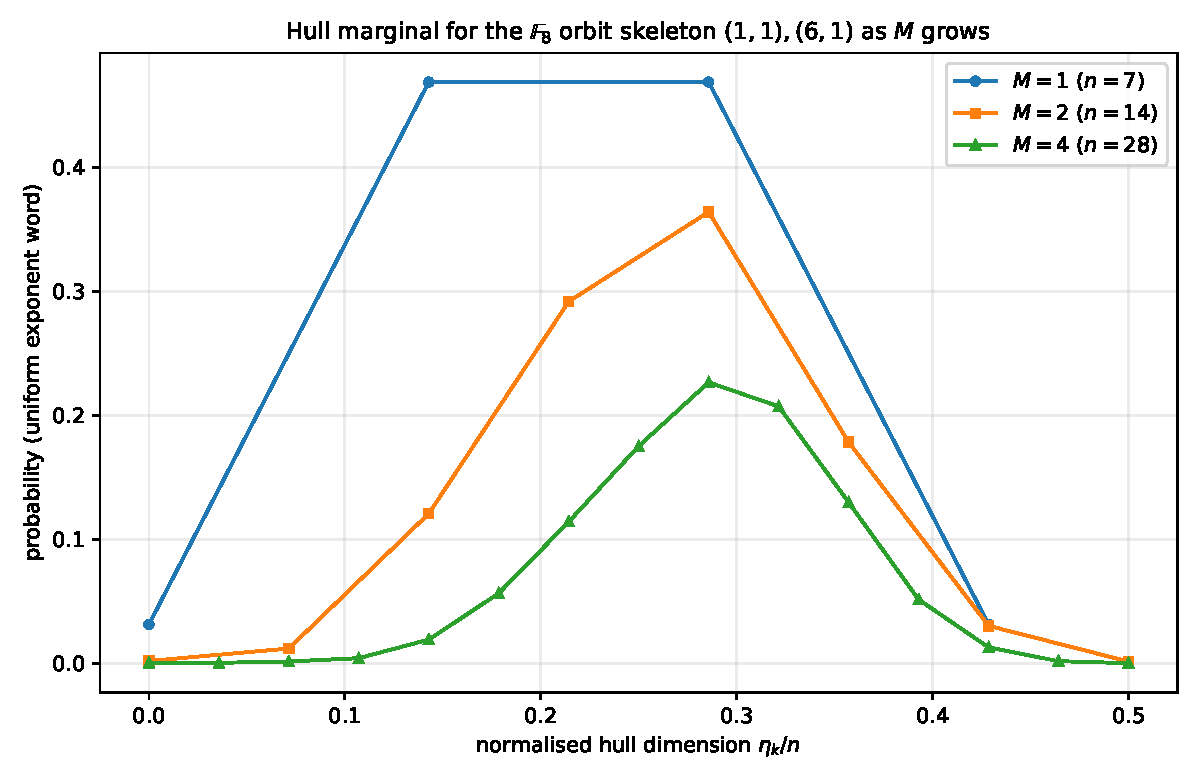
\includegraphics[width=0.78\textwidth]{fig7_hull_marginals.pdf}
\caption{Evolution of the normalised marginal $1$-Galois hull distribution
$\mathbb P(\eta_1(C)=\eta)$ versus $\eta/n$ along the $2$-power multiplicity tower
$M=1,2,4$ ($n=7,14,28$) for the cyclic $\F_8$ orbit skeleton $(1,1),(6,1)$: while
the absolute LCD count at $\eta=0$ stays locked at $2^2=4$ across all $M$, probability
mass concentrates steadily around the asymptotic mean ratio $\eta/n\approx 19/63$
($M=2$) and $\to 13/42$ as $M\to\infty$.}
\label{fig:hull-marginals}
\end{figure}

\subsection{Exact single-orbit support trapezoid and hull spectrum}\label{sec:support}

\begin{keyresult}
\begin{theorem}[Exact single-orbit support trapezoid]\label{thm:support-trapezoid}
For every multiplicity $M\ge 1$, orbit length $a\ge 1$, and weight $w\ge 1$, the
support of the single-orbit enumerator $E_{a,w}^{(M)}(U,Z)=\tr(T_w^{(M)}(U,Z)^a)$
is the exact lattice polygon
\begin{equation}\label{eq:support-trapezoid}
\operatorname{Supp}\bigl(E_{a,w}^{(M)}\bigr)
 =\Bigl\{(wR,wH)\in\Z_{\ge 0}^2:
    0\le R\le aM,\;
    \min\{R,M,aM-R\}\le H\le\min\{R,aM-R\}\Bigr\}.
\end{equation}
In particular, the number of nonzero monomials in $E_{a,w}^{(M)}(U,Z)$ equals
\begin{equation}\label{eq:support-cardinality}
\bigl|\operatorname{Supp}(E_{a,w}^{(M)})\bigr|=
\begin{cases}
M+1, & a=1,\\[4pt]
aM+1+\left\lfloor\dfrac{(a-2)^2 M^2}{4}\right\rfloor, & a\ge 2.
\end{cases}
\end{equation}
\end{theorem}
\end{keyresult}

\begin{proof}
Scaling by $w$ reduces to $w=1$. Put $x_i:=M-e_i\in\{0,\dots,M\}$ ($i\in\Z/a\Z$),
so $R(x):=\sum_{i=0}^{a-1}x_i\in\{0,\dots,aM\}$ and
$H(x):=\sum_{i=0}^{a-1}\min\{M-x_i,\,x_{i+1}\}$. For $a=1$, $R=x_0$ and
$H=\min\{M-R,R\}=\min\{R,M,M-R\}$, giving both \eqref{eq:support-trapezoid} and
cardinality $M+1$. For $a=2$, Corollary~\ref{cor:short-orbits}\textup{(b)} gives
$H(x_0,x_1)=\min\{R,2M-R\}=\min\{R,M,2M-R\}$ for every $0\le R\le 2M$, yielding
\eqref{eq:support-trapezoid} and cardinality $2M+1=2M+1+\lfloor 0/4\rfloor$.

Assume henceforth that $a\ge 3$. For the upper bound, summing the inequalities
$\min\{M-x_i,x_{i+1}\}\le x_{i+1}$ and $\min\{M-x_i,x_{i+1}\}\le M-x_i$ around
$\Z/a\Z$ gives $H(x)\le\min\{R(x),\,aM-R(x)\}$.

For the lower bound $H(x)\ge\min\{R(x),\,M,\,aM-R(x)\}$, note first that the
reversal-complement involution $\tilde{x}_i:=M-x_{-i}$ satisfies
$R(\tilde{x})=aM-R(x)$, $H(\tilde{x})=H(x)$, $\min_i\tilde{x}_i=M-\max_i x_i$,
and $\max_i\tilde{x}_i=M-\min_i x_i$. Replacing $x$ by $\tilde{x}$ if necessary,
we may assume $x_{\min}+x_{\max}\le M$, where $x_{\min}:=\min_i x_i$ and
$x_{\max}:=\max_i x_i$. Write each edge minimum as the threshold sum (illustrated
in Figure~\ref{fig:threshold-layers})
\[
\min\{M-x_i,\,x_{i+1}\}
 =\sum_{r=1}^{M}\mathbf 1_{\{x_i\le M-r\;\text{and}\;x_{i+1}\ge r\}}.
\]
If $x_{\max}\le\lfloor M/2\rfloor$, then $x_i+x_{i+1}\le 2x_{\max}\le M$ for all
$i$, so $\min\{M-x_i,x_{i+1}\}=x_{i+1}$ everywhere and $H(x)=R(x)$. Suppose
instead that $x_{\max}\ge\lfloor M/2\rfloor+1$, set $K:=M-x_{\max}\in
\{0,\dots,\lfloor(M-1)/2\rfloor\}$, and choose vertices $p,q\in\Z/a\Z$ with
$x_p=x_{\min}\le K$ and $x_q=x_{\max}=M-K$.
\begin{itemize}
\item For every $1\le r\le K$, we have $x_i\le x_{\max}=M-K\le M-r$ for all $i$,
so the $r$-th threshold sum around $\Z/a\Z$ equals $\#\{i:x_{i+1}\ge r\}$; summing
over $1\le r\le K$ contributes $\sum_{i=0}^{a-1}\min\{x_i,K\}$.
\item Pair each remaining integer $K+1\le r\le\lfloor M/2\rfloor$ with
$r':=M+1-r>r$, partitioning $\Z/a\Z$ into $L^{(r)}:=\{i:x_i\le r-1\}$,
$C^{(r)}:=\{i:r\le x_i\le M-r\}$, and $H^{(r)}:=\{i:x_i\ge M+1-r\}$. Because
$x_p\le K\le r-1$ and $x_q=M-K\ge M+1-r$, both $L^{(r)}$ and $H^{(r)}$ are
non-empty. Subtracting the zero cycle sum of $\Phi^{(r)}(x_{i+1})-\Phi^{(r)}(x_i)$
with $\Phi^{(r)}:=\mathbf 1_{H^{(r)}}$, the paired edge weight
$c_r(i):=\mathbf 1_{\{x_i\le M-r,\,x_{i+1}\ge r\}}+\mathbf 1_{\{x_i\le r-1,\,x_{i+1}\ge M+1-r\}}$
satisfies $c_r(i)-(\Phi^{(r)}(x_{i+1})-\Phi^{(r)}(x_i))\ge 0$ on all nine state
transitions, equals $+1$ on every exit from $H^{(r)}$ ($H^{(r)}\to L^{(r)}\cup C^{(r)}$),
equals $+1$ on $L^{(r)}\to H^{(r)}$, and equals $+1$ on $L^{(r)}\to C^{(r)}$.
Since $L^{(r)}$ and $H^{(r)}$ are both non-empty, traversing $\Z/a\Z$ leaves
$H^{(r)}$ at least once ($+1$) and re-enters $H^{(r)}$ from $L^{(r)}$ either
directly ($L^{(r)}\to H^{(r)}$, $+1$) or via $C^{(r)}$ preceded by
$L^{(r)}\to C^{(r)}$ ($+1$), forcing $\sum_{i=0}^{a-1}c_r(i)\ge 2$. If $M$ is odd,
the unpaired middle threshold $r=(M+1)/2$ likewise has non-empty $L^{(r)}$ and
$H^{(r)}$ ($C^{(r)}=\emptyset$), forcing at least one $L^{(r)}\to H^{(r)}$ edge
($+1$).
\end{itemize}
Combining all levels gives
\[
H(x)\ge\sum_{i=0}^{a-1}\min\{x_i,K\}+2\bigl(\lfloor M/2\rfloor-K\bigr)+(M\bmod 2)
    =(M-2K)+\sum_{i=0}^{a-1}\min\{x_i,K\}.
\]
Separating vertex $q$ (where $\min\{x_q,K\}=K$) rewrites the right-hand side as
$(M-K)+\sum_{i\neq q}\min\{x_i,K\}$. If $x_i\le K$ for all $i\neq q$ this equals
$x_q+\sum_{i\neq q}x_i=R(x)$; if $x_{i_1}\ge K$ for at least one $i_1\neq q$ it
is at least $(M-K)+K=M$. In every case $H(x)\ge\min\{R(x),M,aM-R(x)\}$.

It remains to show that every integer $H\in[\min\{R,M,aM-R\},\,\min\{R,aM-R\}]$ is
attained for fixed $0\le R\le aM$. By symmetry we may assume $R\le\lfloor aM/2\rfloor$.
If $R\le M$, the interval reduces to $\{R\}$, attained by $x=(R,0,\dots,0)$. Suppose
$M<R\le\lfloor aM/2\rfloor$. Write $R=q_0 M+r_0$ with $q_0\ge 1$, $0\le r_0<M$;
since $R<aM$, the packed vector $x^{\min}:=(M,\dots,M,r_0,0,\dots,0)\in\{0,\dots,M\}^a$
has at least one zero coordinate and satisfies $H(x^{\min})=M$ (only the closing
$0\to M$ edge contributes $M$). Define capacities
$\mathrm{cap}_i:=\lfloor M/2\rfloor+\mathbf 1_{\{M\text{ odd},\,i\text{ even},\,i<a-1\}}$
for $0\le i<a$. Readily $\sum_{i=0}^{a-1}\mathrm{cap}_i=\lfloor aM/2\rfloor\ge R$
and $\mathrm{cap}_i+\mathrm{cap}_{i+1}\le M$ for all $i\in\Z/a\Z$, so choosing any
$x^{\max}\in\{0,\dots,M\}^a$ with $0\le x^{\max}_i\le\mathrm{cap}_i$ and
$\sum_i x^{\max}_i=R$ gives $x^{\max}_i+x^{\max}_{i+1}\le M$ everywhere and hence
$H(x^{\max})=R$.

Now transform $x^{\min}$ into $x^{\max}$ along the path $0\text{--}1\text{--}\cdots\text{--}(a-1)$
by elementary adjacent unit transfers $(x_j,x_{j+1})\mapsto(x_j\mp 1,x_{j+1}\pm 1)$
preserving $x\in\{0,\dots,M\}^a$: matching coordinates from left to right, whenever $x_u>x^{\max}_u$ let $r>u$ be
minimal with $x_r<M$ and slide one unit across $(r-1\to r),\dots,(u\to u+1)$,
and symmetrically via the minimal $r>u$ with $x_r>0$ when $x_u<x^{\max}_u$. Because $a\ge 3$, vertices $j-1,j,j+1$ are
distinct at every single step $(x_j,x_{j+1})\mapsto(x_j-1,x_{j+1}+1)$, and the
three affected circular edges change by
\begin{align*}
\Delta H
 &=\Bigl(\min\{M-x_{j-1},x_j-1\}-\min\{M-x_{j-1},x_j\}\Bigr) \\
 &\quad +\Bigl(\min\{M-x_j+1,x_{j+1}+1\}-\min\{M-x_j,x_{j+1}\}\Bigr) \\
 &\quad +\Bigl(\min\{M-x_{j+1}-1,x_{j+2}\}-\min\{M-x_{j+1},x_{j+2}\}\Bigr) \\
 &\in\{-1,0\}+\{+1\}+\{-1,0\}=\{-1,0,+1\}.
\end{align*}
Since $H$ starts at $M$, ends at $R$, and changes by at most $1$ at every step,
every integer in $[M,R]$ is attained along the walk, proving \eqref{eq:support-trapezoid}.

Finally, summing slice heights $\min\{R,aM-R\}-\min\{R,M,aM-R\}+1
=1+(\min\{R,aM-R\}-M)_+$ over $0\le R\le aM$ gives $aM+1+\sum_{s=0}^{L}\min\{s,L-s\}$
with $L:=(a-2)M$, and $\sum_{s=0}^{L}\min\{s,L-s\}=\lfloor L^2/4\rfloor$ yields
\eqref{eq:support-cardinality} (cf.\ Figure~\ref{fig:support-trapezoid}).
\end{proof}

\begin{figure}[htbp]
\centering
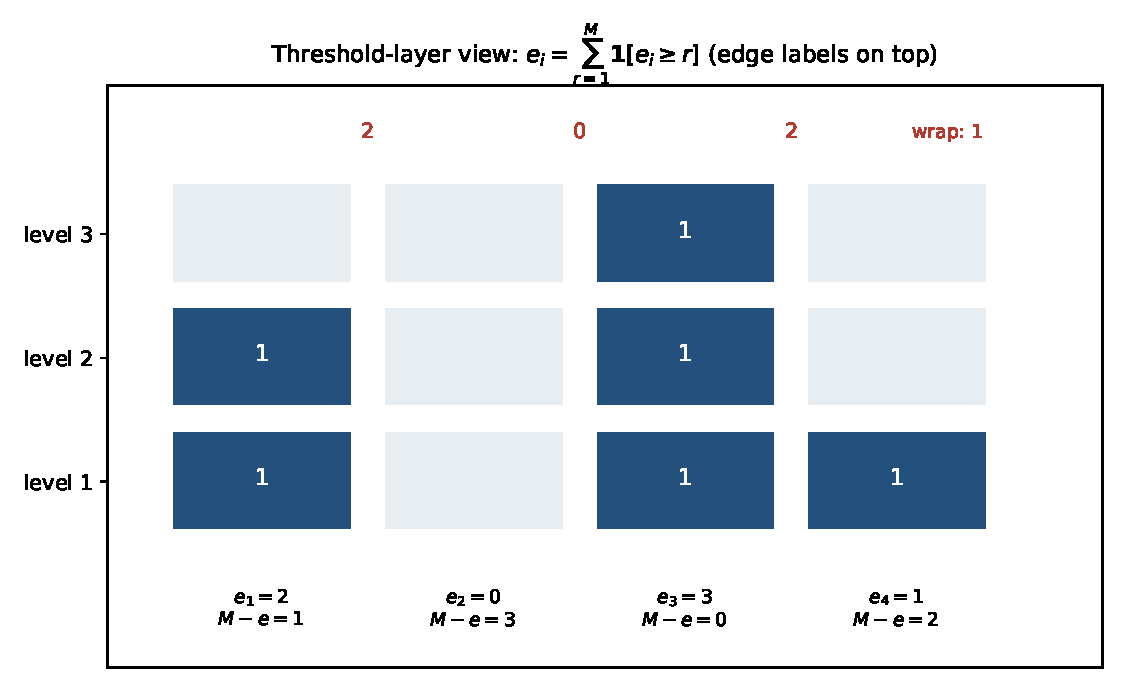
\includegraphics[width=0.75\textwidth]{fig3_threshold_layers.pdf}
\caption{Binary threshold-layer decomposition $e_i=\sum_{r=1}^{M}\mathbf 1_{\{e_i\ge r\}}$
underlying the lower-bound proof of Theorem~\ref{thm:support-trapezoid}, shown for
$a=4$, $M=3$, and $e=(2,0,3,1)$ with cyclic edge contributions $(2,0,2,1)$.}
\label{fig:threshold-layers}
\end{figure}

\begin{figure}[htbp]
\centering
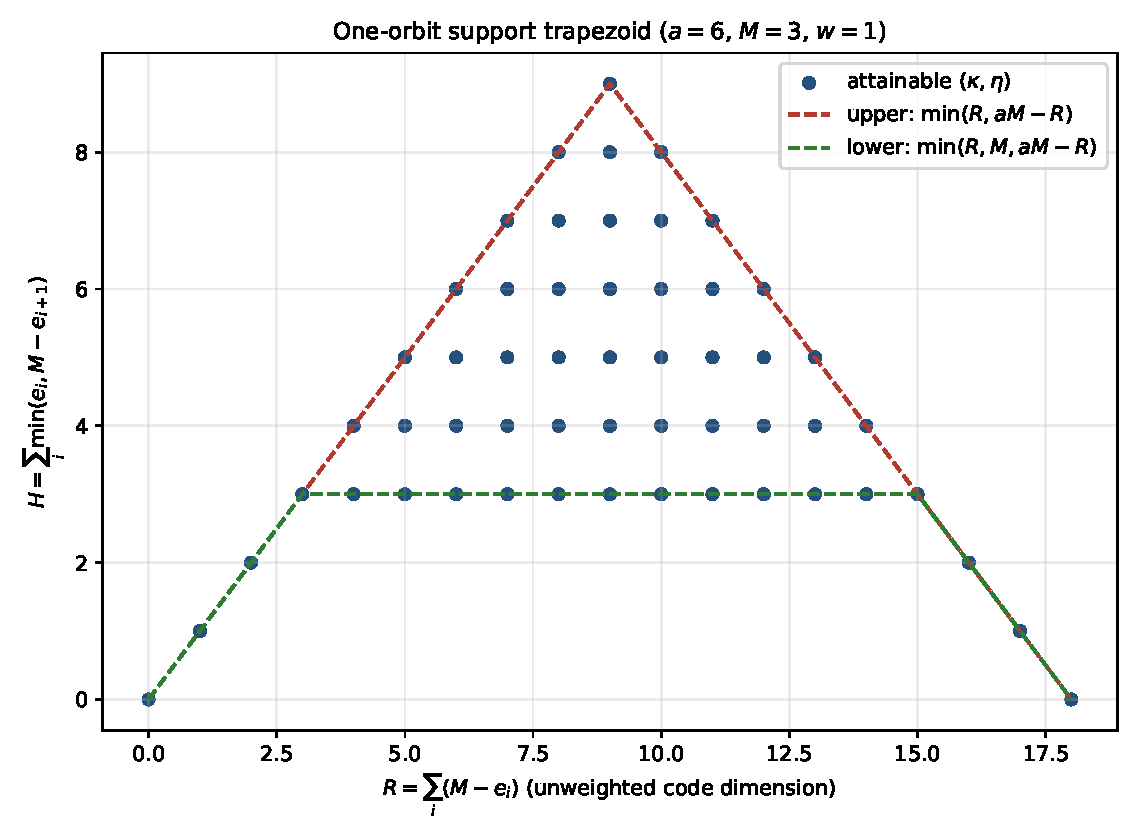
\includegraphics[width=0.76\textwidth]{fig8_support_trapezoid.pdf}
\caption{Exact single-orbit support polygon $\operatorname{Supp}(E_{6,1}^{(3)})$
for $a=6$, $M=3$, $w=1$: every lattice point $(R,H)$ between the lower floor
$\min\{R,3,18-R\}$ (green dashed) and upper tent $\min\{R,18-R\}$ (red dashed) is
attained, giving $6\cdot 3+1+\lfloor 4^2\cdot 3^2/4\rfloor=55$ distinct monomials.}
\label{fig:support-trapezoid}
\end{figure}

\begin{corollary}[Global attainable $k$-Galois hull spectrum]\label{cor:hull-spectrum}
For any unit $\lambda\in\A^*$ and $0\le k<e$, the set of $\F_q$-dimensions
attained by $\Hull_{\A,k}(C)$ as $C$ ranges over all $\lambda$-constacyclic codes
of length $n=n'p^t$ ($M=p^t$) over $\A$ is the Minkowski sum
\begin{equation}\label{eq:global-hull-spectrum}
\Bigl\{\eta_k(C):C\in\mathscr C^{(M)}\Bigr\}
 =\sum_{s\in S_{\mathrm{comp}}}\sum_{O\in\Os}
   w_O\cdot\bigl\{0,1,\dots,\lfloor a_O M/2\rfloor\bigr\},
\end{equation}
understood as $\{0\}$ when $S_{\mathrm{comp}}=\emptyset$. In particular,
$\max_{C}\eta_k(C)=\sum_{s\in S_{\mathrm{comp}}}\sum_{O\in\Os}
w_O\lfloor a_O M/2\rfloor$.
\end{corollary}

\begin{proof}
Because every coefficient of $\tr(T_{w_O}^{(M)}(1,Z)^{a_O})$ is a non-negative
integer, the support of the product \eqref{eq:main-enumerator} at $U=1$ is the
Minkowski sum of the supports of its factors. On each single orbit $(a_O,w_O)$,
projecting \eqref{eq:support-trapezoid} onto the second coordinate gives
$\bigcup_{R=0}^{a_O M}[w_O\min\{R,M,a_O M-R\},\,w_O\min\{R,a_O M-R\}]
=w_O\{0,1,\dots,\lfloor a_O M/2\rfloor\}$, because $R=0,1,\dots,\min\{M,\lfloor a_O M/2\rfloor\}$
covers $\{0,\dots,\min\{M,\lfloor a_O M/2\rfloor\}\}$ while $R=\lfloor a_O M/2\rfloor$
covers $[\min\{M,\lfloor a_O M/2\rfloor\},\,\lfloor a_O M/2\rfloor]$.
\end{proof}

\subsection{Exact moments, zero global covariance, and conditional laws}\label{sec:moments}

\begin{keyresult}
\begin{theorem}[Exact mean, variance, and covariance of $(\kappa,\eta_k)$]\label{thm:moments}
Endow $\mathscr C^{(M)}$ with the uniform measure $\mathbb P(C(e))=(M+1)^{-N_F}$,
and write $M=p^t\ge 1$.
\begin{enumerate}
\item[\textup{(a)}] \emph{(Code dimension and global covariance.)}
\begin{equation}\label{eq:kappa-moments-cov}
\mathbb E[\kappa]=\frac{W}{2},
\qquad
\Var(\kappa)=\frac{M(M+2)}{12}\sum_{s=1}^{N}\sum_{f\in\Fs} m_s^2(\deg f)^2,
\qquad
\Cov(\kappa,\eta_k)=0.
\end{equation}
\item[\textup{(b)}] \emph{(Hull mean and variance across all orbit lengths.)}
\begin{equation}\label{eq:eta-mean}
\mathbb E[\eta_k]
 =\sum_{s\in S_{\mathrm{comp}}}\Biggl(
    \sum_{\substack{O\in\Os\\ a_O=1}} w_O\,\frac{\lfloor M^2/4\rfloor}{M+1}
   +\sum_{\substack{O\in\Os\\ a_O\ge 2}} a_O w_O\,\frac{M(2M+1)}{6(M+1)}
  \Biggr),
\end{equation}
and
\begin{equation}\label{eq:eta-variance}
\Var(\eta_k)=\sum_{s\in S_{\mathrm{comp}}}\sum_{O\in\Os} w_O^2\,\mathcal V_M(a_O),
\end{equation}
where the unweighted orbit variance function $\mathcal V_M(a)$ is given cleanly
across the three correlation regimes $a=1$, $a=2$, and $a\ge 3$ by
\begin{equation}\label{eq:orbit-variance-regimes}
\mathcal V_M(a)=
\begin{cases}
\dfrac{M(M+2)(M^2+2M+4)}{48(M+1)^2}, & a=1,\;M\text{ even},\\[9pt]
\dfrac{(M-1)(M+3)}{48}, & a=1,\;M\text{ odd},\\[9pt]
\dfrac{M(M+2)(M^2+2M+3)}{18(M+1)^2}, & a=2,\\[9pt]
\dfrac{a\,M(M+2)(M^2+2M+2)}{60(M+1)^2}, & a\ge 3.
\end{cases}
\end{equation}
\end{enumerate}
At $M=1$ ($t=0$), \eqref{eq:eta-mean}--\eqref{eq:orbit-variance-regimes} reduce to
the simple-root variance constants $\mathcal V_1(1)=0$, $\mathcal V_1(2)=1/4$,
and $\mathcal V_1(a)=a/16$ ($a\ge 3$). As $M=p^t\to\infty$ with fixed
coprime part $n'$, the normalised mean satisfies
\[
\lim_{t\to\infty}\frac{\mathbb E[\eta_k]}{M}
 =\sum_{s\in S_{\mathrm{comp}}}\Biggl(
    \frac{1}{4}\sum_{\substack{O\in\Os\\ a_O=1}} w_O
   +\frac{1}{3}\sum_{\substack{O\in\Os\\ a_O\ge 2}} a_O w_O
  \Biggr).
\]
\end{theorem}
\end{keyresult}

\begin{proof}
Under the uniform measure on $\mathscr C^{(M)}$, the random exponents
$(e_f)_{f\in\bigsqcup_s\Fs}$ are independent and uniformly distributed on
$\{0,1,\dots,M\}$. Since $\mathbb E[M-e_f]=M/2$ and
$\Var(M-e_f)=M(M+2)/12$, linearity and independence in \eqref{eq:global-dim} yield
$\mathbb E[\kappa]$ and $\Var(\kappa)$. By Proposition~\ref{prop:marginals}\textup{(b)},
$(\kappa,\eta_k)\stackrel{d}{=}(W-\kappa,\eta_k)$, whence
$\mathbb E[\kappa\eta_k]=\mathbb E[(W-\kappa)\eta_k]=W\mathbb E[\eta_k]-\mathbb E[\kappa\eta_k]$,
so $\mathbb E[\kappa\eta_k]=\frac{W}{2}\mathbb E[\eta_k]=\mathbb E[\kappa]\mathbb E[\eta_k]$
and $\Cov(\kappa,\eta_k)=0$.

Because distinct orbits are independent, both $\mathbb E[\eta_k]$ and
$\Var(\eta_k)$ split additively over $O\in\Os$. Let $X,Y,Z'\stackrel{\mathrm{i.i.d.}}{\sim}
\mathrm{Unif}\{0,\dots,M\}$ and put $g(u,v):=\min\{u,M-v\}$.
\begin{itemize}
\item \emph{Regime $a=1$:} $Y_1:=g(X,X)=\min\{X,M-X\}$ takes values
$0,1,\dots,r-1$ twice each and $r$ once when $M=2r$ is even, and values
$0,1,\dots,r$ twice each when $M=2r+1$ is odd. Direct summation of $\sum x$ and
$\sum x^2$ gives $\mathbb E[Y_1]=\lfloor M^2/4\rfloor/(M+1)$ and the two parity
formulas for $\mathcal V_M(1)=\Var(Y_1)$ in \eqref{eq:orbit-variance-regimes}.
\item \emph{Single-edge moments ($a\ge 2$):} For $1\le r\le M$,
$\#\{(u,v)\in\{0,\dots,M\}^2:g(u,v)\ge r\}=(M+1-r)^2$. Summing $1$ and $2r-1$
against $(M+1-r)^2$ over $1\le r\le M$ gives
\begin{gather*}
\mathbb E[g(X,Y)]=\frac{M(2M+1)}{6(M+1)},
\qquad
\mathbb E[g(X,Y)^2]=\frac{M(M^2+M+1)}{6(M+1)},\\[4pt]
\Var\bigl(g(X,Y)\bigr)=\frac{M(M+2)(2M^2+4M+3)}{36(M+1)^2}.
\end{gather*}
Summing $\mathbb E[g(X_i,X_{i+1})]$ around $i\in\Z/a\Z$ gives \eqref{eq:eta-mean}.
\item \emph{Regime $a=2$:} Direct summation over $0\le x,y\le M$ yields
$\sum_{x,y=0}^{M}g(x,y)g(y,x)=M^2(M-1)(M+1)/12$, so
$\Cov(g(X,Y),g(Y,X))=-M^2(M+2)^2/\bigl(36(M+1)^2\bigr)$ and
\[
\mathcal V_M(2)=2\Bigl(\Var(g(X,Y))+\Cov\bigl(g(X,Y),g(Y,X)\bigr)\Bigr)
 =\frac{M(M+2)(M^2+2M+3)}{18(M+1)^2}.
\]
\item \emph{Regime $a\ge 3$:} Along the cycle $(X_0,\dots,X_{a-1})$ with $a\ge 3$,
edges $g(X_i,X_{i+1})$ and $g(X_j,X_{j+1})$ share no variables (hence have zero
covariance) whenever $j\notin\{i-1,i,i+1\}$ modulo $a$, while each of the $a$
adjacent pairs $(g(X,Y),g(Y,Z'))$ satisfies, upon conditioning on $c:=M-Y\in\{0,\dots,M\}$,
\[
\sum_{x=0}^{M}g(x,Y)=\frac{c(2M+1-c)}{2},
\qquad
\sum_{z=0}^{M}g(Y,z)=\frac{(M-c)(M+1+c)}{2},
\]
whence $\mathbb E[g(X,Y)g(Y,Z')]=M(M-1)(11M^2+15M+6)/\bigl(120(M+1)^2\bigr)$
(vanishing at $M=1$ because $g(X,Y)=1$ forces $Y=0$ whereas $g(Y,Z')=1$ forces
$Y=1$) and
\[
\Cov\bigl(g(X,Y),g(Y,Z')\bigr)=-\frac{M(M+2)(7M^2+14M+9)}{360(M+1)^2}.
\]
Note that adjacent edges are strictly negatively correlated for every $M\ge 1$.
Therefore
\[
\mathcal V_M(a)=a\Bigl(\Var(g(X,Y))+2\Cov\bigl(g(X,Y),g(Y,Z')\bigr)\Bigr)
 =\frac{a\,M(M+2)(M^2+2M+2)}{60(M+1)^2}.\qedhere
\]
\end{itemize}
\end{proof}

Table~\ref{tab:moment-coeffs} records exact rational values of the local moment
constants across representative prime powers $M=p^t$.

\begin{table}[htbp]
\centering
\caption{Exact unweighted local expectation, covariance, and variance constants across prime-power multiplicities $M=p^t$ (Theorem~\ref{thm:moments}).}
\label{tab:moment-coeffs}
\scriptsize
\setlength{\tabcolsep}{4pt}
\begin{tabular}{@{}rrrrrrrr@{}}
\toprule
$M$ & $\mathbb E[g]$ ($a\ge 2$) & $\mathbb E[Y_1]$ ($a=1$) & $\Var(g)$ & $\Cov_{\mathrm{adj}}$ & $\mathcal V_M(a)/a$ ($a\ge 3$) & $\mathcal V_M(2)$ & $\mathcal V_M(1)$ \\
\midrule
$1$  & $1/4$     & $0$       & $3/16$        & $-1/16$        & $1/16$        & $1/4$         & $0$ \\
$2$  & $5/9$     & $1/3$     & $38/81$       & $-13/81$       & $4/27$        & $44/81$       & $2/9$ \\
$3$  & $7/8$     & $1/2$     & $55/64$       & $-19/64$       & $17/64$       & $15/16$       & $1/4$ \\
$4$  & $6/5$     & $4/5$     & $34/25$       & $-59/125$      & $52/125$      & $36/25$       & $14/25$ \\
$5$  & $55/36$   & $1$       & $2555/1296$   & $-889/1296$    & $259/432$     & $665/324$     & $2/3$ \\
$8$  & $68/27$   & $16/9$    & $3260/729$    & $-1138/729$    & $328/243$     & $3320/729$    & $140/81$ \\
$9$  & $57/20$   & $2$       & $2211/400$    & $-3861/2000$   & $3333/2000$   & $561/100$     & $2$ \\
$16$ & $88/17$   & $64/17$   & $4632/289$    & $-1620/289$    & $1392/289$    & $4656/289$    & $1752/289$ \\
$25$ & $425/52$  & $6$       & $101475/2704$ & $-35505/2704$  & $30465/2704$  & $25425/676$   & $14$ \\
$27$ & $495/56$  & $13/2$    & $136503/3136$ & $-47763/3136$  & $40977/3136$  & $34191/784$   & $65/4$ \\
$32$ & $1040/99$ & $256/33$  & $592688/9801$ & $-207400/9801$ & $59296/3267$  & $593504/9801$ & $24752/1089$ \\
\bottomrule
\end{tabular}
\end{table}

Although $\Cov(\kappa,\eta_k)=0$ globally, $\eta_k$ depends strongly and
concavely on the code dimension $\kappa$, as captured exact slice by slice via
factorial-moment extraction (Figure~\ref{fig:conditional-F32}).

\begin{proposition}[Exact conditional moments given code dimension]\label{prop:conditional}
For $j\in\{0,1,2\}$ and $0\le\kappa\le W$, put
$\Phi_j(\kappa):=[U^\kappa]\,\partial_Z^j\Epoly^{(M)}(U,Z)\big|_{Z=1}$. Whenever
$\Phi_0(\kappa)>0$,
\begin{equation}\label{eq:conditional-moments}
\mathbb E[\eta_k\mid\kappa(C)=\kappa]=\frac{\Phi_1(\kappa)}{\Phi_0(\kappa)},
\qquad
\Var(\eta_k\mid\kappa(C)=\kappa)
 =\frac{\Phi_2(\kappa)+\Phi_1(\kappa)}{\Phi_0(\kappa)}
  -\left(\frac{\Phi_1(\kappa)}{\Phi_0(\kappa)}\right)^2,
\end{equation}
and both functions satisfy the reflection identity
$F(W-\kappa)=F(\kappa)$ for all attainable $\kappa$. Moreover, $\Phi_0,\Phi_1,\Phi_2$
are determined without forming full bivariate polynomials by evaluating
\eqref{eq:main-enumerator} in the truncated jet ring
$\Z[U][Z]/\langle(Z-1)^3\rangle$.
\end{proposition}

\begin{proof}
Differentiating $\Epoly^{(M)}(U,Z)=\sum_{\kappa,\eta}N_{\kappa,\eta}U^\kappa Z^\eta$
$j$ times with respect to $Z$ at $Z=1$ gives $\Phi_0(\kappa)=\sum_\eta N_{\kappa,\eta}$,
$\Phi_1(\kappa)=\sum_\eta\eta N_{\kappa,\eta}$, and
$\Phi_2(\kappa)=\sum_\eta\eta(\eta-1)N_{\kappa,\eta}$, from which
\eqref{eq:conditional-moments} follows via $\eta^2=\eta(\eta-1)+\eta$. Symmetry in
$\kappa\leftrightarrow W-\kappa$ follows by differentiating \eqref{eq:duality-symmetry}
at $Z=1$, and expanding $Z=1+\varepsilon\pmod{\varepsilon^3}$ yields
$\Epoly^{(M)}(U,1+\varepsilon)\equiv\sum_\kappa\bigl(\Phi_0(\kappa)
+\Phi_1(\kappa)\varepsilon+\frac{1}{2}\Phi_2(\kappa)\varepsilon^2\bigr)U^\kappa$.
\end{proof}

\begin{figure}[htbp]
\centering
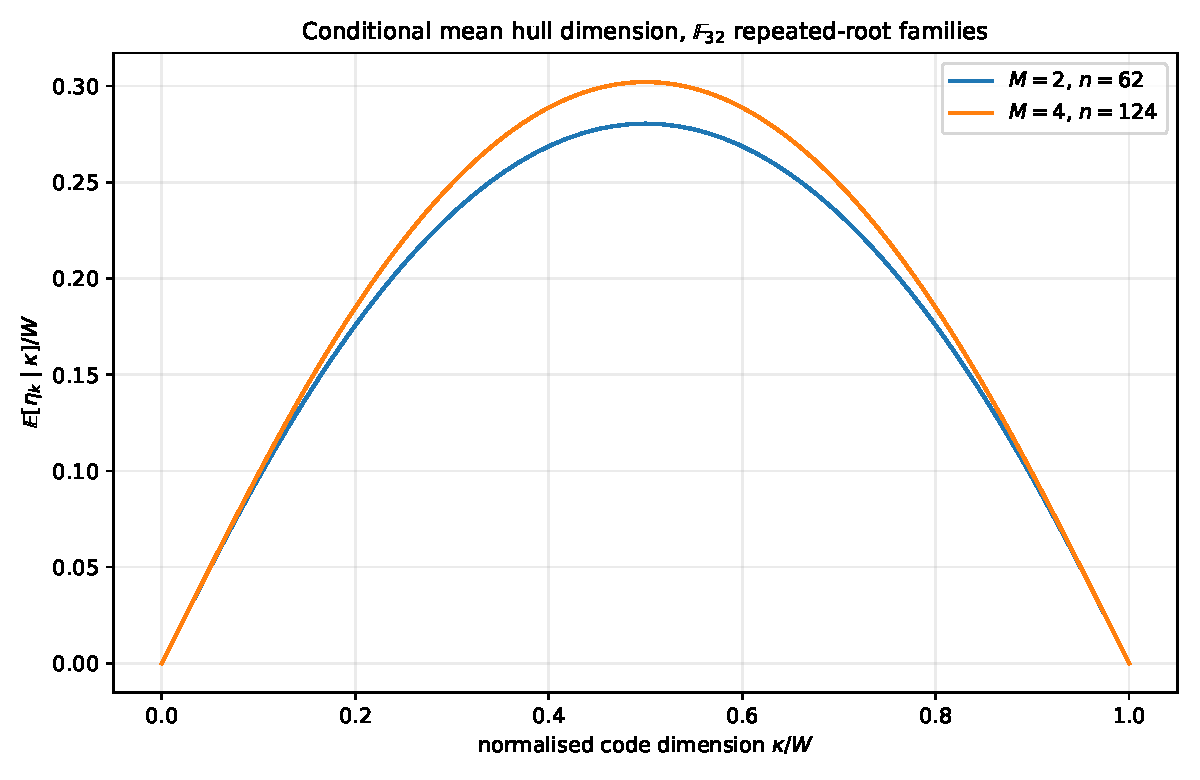
\includegraphics[width=0.76\textwidth]{fig9_conditional_F32.pdf}
\caption{Exact conditional expectation $\mathbb E[\eta_1\mid\kappa]/W$ versus
normalised rate $\kappa/W$ for cyclic codes over $\F_{32}$ at repeated-root
lengths $n=62$ ($M=2$, $3^{31}\approx 6.18\times 10^{14}$ codes) and $n=124$
($M=4$, $5^{31}\approx 4.66\times 10^{21}$ codes), symmetric around $\kappa/W=1/2$
with global linear covariance $\Cov(\kappa,\eta_1)=0$.}
\label{fig:conditional-F32}
\end{figure}

\subsection{Self-orthogonal, dual-containing, and self-dual code counts}\label{sec:extremal}

\begin{theorem}[Enumeration of extremal $k$-Galois duality classes]\label{thm:extremal}
For $M\ge 1$, define $(M+1)\times(M+1)$ $\{0,1\}$-matrices on $\{0,\dots,M\}$ by
\[
\bigl(A_{\mathrm{SO}}^{(M)}\bigr)_{\alpha,\beta}:=\mathbf 1_{\{\alpha+\beta\ge M\}},
\qquad
\bigl(A_{\mathrm{DC}}^{(M)}\bigr)_{\alpha,\beta}:=\mathbf 1_{\{\alpha+\beta\le M\}},
\qquad
\bigl(A_{\mathrm{SD}}^{(M)}\bigr)_{\alpha,\beta}:=\mathbf 1_{\{\alpha+\beta=M\}}.
\]
Let $\lambda\in\A^*$ have partition $\{1,\dots,N\}=S_{\mathrm{comp}}\sqcup S_{\mathrm{inc}}$.
\begin{enumerate}
\item[\textup{(a)}] The numbers $N_{\mathrm{SO}}^{(M)}$ of $k$-Galois
self-orthogonal codes ($C\subseteq D_{\A,k}(C)$, equivalently $\eta_k(C)=\kappa(C)$)
and $N_{\mathrm{DC}}^{(M)}$ of $k$-Galois dual-containing codes
($D_{\A,k}(C)\subseteq C$, equivalently $\eta_k(C)=W-\kappa(C)$) satisfy
\begin{equation}\label{eq:SO-DC-counts}
N_{\mathrm{SO}}^{(M)}=N_{\mathrm{DC}}^{(M)}
 =\prod_{s\in S_{\mathrm{comp}}}\prod_{O\in\Os}
   \tr\!\Bigl(\bigl(A_{\mathrm{SO}}^{(M)}\bigr)^{a_O}\Bigr),
\end{equation}
and their $\F_q$-dimension enumerators equal $[t^0]\,\Epoly^{(M)}(Ut,t^{-1})$ and
$[t^W]\,\Epoly^{(M)}(Ut,t)$ respectively. For $a_O=1$ and $a_O=2$,
$\tr(A_{\mathrm{SO}}^{(M)})=\lceil(M+1)/2\rceil$ and
$\tr\bigl((A_{\mathrm{SO}}^{(M)})^2\bigr)=\binom{M+2}{2}$, while at $M=1$ the
traces $\tr\bigl((A_{\mathrm{SO}}^{(1)})^a\bigr)=L_a$ ($L_1=1$, $L_2=3$,
$L_a=L_{a-1}+L_{a-2}$) reproduce the classical Lucas numbers.
\item[\textup{(b)}] The number $N_{\mathrm{SD}}^{(M)}$ of $k$-Galois self-dual
$\lambda$-constacyclic codes ($C=D_{\A,k}(C)$, equivalently
$\kappa(C)=\eta_k(C)=W/2$) is given in closed form by
\begin{equation}\label{eq:SD-count}
N_{\mathrm{SD}}^{(M)}=
\begin{cases}
0, & \text{if }S_{\mathrm{inc}}\neq\emptyset\text{ or }\bigl(M\text{ is odd and }\exists\,O\in\bigsqcup_{s\in S_{\mathrm{comp}}}\Os\text{ with }a_O\text{ odd}\bigr),\\[6pt]
(M+1)^{\#\{(s,O)\,:\,s\in S_{\mathrm{comp}},\,O\in\Os,\,a_O\text{ even}\}}, & \text{otherwise}.
\end{cases}
\end{equation}
In particular, passing to repeated roots $t\ge 1$ in characteristic $p=2$ ($M=2^t$
even) unlocks self-dual constacyclic codes whenever self-reciprocal or odd-length
orbits exist on compatible components, whereas in odd characteristic $p\ge 3$
($M=p^t$ odd) odd-length orbits remain a permanent obstruction for every $t\ge 0$.
\end{enumerate}
\end{theorem}

\begin{proof}
Since $\Hull_{\A,k}(C)=C\cap D_{\A,k}(C)$ and $\dim_{\F_q}D_{\A,k}(C)=W-\kappa(C)$,
we have $C\subseteq D_{\A,k}(C)\iff\eta_k(C)=\kappa(C)$,
$D_{\A,k}(C)\subseteq C\iff\eta_k(C)=W-\kappa(C)$, and
$C=D_{\A,k}(C)\iff\eta_k(C)=\kappa(C)=W/2$, yielding the generating-function
extractions from $\Epoly^{(M)}(U,Z)$. Directly at the generator level,
Proposition~\ref{prop:incompatible}\textup{(b)} pins every $s\in S_{\mathrm{inc}}$
to the unique choice $e_f=M$ for self-orthogonality ($1$ factor), $e_f=0$ for
dual containment ($1$ factor), and $0$ choices for self-duality. On each
$s\in S_{\mathrm{comp}}$, comparing exponents in \eqref{eq:gen-check} and
\eqref{eq:dual-gen-compatible} shows that $C_s(e)\subseteq\Dk(C_s(e))$ holds if
and only if $M-e_{O,i-1}\le e_{O,i}$, i.e.\ $e_{O,i-1}+e_{O,i}\ge M$, along every
orbit $O\in\Os$, counted by $\tr\bigl((A_{\mathrm{SO}}^{(M)})^{a_O}\bigr)$.
Conjugating $A_{\mathrm{SO}}^{(M)}$ by the permutation involution
$J:=A_{\mathrm{SD}}^{(M)}$ ($J_{\alpha,\beta}=\delta_{\alpha,M-\beta}$) gives
$J A_{\mathrm{SO}}^{(M)} J=A_{\mathrm{DC}}^{(M)}$, proving
$\tr\bigl((A_{\mathrm{SO}}^{(M)})^{a_O}\bigr)=\tr\bigl((A_{\mathrm{DC}}^{(M)})^{a_O}\bigr)$
and \eqref{eq:SO-DC-counts}. For $a=1$, $\#\{\alpha\in\{0,\dots,M\}:2\alpha\ge M\}
=\lceil(M+1)/2\rceil$; for $a=2$, $\#\{(\alpha,\beta):\alpha+\beta\ge M\}
=\sum_{r=0}^{M}(r+1)=\binom{M+2}{2}$.

Finally, self-duality on orbit $O$ holds if and only if $e_{O,i-1}+e_{O,i}=M$ for
all $i\in\Z/a_O\Z$, counted by $\tr(J^{a_O})$. Since $J^2=I_{M+1}$, $\tr(J^{a_O})=M+1$
when $a_O$ is even, while when $a_O$ is odd $\tr(J^{a_O})=\tr(J)
=\#\{\alpha:2\alpha=M\}=\mathbf 1_{\{M\text{ even}\}}$, giving \eqref{eq:SD-count}.
\end{proof}

Table~\ref{tab:one-orbit-extremal} lists exact single-orbit counts across
$1\le M\le 5$ and representative orbit lengths $a$.

\begin{table}[htbp]
\centering
\caption{Exact single-orbit counts of total codes $(M+1)^a$, LCD codes, self-orthogonal / dual-containing codes ($N_{\mathrm{SO}}=N_{\mathrm{DC}}$), and self-dual codes across $1\le M\le 5$ (Theorems~\ref{thm:lcd-invariance} and \ref{thm:extremal}).}
\label{tab:one-orbit-extremal}
\footnotesize
\begin{tabular}{@{}rrrrrr@{\hspace{2.2em}}rrrrrr@{}}
\toprule
$a$ & $M$ & $(M+1)^a$ & LCD & SO / DC & SD & $a$ & $M$ & $(M+1)^a$ & LCD & SO / DC & SD \\
\midrule
$1$ & $1$ & $2$    & $2$ & $1$   & $0$ & $4$  & $1$ & $16$       & $2$ & $7$       & $2$ \\
$1$ & $2$ & $3$    & $2$ & $2$   & $1$ & $4$  & $2$ & $81$       & $2$ & $26$      & $3$ \\
$1$ & $3$ & $4$    & $2$ & $2$   & $0$ & $4$  & $3$ & $256$      & $2$ & $70$      & $4$ \\
$1$ & $4$ & $5$    & $2$ & $3$   & $1$ & $4$  & $4$ & $625$      & $2$ & $155$     & $5$ \\
$1$ & $5$ & $6$    & $2$ & $3$   & $0$ & $4$  & $5$ & $1296$     & $2$ & $301$     & $6$ \\
\addlinespace[2pt]
$2$ & $1$ & $4$    & $2$ & $3$   & $2$ & $5$  & $1$ & $32$       & $2$ & $11$      & $0$ \\
$2$ & $2$ & $9$    & $2$ & $6$   & $3$ & $5$  & $2$ & $243$      & $2$ & $57$      & $1$ \\
$2$ & $3$ & $16$   & $2$ & $10$  & $4$ & $5$  & $3$ & $1024$     & $2$ & $197$     & $0$ \\
$2$ & $4$ & $25$   & $2$ & $15$  & $5$ & $5$  & $4$ & $3125$     & $2$ & $533$     & $1$ \\
$2$ & $5$ & $36$   & $2$ & $21$  & $6$ & $5$  & $5$ & $7776$     & $2$ & $1223$    & $0$ \\
\addlinespace[2pt]
$3$ & $1$ & $8$    & $2$ & $4$   & $0$ & $6$  & $1$ & $64$       & $2$ & $18$      & $2$ \\
$3$ & $2$ & $27$   & $2$ & $11$  & $1$ & $6$  & $2$ & $729$      & $2$ & $129$     & $3$ \\
$3$ & $3$ & $64$   & $2$ & $23$  & $0$ & $6$  & $3$ & $4096$     & $2$ & $571$     & $4$ \\
$3$ & $4$ & $125$  & $2$ & $42$  & $1$ & $6$  & $4$ & $15625$    & $2$ & $1884$    & $5$ \\
$3$ & $5$ & $216$  & $2$ & $69$  & $0$ & $10$ & $5$ & $60466176$ & $2$ & $1508401$ & $6$ \\
\bottomrule
\end{tabular}
\end{table}

\section{Computation and examples}\label{sec:examples}

We next translate Theorem~\ref{thm:main} and Proposition~\ref{prop:conditional}
into exact polynomial-time dynamic-programming algorithms (\S\ref{sec:algorithm}),
document our independent linear-algebraic and quotient-ring verification suite
(\S\ref{sec:verification}), and analyse benchmark code families spanning
characteristics $p\in\{2,3,5\}$, non-cyclic twists, non-split affine algebras,
and state spaces exceeding $4.6\times 10^{21}$ codes (\S\ref{sec:benchmarks}).

\subsection{Dynamic-programming evaluation and arithmetic complexity}\label{sec:algorithm}

Brute-force enumeration over $\mathscr C^{(M)}$ inspects $(M+1)^{N_F}$ codes,
which is exponential in both $N_F$ and $t=v_p(n)$. By contrast,
\eqref{eq:main-enumerator} computes $\Epoly^{(M)}(U,Z)$ without listing individual
codes.

\begin{proposition}[Polynomial-time dynamic programming for $\Epoly^{(M)}(U,Z)$]\label{prop:algorithm}
Given the orbit multisets $\{(a_O,w_O):O\in\Os\}$ ($s\in S_{\mathrm{comp}}$) and
factor degrees $\{\deg f:f\in\Fs\}$ ($s\in S_{\mathrm{inc}}$), with ambient
dimension $W=n\sum_{s=1}^{N}m_s$ and multiplicity $M=p^t$:
\begin{enumerate}
\item[\textup{(a)}] \emph{(Full bivariate table.)} Initialising $G(U,Z):=1$ and,
for each compatible orbit $(a_O,w_O)$, summing over initial states
$s_0\in\{0,\dots,M\}$ the $a_O$-step DP array $S_r[u]$ ($0\le r\le a_O$,
$0\le u\le M$) updated by
\[
S_{r+1}[\beta]\;\mathrel{+}=\;
 U^{w_O(M-\beta)}\,Z^{w_O\min\{\alpha,\,M-\beta\}}\,S_r[\alpha]
 \qquad(0\le\alpha,\beta\le M),
\]
followed by $f$-wise multiplication across $s\in S_{\mathrm{inc}}$, computes all
nonzero coefficients of $\Epoly^{(M)}(U,Z)$ in
\begin{equation}\label{eq:dp-complexity}
O\!\Bigl(M^3\sum_{s\in S_{\mathrm{comp}}} a_O\cdot |\mathcal S_{\max}|\Bigr)
 =O\!\bigl(M^3 N_F W^2\bigr)
\end{equation}
operations on exact $O(N_F\log M)$-bit integers, where
$|\mathcal S_{\max}|\le(W+1)(\lfloor W/2\rfloor+1)=O(W^2)$ bounds the intermediate
support size. Alternatively, binary exponentiation of $T_{w_O}^{(M)}(U,Z)^{a_O}$
evaluates each single-orbit trace in $O(\log a_O)$ polynomial-matrix multiplications
on $(M+1)\times(M+1)$ matrices.
\item[\textup{(b)}] \emph{(Truncated $3$-jet for conditional moments.)} Carrying
coefficients in $\Z[U][Z]/\langle(Z-1)^3\rangle$ replaces bivariate tables of size
$O(W^2)$ by triples of degree-$\le W$ univariate polynomials, computing
$\Phi_0(\kappa),\Phi_1(\kappa),\Phi_2(\kappa)$ for all $0\le\kappa\le W$ in
$O(M^3 N_F W)$ integer operations.
\end{enumerate}
\end{proposition}

\begin{proof}
Fix an orbit $(a,w)$. For each pinned start state $s_0\in\{0,\dots,M\}$, induction
on $r=0,\dots,a$ shows that $S_r[u]$ equals $\sum U^{w\sum_{i=1}^{r}(M-e_i)}
Z^{w\sum_{i=0}^{r-1}\min\{e_i,M-e_{i+1}\}}G(U,Z)$ summed over walks
$s_0=e_0\to e_1\to\dots\to e_r=u$. Extracting $S_a[s_0]$ and summing over all
$M+1$ choices of $s_0$ multiplies $G(U,Z)$ by $\tr(T_w^{(M)}(U,Z)^a)$ by
Lemma~\ref{lem:orbit-trace}. Each of the $\sum_O a_O\le N_F$ transitions executes
$(M+1)$ start states $\times\,(M+1)^2$ pairs $(\alpha,\beta)$ across at most
$|\mathcal S_{\max}|$ nonzero $(\kappa,\eta)$ entries, giving \eqref{eq:dp-complexity}.
In $\Z[U][Z]/\langle(Z-1)^3\rangle$, only three $Z$-jet coordinates exist per
$\kappa\in\{0,\dots,W\}$, reducing $|\mathcal S_{\max}|$ from $O(W^2)$ to $3(W+1)=O(W)$.
\end{proof}

\subsection{Independent linear-algebraic and quotient-ring verification}\label{sec:verification}

To guard against any hidden algebra, indexing, or parity error, every formula in
Sections~\ref{sec:duality}--\ref{sec:consequences} was cross-checked by an
independent standard-library Python verification suite (\texttt{verify\_rr.py})
requiring zero input from transfer matrices or orbit combinatorics:
\begin{enumerate}
\item \emph{Arbitrary-degree Cantor--Zassenhaus factorisation and Gram-rank
verification.} Over explicit prime-extension fields $K_s=\F_{p^d}$ across
$p\in\{2,3,5\}$, $x^{n'}-\lambda_{s,0}$ is factored from scratch by
distinct-degree and Cantor--Zassenhaus splitting (covering linear, quadratic,
cubic, and quartic irreducibles). For every exponent tuple $e$, the monic
divisor $g_e(x)$ is expanded directly in $K_s[x]$, a $(\dim_{K_s}C)\times n$ shift
generator matrix $B$ is formed in $K_s^n$, and $\dim_{K_s}\Hull_k(C_s(e))$ is
computed directly from $\dim_{K_s}C-\rank_{K_s}(B\,\sigma_{s,k}(B)^{\mathsf T})$
via \eqref{eq:gram-rank}. Exhaustive runs verified complete joint histograms across
 eleven families (including all $2{,}187$ codes over $\F_8$ at $n=14$, degree-$3$
cubics over $\F_4$ at $n=14$, and degree-$4$ quartics over $\F_3$ at $n=24$),
supplemented by seeded random subsamples at $n=24,30,62$.
\item \emph{Direct verification in raw quotient-polynomial coordinates.} For the
non-split algebra $\A=\F_4[X]/\langle X(X^2+X+\omega)\rangle\cong\F_4\times\F_{16}$
at repeated-root length $n=10=5\cdot 2$ ($M=2$, $k=1$), codes were spanned directly
inside $\A^{10}\cong\F_4^{30}$ in the monomial basis $\{1,X,X^2\}$ without
passing to CRT coordinates, using ring multiplication modulo $X^3+X^2+\omega X$
and the intrinsic Frobenius $Z\mapsto Z^2$ on $\A$. Both the non-identity
compatible unit $\lambda_0\leftrightarrow(\omega,1)$ ($\lambda\leftrightarrow
(\omega^2,1)$) and the mixed compatible/incompatible unit
$\lambda_0\leftrightarrow(\omega,\beta)$ ($\lambda\leftrightarrow(\omega^2,\beta^2)$,
with $\beta^4+\beta+1=0$ in $\F_{16}$) matched Theorem~\ref{thm:hull-dimension}
and Proposition~\ref{prop:incompatible} across all tested codes without discrepancy.
\end{enumerate}

\subsection{Worked benchmark families}\label{sec:benchmarks}

Table~\ref{tab:summary-families} collects exact invariants across eleven
representative repeated-root families; in accordance with
Remark~\ref{rem:no-ord-condition}, every family records both the base root
$\lambda_{s,0}$ and the length-$n$ constacyclic shift $\lambda_s=\lambda_{s,0}^M$.

\begin{table}[htbp]
\centering
\caption{Exact invariants across eleven repeated-root benchmark families ($n=n'M$, $M=p^t$). In all rows both $\lambda_{s,0}$ and $\lambda_s=\lambda_{s,0}^M$ are stated explicitly.}
\label{tab:summary-families}
\scriptsize
\setlength{\tabcolsep}{2.8pt}
\begin{tabular}{@{}llrrrlrrrrrrr@{}}
\toprule
Algebra $\A$ & $(n',M,n)$ & $k$ & $\lambda_0$ & $\lambda=\lambda_0^M$ & Orbits $(a_O,w_O)$ & $|\mathscr C^{(M)}|$ & $|\mathrm{Supp}|$ & LCD & SO $=$ DC & SD & $\mathbb E[\eta_k]$ & $\Var(\eta_k)$ \\
\midrule
$\F_4$ & $(5,2,10)$ & $1$ & $1$ & $1$ & $(1,1),(2,2)$ & $27$ & $15$ & $4$ & $12$ & $3$ & $23/9$ & $194/81$ \\
$\F_4$ & $(5,2,10)$ & $1$ & $\omega$ & $\omega^2$ & $(1,1),(2,2)$ & $27$ & $15$ & $4$ & $12$ & $3$ & $23/9$ & $194/81$ \\
$\F_8$ & $(7,2,14)$ & $1$ & $1$ & $1$ & $(1,1),(6,1)$ & $2{,}187$ & $44$ & $4$ & $258$ & $3$ & $11/3$ & $10/9$ \\
$\F_3$ & $(4,3,12)$ & $0$ & $1$ & $1$ & $(1,1)^2,(1,2)$ & $64$ & $33$ & $8$ & $8$ & $0$ & $2$ & $3/2$ \\
$\F_9$ & $(4,3,12)$ & $1$ & $i$ & $-i$ & $(2,2)$ & $16$ & $7$ & $2$ & $10$ & $4$ & $7/2$ & $15/4$ \\
$\F_9$ & $(4,3,12)$ & $1$ & $-1$ & $-1$ & $(2,1)^2$ & $256$ & $22$ & $4$ & $100$ & $16$ & $7/2$ & $15/8$ \\
$\F_9$ & $(8,3,24)$ & $1$ & $1$ & $1$ & $(1,1)^4,(2,1)^2$ & $65{,}536$ & $142$ & $64$ & $1{,}600$ & $0$ & $11/2$ & $23/8$ \\
$\F_{25}$ & $(6,5,30)$ & $1$ & $1$ & $1$ & $(1,1)^6$ & $46{,}656$ & $191$ & $64$ & $729$ & $0$ & $6$ & $4$ \\
$\F_4\!\times\!\F_{16}$ & $(5,2,10)$ & $1$ & $(1,1)$ & $(1,1)$ & $(1,1),(2,2),(1,2),(4,2)$ & $6{,}561$ & $123$ & $16$ & $624$ & $9$ & $23/3$ & $458/81$ \\
$\F_{32}$ & $(31,2,62)$ & $1$ & $1$ & $1$ & $(1,1),(10,1)^3$ & $3^{31}$ & $916$ & $16$ & $70{,}639{,}674{,}082$ & $27$ & $17$ & $14/3$ \\
$\F_{32}$ & $(31,4,124)$ & $1$ & $1$ & $1$ & $(1,1),(10,1)^3$ & $5^{31}$ & $3{,}531$ & $16$ & $\approx 7.06\times 10^{16}$ & $125$ & $184/5$ & $326/25$ \\
\bottomrule
\end{tabular}
\end{table}

\begin{example}[Long orbit and interior trapezoid states over $\F_8$]\label{ex:F8-n14}
Take $\A=\F_8$ ($p=2$, $e=3$, $m_1=1$), $k=1$, $n=14=7\cdot 2^1$ ($n'=7$, $M=2$),
and cyclic twist $\lambda_{1,0}=1$, $\lambda_1=\lambda_{1,0}^2=1$. Over $\F_8$,
$x^7-1$ splits completely into seven linear factors, partitioned by $\tau_{1,1}$
into $(f_0)=(x+1)$ of length $a_1=1$ ($w_1=1$) and one length-$6$ cycle $O_2$
($a_2=6$, $w_2=1$). Theorem~\ref{thm:main}\textup{(b)} yields all $3^7=2{,}187$
codes across $44$ $(\kappa,\eta_1)$ cells (Figure~\ref{fig:joint-F8}). In
contrast to Example~\ref{ex:gate-g1-enumerator} ($a_O\le 2$), $O_2$ has $a_2=6\ge 3$
and therefore populates all $\lfloor(6-2)^2\cdot 2^2/4\rfloor=16$ strictly interior
lattice points of $\operatorname{Supp}(E_{6,1}^{(2)})$ above the flat floor $H=2$
(Theorem~\ref{thm:support-trapezoid}). Theorems~\ref{thm:lcd-invariance},
\ref{thm:moments}, and \ref{thm:extremal} give $N_{\mathrm{LCD}}=2^2=4$
(identical to simple-root $n'=7$), $\mathbb E[\eta_1]=1/3+6(5/9)
=11/3$, $\Var(\eta_1)=2/9+6(4/27)=10/9$, $N_{\mathrm{SO}}=N_{\mathrm{DC}}=2\cdot 129
=258$, and $N_{\mathrm{SD}}=1\cdot 3=3$ (at $(\kappa,\eta_1)=(7,7)$, whereas
$n'=7$ has zero self-dual codes).
\end{example}

\begin{figure}[htbp]
\centering
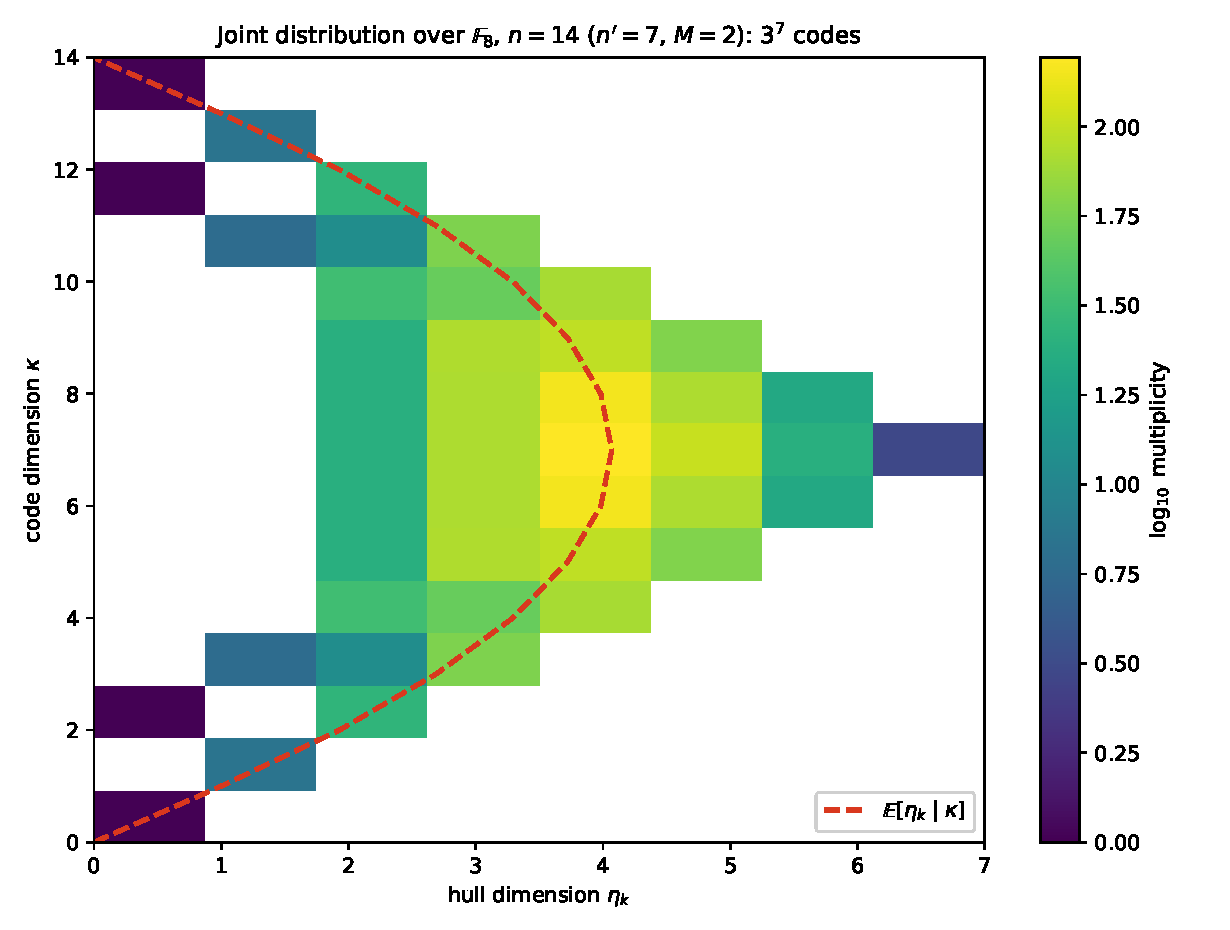
\includegraphics[width=0.78\textwidth]{fig5_joint_F8_n14.pdf}
\caption{Exact joint code-dimension and $1$-Galois-hull multiplicity map for all
$3^7=2{,}187$ cyclic codes of repeated-root length $n=14$ ($n'=7$, $M=2$) over
$\F_8$, with the exact rational conditional expectation curve
$\mathbb E[\eta_1\mid\kappa]$ overlaid ( peaking at $533/131\approx 4.069$ at
$\kappa=7$).}
\label{fig:joint-F8}
\end{figure}

\begin{example}[Odd-characteristic constacyclic versus negacyclic codes over $\F_9$]\label{ex:F9-constacyclic}
Let $\A=\F_9=\F_3(i)$ with $i^2+1=0$ ($p=3$, $e=2$, $m_1=1$), $k=1$, and
$n=12=4\cdot 3^1$ ($n'=4$, $M=3$). Compare two distinct compatible units:
\begin{enumerate}
\item[\textup{(a)}] Take $\lambda_{1,0}=i$, so the length-$12$ constacyclic shift
is $\lambda_1=i^3=-i\neq\lambda_{1,0}$. Since $i^{1+3^{2-1}}=i^4=1$, compatibility
holds; $x^4-i=(x^2+x-i)(x^2-x-i)$ factors into a single $\tau_{1,1}$-pair of
degree $2$, giving one orbit $(a_1,w_1)=(2,2)$, $4^2=16$ codes across $7$ cells,
$2$ LCD codes, $10$ SO/DC codes, $4$ self-dual codes, $\mathbb E[\eta_1]=2\cdot 2
\cdot(7/8)=7/2$, and $\Var(\eta_1)=2^2\cdot(15/16)=15/4$.
\item[\textup{(b)}] Take $\lambda_{1,0}=-1$, so $\lambda_1=(-1)^3=-1$ (negacyclic).
Now $x^4+1$ splits completely over $\F_9$ into four linear factors forming two
$\tau_{1,1}$-pairs $(2,1),(2,1)$: there are $4^4=256$ codes across $22$ cells,
$4$ LCD codes, $100$ SO/DC codes, and $4^2=16$ self-dual codes. Notice that
$\mathbb E[\eta_1]=2\cdot(7/4)=7/2$ coincides with \textup{(a)}, whereas
$\Var(\eta_1)=2\cdot(15/16)=15/8$ is halved because $w_O^2$ drops from $4$ to
$1+1=2$. By contrast, at cyclic shift $\lambda_{1,0}=\lambda_1=1$ over $\F_9$
($n=24=8\cdot 3$, Table~\ref{tab:summary-families}), four self-reciprocal orbits
appear and $M=3$ is odd, forcing $N_{\mathrm{SD}}=0$ by \eqref{eq:SD-count}.
\end{enumerate}
\end{example}

\begin{example}[Non-split affine algebra $\F_4\times\F_{16}$ over $\F_4$]\label{ex:mixed-F4-F16}
Consider $\A=\F_4[X]/\langle X(X^2+X+\omega)\rangle\cong K_1\times K_2$ over
$\F_4=\F_2(\omega)$, where $K_1=\F_4$ ($m_1=1$, $d_1=2$) and $K_2=\F_{16}$
($m_2=2$, $d_2=4$); since $m_2=2>1$, $\A$ lies strictly outside split-algebra
frameworks such as \cite{debnathAffine2026}. Take $n=10=5\cdot 2^1$ ($n'=5$,
$M=2$) and $k=1$, so ambient $\F_4$-dimension is $W=10(1+2)=30$.
\begin{enumerate}
\item[\textup{(a)}] At $\lambda_0=(1,1)$, $\lambda=\lambda_0^2=(1,1)$, $x^5-1$ has
$\tau_{1,1}$-orbits $(1,1),(2,2)$ over $\F_4$ and splits completely over $\F_{16}$
into one fixed point $(x+1)$ and one $4$-cycle under $\alpha\mapsto\alpha^{-8}=\alpha^7
\equiv\alpha^2\pmod 5$, contributing $\F_4$-weighted orbits $(1,2)$ and $(4,2)$.
Theorem~\ref{thm:main}\textup{(b)} enumerates all $3^8=6{,}561$ codes across $123$
joint $(\kappa,\eta_1)$ pairs, with $N_{\mathrm{LCD}}=2^4=16$,
$N_{\mathrm{SO}}=N_{\mathrm{DC}}=2\cdot 6\cdot 2\cdot 26=624$,
$N_{\mathrm{SD}}=1\cdot 3\cdot 1\cdot 3=9$, $\mathbb E[\eta_1]=23/3$, and
$\Var(\eta_1)=458/81$.
\item[\textup{(b)}] At the mixed unit $\lambda_0=(\omega,\beta)$,
$\lambda=(\omega^2,\beta^2)$ ($\beta^4+\beta+1=0$ in $\F_{16}$), component $K_1$
remains compatible ($\omega^3=1$), whereas component $K_2$ has
$\beta^{1+2^{4-1}}=\beta^9\neq 1$ and $x^5-\beta$ irreducible of degree $5$ over
$\F_{16}$ ($m_2\deg f=10$). By Theorem~\ref{thm:main}\textup{(a)},
$\Epoly^{(2)}(U,Z)=\Epoly_{K_1}^{(2)}(U,Z)\cdot(1+U^{10}+U^{20})$ over all
$27\cdot 3=81$ codes, giving $4\cdot 3=12$ LCD codes, $12$ SO codes, $12$ DC
codes, and $0$ self-dual codes.
\end{enumerate}
\end{example}

\begin{example}[Large-scale repeated-root families over $\F_{32}$]\label{ex:F32-large}
Let $\A=\F_{32}$ ($p=2$, $e=5$, $m_1=1$), $k=1$, $\lambda_{1,0}=\lambda_1=1$, and
consider the $2$-adic length tower $n_t=31\cdot 2^t$ ($n'=31$, $M=2^t$). Over
$\F_{32}$, $x^{31}-1$ splits into $N_F=31$ linear factors partitioned into
$(1,1)$ and three orbits of type $(10,1)$ ($|\mathcal O_1|=4$).
\begin{itemize}
\item At $t=1$ ($M=2$, $n=62$), Proposition~\ref{prop:algorithm} evaluates all
$3^{31}=617{,}673{,}396{,}283{,}947$ codes across $916$ $(\kappa,\eta_1)$ cells in
under $0.05\,\mathrm{s}$ (Figure~\ref{fig:joint-F32}), yielding $N_{\mathrm{LCD}}=16$,
$N_{\mathrm{SO}}=N_{\mathrm{DC}}=2\cdot 3{,}281^3=70{,}639{,}674{,}082$,
$N_{\mathrm{SD}}=1\cdot 3^3=27$, $\mathbb E[\eta_1]=1/3+30(5/9)=17$,
$\Var(\eta_1)=2/9+30(4/27)=14/3$, and mid-rate peak conditional expectation
\[
\mathbb E[\eta_1\mid\kappa=31]
 =\frac{937{,}013{,}336{,}624{,}311}{53{,}876{,}592{,}856{,}681}
 \approx 17.3918.
\]
\item At $t=2$ ($M=4$, $n=124$), the code space grows to
$5^{31}=4{,}656{,}612{,}873{,}077{,}392{,}578{,}125$ codes across $3{,}531$ cells
(evaluated in under $0.3\,\mathrm{s}$), with exact $N_{\mathrm{LCD}}=16$ unchanged
(probability $\approx 3.44\times 10^{-21}$),
$N_{\mathrm{SO}}=N_{\mathrm{DC}}=3\cdot 286{,}555^3=70{,}590{,}332{,}389{,}211{,}625$,
$N_{\mathrm{SD}}=1\cdot 5^3=125$, $\mathbb E[\eta_1]=184/5=36.8$, and
$\Var(\eta_1)=326/25=13.04$.
\end{itemize}
\end{example}

\begin{figure}[htbp]
\centering
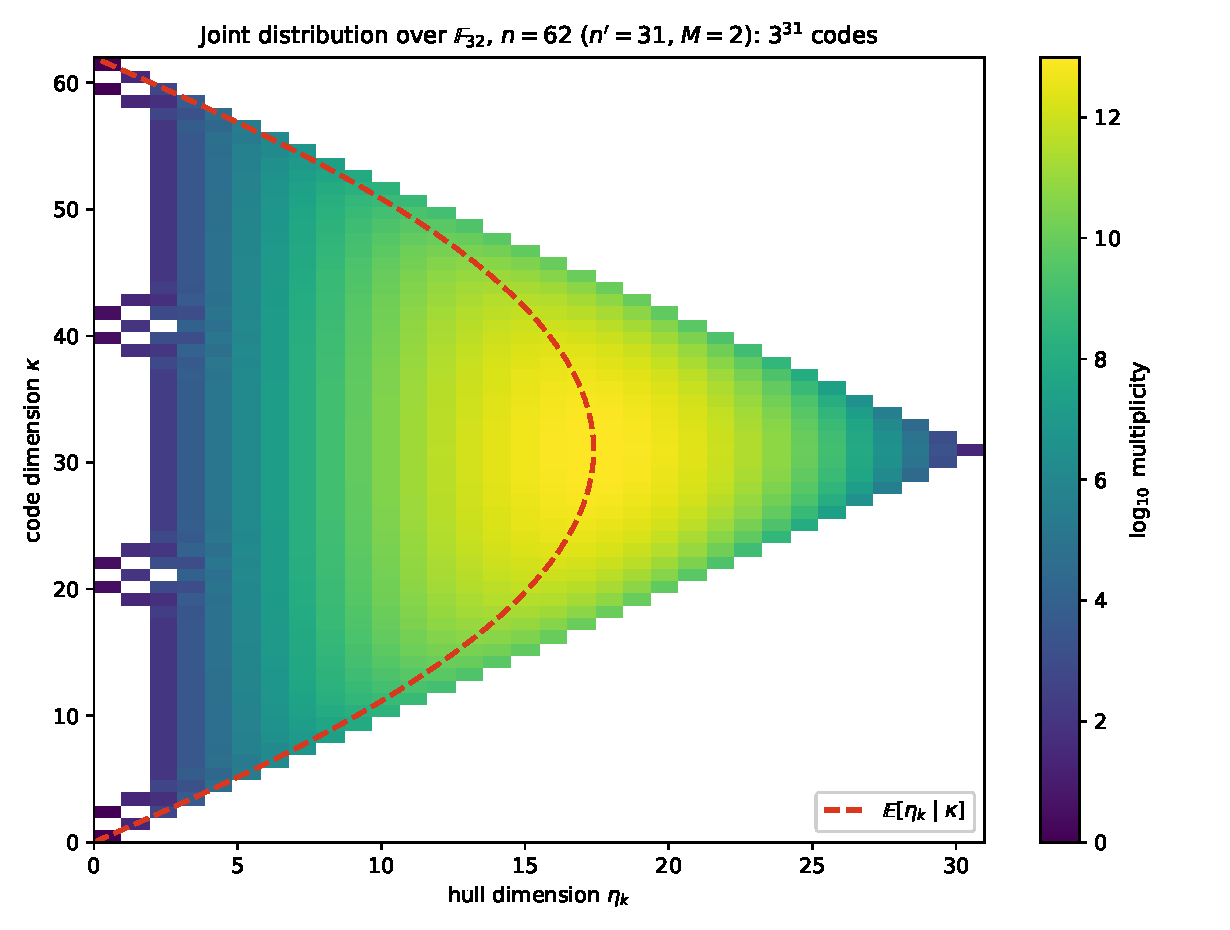
\includegraphics[width=0.78\textwidth]{fig6_joint_F32_n62.pdf}
\caption{Exact joint log-multiplicity distribution across all
$3^{31}=617{,}673{,}396{,}283{,}947$ cyclic codes of repeated-root length $n=62$
($n'=31$, $M=2$) over $\F_{32}$, with exact conditional expectation curve
$\mathbb E[\eta_1\mid\kappa]$ overlaid.}
\label{fig:joint-F32}
\end{figure}

\section{Conclusions}\label{sec:conclusions}

We have completely resolved the joint enumeration of code dimension $\kappa(C)$
and $k$-Galois hull dimension $\eta_k(C)$ across all $(M+1)^{N_F}$ labeled
$\A$-linear $\lambda$-constacyclic codes of arbitrary length $n=n'p^t$ ($M=p^t$,
$\gcd(n',p)=1$) over any finite commutative square-free affine algebra
$\A\cong\prod_{s=1}^{N}\F_{q^{m_s}}$ ($m_s\ge 1$) and any unit $\lambda\in\A^*$.
Passing to the unique $p^t$-th roots $\lambda_{s,0}\in K_s^*$ preserves twist
compatibility unchanged ($\lambda_{s,0}^{\,1+p^{d_s-k}}=1$), collapses all
incompatible components to trivial hulls, and turns $\dim_{K_s}\Hull_k(C_s(e))$ on
compatible components into a sum of cyclic edge minima $\min\{e_{O,i},M-e_{O,i+1}\}$
governed by universal $(M+1)\times(M+1)$ transfer matrices $T_{w_O}^{(M)}(U,Z)$.
This exact algebraic machinery answers the open counting problem posed by
Debnath et al.~\cite[p.~23]{debnathAffine2026} without split-algebra or
order-coprimality restrictions, contains the simple-root theory ($M=1$) as an
immediate special case, proves $p$-power invariance $2^{\sum_s|\Os|}$ of compatible $k$-Galois
LCD code counts, establishes unconditionally the exact single-orbit support
trapezoid and global Minkowski hull spectrum, yields closed rational mean,
variance, and conditional-moment laws alongside exact self-orthogonal,
dual-containing, and self-dual code counts, and runs in polynomial time even on
code spaces exceeding $10^{21}$.

Three natural open directions emerge directly from these results:
\begin{enumerate}
\item \emph{Simultaneous ring ramification and repeated-root lengths.} When $\A$
itself has nilpotent radical (for instance chain rings $\F_{p^m}[u]/\langle u^r\rangle$
or general finite commutative local rings~\cite{nortonSalagean2000,dinhLopezPermouth2004,jitmanZ4,talbi2022,pathakZ4,zhang2026})
and $p\mid n$ simultaneously, ambient rings cease to be principal ideal rings and
exponents are replaced by torsion filtrations; extending transfer-matrix
enumeration to that regime remains open.
\item \emph{Multi-twisted and quasi-twisted generalisations.} Extending our
$(M+1)$-state transfer operators from single-modulus constacyclic codes to
double cyclic, quasi-constacyclic, and multi-twisted code families~\cite{gao2023,eldinSole2026,eldinLeroy2026,aliabadi2026},
where $\A[x]/\langle x^n-\lambda\rangle$-ideals become rank-$r$ submodules of
$\bigoplus_{j=1}^{r}\A[x]/\langle x^{n_j}-\lambda_j\rangle$, involves non-abelian
Grassmannian / Hermite-normal-form local factors rather than scalar chains.
\item \emph{Minimum-distance stratification inside fixed $(\kappa,\eta_k)$ cells.}
Combining exact $(\kappa,\eta_k)$ cell multiplicities with torsion minimum-distance
bounds~\cite{castagnoli1991,nortonSalagean2000} to construct optimal repeated-root
EAQECCs with prescribed ebit count $c=\kappa-\eta_k$~\cite{brun2006,wildeBrun2008,guendaJitmanGulliver2018}
is an appealing direction for quantum code design.
\end{enumerate}

\section*{Declaration of competing interest}
The authors declare that they have no known competing financial interests or
personal relationships that could have appeared to influence the work reported in
this paper.

\section*{Data and code availability}
All exact coefficient tables, figures, and self-contained standard-library Python
verification scripts reproducing every calculation in this paper are provided in
the accompanying supplementary material package.

\section*{Funding}
This research did not receive any specific grant from funding agencies in the
public, commercial, or not-for-profit sectors.

\section*{Acknowledgements}
The authors thank the anonymous referees for their careful reading and constructive
suggestions.

\bibliographystyle{elsarticle-num}
\bibliography{references}
\end{document}
